% Options for packages loaded elsewhere
% Options for packages loaded elsewhere
\PassOptionsToPackage{unicode}{hyperref}
\PassOptionsToPackage{hyphens}{url}
%
\documentclass[
  ignorenonframetext,
]{beamer}
\newif\ifbibliography
\usepackage{pgfpages}
\setbeamertemplate{caption}[numbered]
\setbeamertemplate{caption label separator}{: }
\setbeamercolor{caption name}{fg=normal text.fg}
\beamertemplatenavigationsymbolsempty
% remove section numbering
\setbeamertemplate{part page}{
  \centering
  \begin{beamercolorbox}[sep=16pt,center]{part title}
    \usebeamerfont{part title}\insertpart\par
  \end{beamercolorbox}
}
\setbeamertemplate{section page}{
  \centering
  \begin{beamercolorbox}[sep=12pt,center]{section title}
    \usebeamerfont{section title}\insertsection\par
  \end{beamercolorbox}
}
\setbeamertemplate{subsection page}{
  \centering
  \begin{beamercolorbox}[sep=8pt,center]{subsection title}
    \usebeamerfont{subsection title}\insertsubsection\par
  \end{beamercolorbox}
}
% Prevent slide breaks in the middle of a paragraph
\widowpenalties 1 10000
\raggedbottom
\AtBeginPart{
  \frame{\partpage}
}
\AtBeginSection{
  \ifbibliography
  \else
    \frame{\sectionpage}
  \fi
}
\AtBeginSubsection{
  \frame{\subsectionpage}
}
\usepackage{iftex}
\ifPDFTeX
  \usepackage[T1]{fontenc}
  \usepackage[utf8]{inputenc}
  \usepackage{textcomp} % provide euro and other symbols
\else % if luatex or xetex
  \usepackage{unicode-math} % this also loads fontspec
  \defaultfontfeatures{Scale=MatchLowercase}
  \defaultfontfeatures[\rmfamily]{Ligatures=TeX,Scale=1}
\fi
\usepackage{lmodern}

\usetheme[]{Madrid}
\usefonttheme[]{structurebold}
\ifPDFTeX\else
  % xetex/luatex font selection
\fi
% Use upquote if available, for straight quotes in verbatim environments
\IfFileExists{upquote.sty}{\usepackage{upquote}}{}
\IfFileExists{microtype.sty}{% use microtype if available
  \usepackage[]{microtype}
  \UseMicrotypeSet[protrusion]{basicmath} % disable protrusion for tt fonts
}{}
\makeatletter
\@ifundefined{KOMAClassName}{% if non-KOMA class
  \IfFileExists{parskip.sty}{%
    \usepackage{parskip}
  }{% else
    \setlength{\parindent}{0pt}
    \setlength{\parskip}{6pt plus 2pt minus 1pt}}
}{% if KOMA class
  \KOMAoptions{parskip=half}}
\makeatother


\usepackage{longtable,booktabs,array}
\newcounter{none} % for unnumbered tables
\usepackage{calc} % for calculating minipage widths
\usepackage{caption}
% Make caption package work with longtable
\makeatletter
\def\fnum@table{\tablename~\thetable}
\makeatother
\usepackage{graphicx}
\makeatletter
\newsavebox\pandoc@box
\newcommand*\pandocbounded[1]{% scales image to fit in text height/width
  \sbox\pandoc@box{#1}%
  \Gscale@div\@tempa{\textheight}{\dimexpr\ht\pandoc@box+\dp\pandoc@box\relax}%
  \Gscale@div\@tempb{\linewidth}{\wd\pandoc@box}%
  \ifdim\@tempb\p@<\@tempa\p@\let\@tempa\@tempb\fi% select the smaller of both
  \ifdim\@tempa\p@<\p@\scalebox{\@tempa}{\usebox\pandoc@box}%
  \else\usebox{\pandoc@box}%
  \fi%
}
% Set default figure placement to htbp
\def\fps@figure{htbp}
\makeatother





\setlength{\emergencystretch}{3em} % prevent overfull lines

\providecommand{\tightlist}{%
  \setlength{\itemsep}{0pt}\setlength{\parskip}{0pt}}



 


\makeatletter
\@ifpackageloaded{tcolorbox}{}{\usepackage[skins,breakable]{tcolorbox}}
\@ifpackageloaded{fontawesome5}{}{\usepackage{fontawesome5}}
\definecolor{quarto-callout-color}{HTML}{909090}
\definecolor{quarto-callout-note-color}{HTML}{0758E5}
\definecolor{quarto-callout-important-color}{HTML}{CC1914}
\definecolor{quarto-callout-warning-color}{HTML}{EB9113}
\definecolor{quarto-callout-tip-color}{HTML}{00A047}
\definecolor{quarto-callout-caution-color}{HTML}{FC5300}
\definecolor{quarto-callout-color-frame}{HTML}{acacac}
\definecolor{quarto-callout-note-color-frame}{HTML}{4582ec}
\definecolor{quarto-callout-important-color-frame}{HTML}{d9534f}
\definecolor{quarto-callout-warning-color-frame}{HTML}{f0ad4e}
\definecolor{quarto-callout-tip-color-frame}{HTML}{02b875}
\definecolor{quarto-callout-caution-color-frame}{HTML}{fd7e14}
\makeatother
\makeatletter
\@ifpackageloaded{caption}{}{\usepackage{caption}}
\AtBeginDocument{%
\ifdefined\contentsname
  \renewcommand*\contentsname{Table of contents}
\else
  \newcommand\contentsname{Table of contents}
\fi
\ifdefined\listfigurename
  \renewcommand*\listfigurename{List of Figures}
\else
  \newcommand\listfigurename{List of Figures}
\fi
\ifdefined\listtablename
  \renewcommand*\listtablename{List of Tables}
\else
  \newcommand\listtablename{List of Tables}
\fi
\ifdefined\figurename
  \renewcommand*\figurename{Figure}
\else
  \newcommand\figurename{Figure}
\fi
\ifdefined\tablename
  \renewcommand*\tablename{Table}
\else
  \newcommand\tablename{Table}
\fi
}
\@ifpackageloaded{float}{}{\usepackage{float}}
\floatstyle{ruled}
\@ifundefined{c@chapter}{\newfloat{codelisting}{h}{lop}}{\newfloat{codelisting}{h}{lop}[chapter]}
\floatname{codelisting}{Listing}
\newcommand*\listoflistings{\listof{codelisting}{List of Listings}}
\makeatother
\makeatletter
\makeatother
\makeatletter
\@ifpackageloaded{caption}{}{\usepackage{caption}}
\@ifpackageloaded{subcaption}{}{\usepackage{subcaption}}
\makeatother

\usepackage{bookmark}
\IfFileExists{xurl.sty}{\usepackage{xurl}}{} % add URL line breaks if available
\urlstyle{same}
\hypersetup{
  pdftitle={第三章 周期信号的傅里叶级数表示},
  pdfauthor={马越},
  hidelinks,
  pdfcreator={LaTeX via pandoc}}


\title{\texorpdfstring{第三章
周期信号的傅里叶级数表示}{第三章 周期信号的傅里叶级数表示}}
\author{马越}
\date{}
\institute{北京理工大学机械与车辆学院 Email: yuema@bit.edu.cn}

\begin{document}
\frame{\titlepage}


\section{0.
傅里叶分析的历史回顾}\label{ux5085ux91ccux53f6ux5206ux6790ux7684ux5386ux53f2ux56deux987e}

\begin{frame}{引子}
\protect\phantomsection\label{ux5f15ux5b50}
\pandocbounded{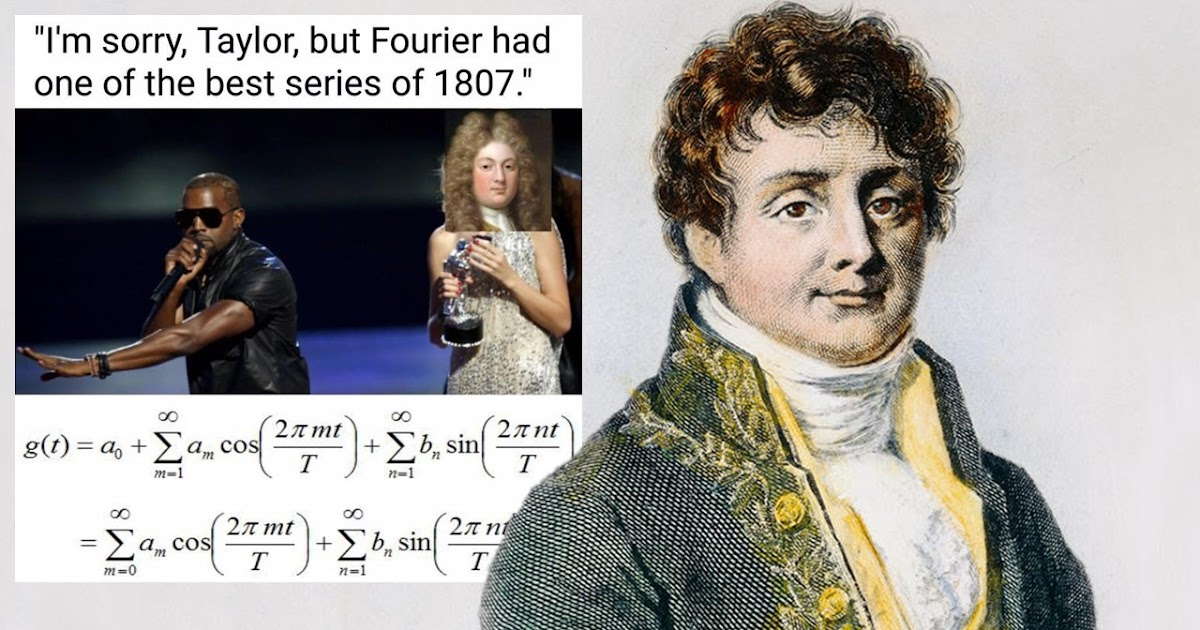
\includegraphics[keepaspectratio]{imglink/taylor_swift_fourier_series_maths_physics.png}}
\end{frame}

\begin{frame}{波动方程的诞生 (1747)}
\protect\phantomsection\label{ux6ce2ux52a8ux65b9ux7a0bux7684ux8bdeux751f-1747}
\textbf{达朗贝尔 (Jean le Rond d'Alembert)}

开启了将物理现象``数学化''的先河。他通过研究琴弦的受力，导出了历史上第一个偏微分方程。

\begin{block}{一维波动方程}
\protect\phantomsection\label{ux4e00ux7ef4ux6ce2ux52a8ux65b9ux7a0b}
\[ \frac{\partial^2 u}{\partial t^2} = v^2 \frac{\partial^2 u}{\partial x^2} \]

\begin{itemize}
\tightlist
\item
  \textbf{\(u(x, t)\)}：弦在 \(t\) 时刻、位置 \(x\) 处的位移。
\item
  \textbf{\(v\)}：波在弦上的传播速度。
\end{itemize}
\end{block}

\begin{block}{达朗贝尔解}
\protect\phantomsection\label{ux8fbeux6717ux8d1dux5c14ux89e3}
他指出，波动方程的通解可以表示为两个行进波的叠加：
\[ u(x, t) = f(x - vt) + g(x + vt) \]
\end{block}
\end{frame}

\begin{frame}{叠加原理的物理直觉 (1753)}
\protect\phantomsection\label{ux53e0ux52a0ux539fux7406ux7684ux7269ux7406ux76f4ux89c9-1753}
\textbf{丹尼尔·伯努利 (Daniel Bernoulli)}

是一位极具物理洞察力的科学家。他通过观察乐器的泛音现象，提出了划时代的观点：\textbf{复杂的振动是由简单频率的简谐振动叠加而成的。}

\begin{block}{伯努利解（三角级数雏形）}
\protect\phantomsection\label{ux4f2fux52aaux5229ux89e3ux4e09ux89d2ux7ea7ux6570ux96cfux5f62}
对于两端固定的琴弦（长度为 \(L\)），他给出了级数形式的解：
\[ u(x, t) = \sum_{n=1}^{\infty} A_n \sin\left(\frac{n\pi x}{L}\right) \cos\left(\frac{n\pi vt}{L}\right) \]

\begin{itemize}
\tightlist
\item
  \textbf{物理意义}：每一个 \(n\) 对应一个``模态''。\(n=1\)
  是基音，\(n > 1\) 是泛音。
\item
  \textbf{争议点}：当时的数学界无法接受``无穷多个连续函数相加可以组合成任意形状''这一观点。
\end{itemize}
\end{block}
\end{frame}

\begin{frame}{正交性与系数推导 (1777)}
\protect\phantomsection\label{ux6b63ux4ea4ux6027ux4e0eux7cfbux6570ux63a8ux5bfc-1777}
\textbf{欧拉 (Leonhard Euler)}
展现了他惊人的数学推导能力。虽然他对伯努利结论的普适性持怀疑态度，但他却亲手推导出了计算这些系数的关键数学工具。

\begin{block}{三角函数的正交性}
\protect\phantomsection\label{ux4e09ux89d2ux51fdux6570ux7684ux6b63ux4ea4ux6027}
欧拉发现，在特定区间内，不同频率的正弦函数乘积的积分为零：
\[ \int_0^L \sin\left(\frac{m\pi x}{L}\right) \sin\left(\frac{n\pi x}{L}\right) dx = \begin{cases} L/2, & m = n \\ 0, & m \neq n \end{cases} \]
\end{block}

\begin{block}{系数确定公式}
\protect\phantomsection\label{ux7cfbux6570ux786eux5b9aux516cux5f0f}
基于正交性，欧拉给出了如何从初始波形 \(f(x)\) 中提取系数 \(A_n\)
的公式（这正是后来傅里叶系数的标准形式）：
\[ A_n = \frac{2}{L} \int_0^L f(x) \sin\left(\frac{n\pi x}{L}\right) dx \]
\end{block}
\end{frame}

\begin{frame}{傅里叶级数}
\protect\phantomsection\label{ux5085ux91ccux53f6ux7ea7ux6570}
\textbf{傅里叶（Joseph
Fourier）}在格勒诺布尔的火炉旁研究\textbf{热传导}时，受到了实际物理过程的强烈启发，这直接促成了\textbf{傅里叶级数}和\textbf{热传导方程}的诞生。

场景：一根细长金属棒，两端保持固定低温（例如0°C），初始时棒子中间被局部加热，形成非均匀温度分布-光滑的近似的驼峰形状

\begin{columns}[T]
\begin{column}{0.5\linewidth}
\pandocbounded{\includegraphics[keepaspectratio]{imglink/en-thermodynamics-heat-equation-diffusion-equation.mp4}}
\end{column}

\begin{column}{0.5\linewidth}
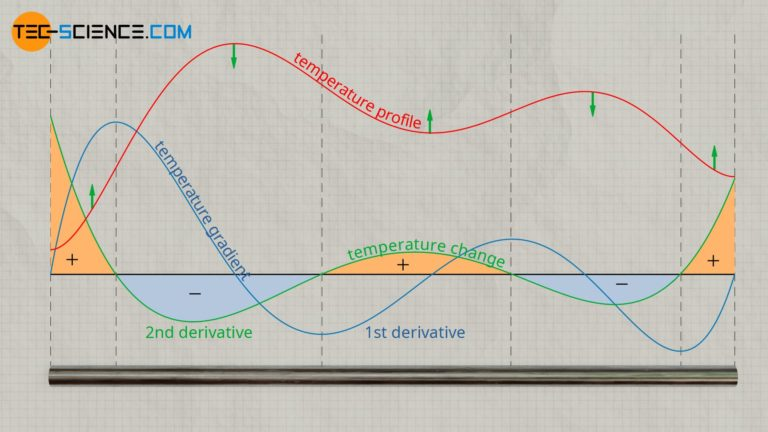
\includegraphics[width=1\linewidth,height=\textheight,keepaspectratio]{imglink/en-thermodynamics-heat-equation-diffusion-equation-temperature-gradient-768x432.png}
\end{column}
\end{columns}

热量流动方向总是从高温到低温（由曲率决定）：

凹向下（曲率正）→ 热量净流入，温度上升；凹向上（曲率负）→
热量净流出，温度下降。

\[\frac{\partial T}{\partial t} = \alpha \frac{\partial^2 T}{\partial x^2}\]
\end{frame}

\begin{frame}{傅里叶级数}
\protect\phantomsection\label{ux5085ux91ccux53f6ux7ea7ux6570-1}
为了求解这个偏微分方程，傅里叶引入了分离变量法，得到用正弦函数（或余弦）展开初始温度分布的想法------这就是傅里叶级数的诞生。

\begin{columns}[T]
\begin{column}{0.5\linewidth}
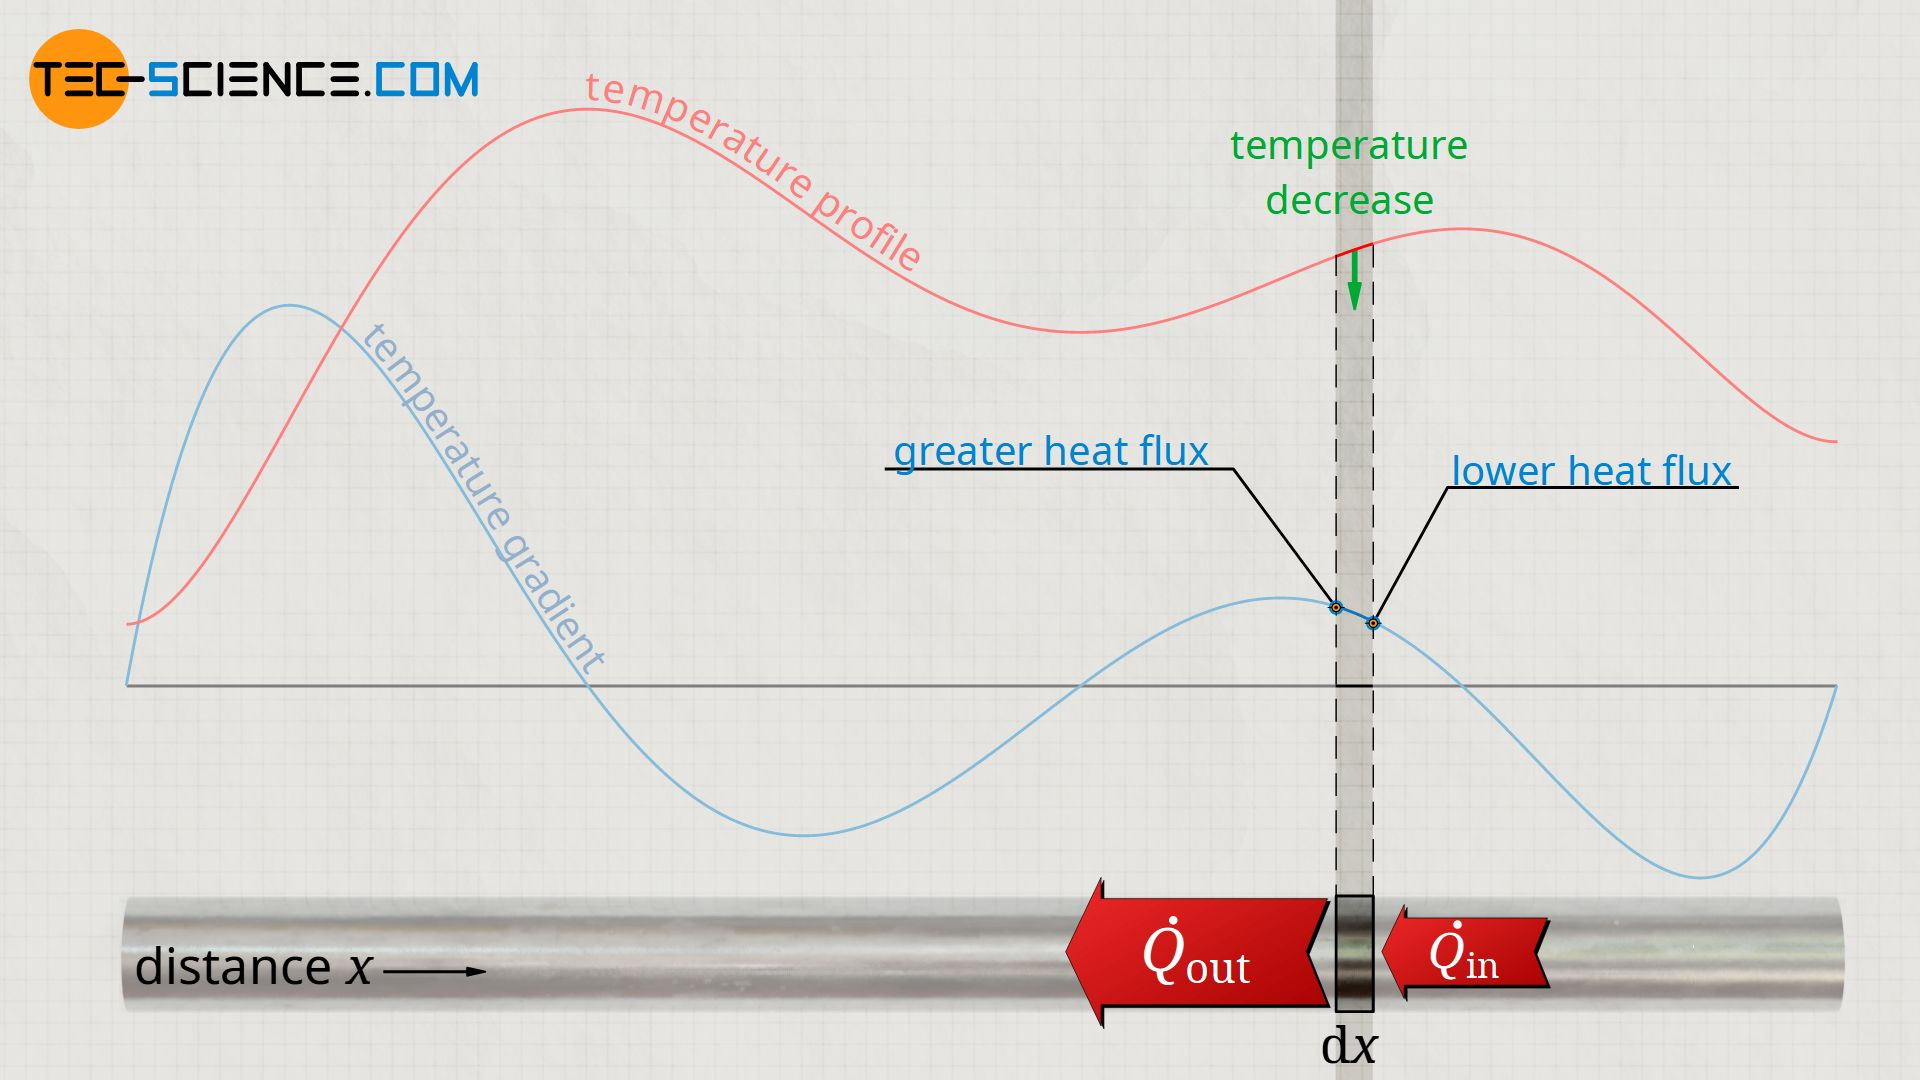
\includegraphics[width=0.6\linewidth,height=\textheight,keepaspectratio]{imglink/en-thermodynamics-heat-equation-diffusion-equation-temperature-decrease.png}
\end{column}

\begin{column}{0.5\linewidth}
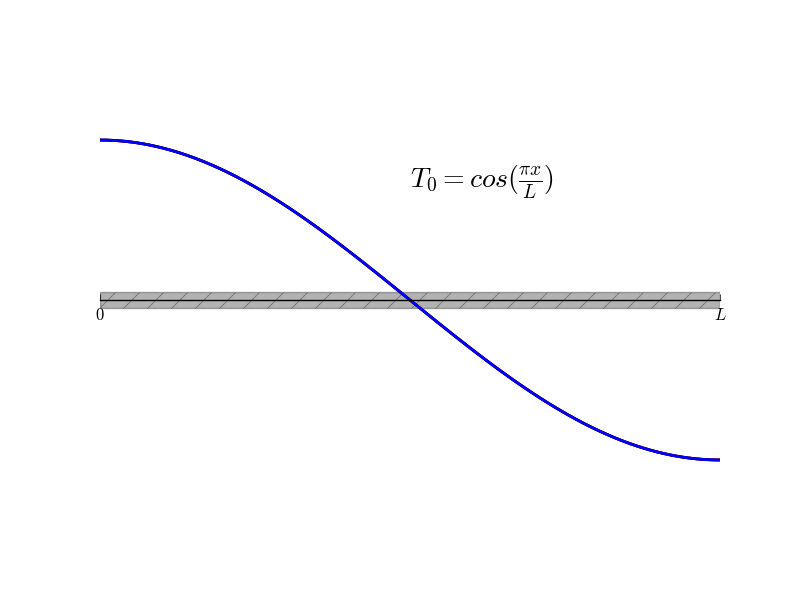
\includegraphics[width=0.6\linewidth,height=\textheight,keepaspectratio]{imglink/v2-29585c43f35579534d35d919df68d8d7_1440w.png}
\end{column}
\end{columns}

1807 年 12 月 21 日，傅里叶向法兰西学会提交了论文 《固体中的热传导》
(Sur la propagation de la chaleur dans les corps solides)。

\[ f(x) = \frac{a_0}{2} + \sum_{n=1}^{\infty} [a_n \cos(nx) + b_n \sin(nx)] \]

傅里叶的数学洞察本质是：\textbf{物理上热量会``抹平''尖锐的温度差异，而数学上可以用无穷多个光滑的正弦波无限逼近任何（合理）的初始分布}。高频（短波长）分量衰减最快
→ 温度曲线逐渐变光滑。

这两种看似无关的现象在 1822
年的《热的解析理论》中被统一起来，成为分析数学与物理的桥梁。
\end{frame}

\begin{frame}{拉格朗日的执念与傅里叶的胜利}
\protect\phantomsection\label{ux62c9ux683cux6717ux65e5ux7684ux6267ux5ff5ux4e0eux5085ux91ccux53f6ux7684ux80dcux5229}
审查委员会里: 拉普拉斯、拉格朗日、蒙日。

拉格朗日站起来强烈抗议：他在年轻时研究弦振动就否定过这种级数，他绝不相信无穷个三角级数能表示不连续函数。

\begin{tcolorbox}[enhanced jigsaw, arc=.35mm, bottomrule=.15mm, bottomtitle=1mm, breakable, colback=white, colbacktitle=quarto-callout-note-color!10!white, colframe=quarto-callout-note-color-frame, coltitle=black, left=2mm, leftrule=.75mm, opacityback=0, opacitybacktitle=0.6, rightrule=.15mm, title=\textcolor{quarto-callout-note-color}{\faInfo}\hspace{0.5em}{Note}, titlerule=0mm, toprule=.15mm, toptitle=1mm]

结果：论文被搁置了 15
年，直到拉格朗日去世后，傅里叶才正式出版了他的著作。

\end{tcolorbox}

数学史评价：傅里叶不是在象牙塔里推导公式，他是在格勒诺布尔的火炉旁，看着热量如何抹平温度的褶皱，感悟到了宇宙的语言------频率。

``对自然界的深刻研究是数学发现最丰饶的源泉。'' ------ 约瑟夫·傅里叶

\begin{block}{完善：从直觉跨入严密分析}
\protect\phantomsection\label{ux5b8cux5584ux4eceux76f4ux89c9ux8de8ux5165ux4e25ux5bc6ux5206ux6790}
\begin{itemize}
\tightlist
\item
  {狄利克雷
  (1829)}：给出了著名的``狄利克雷条件''。这是数学史上第一次明确了三角级数表示法的适用边界。
\item
  {从级数到变换}：通过将周期趋于无穷大，实现了从周期信号（加权和）到非周期信号（积分）的飞跃。
\item
  {认知结论}：傅里叶分析不仅是计算工具，更是一种将``时域''映射到``频域''的哲学观。
\end{itemize}
\end{block}
\end{frame}

\begin{frame}{离散化：高斯的秘密遗稿}
\protect\phantomsection\label{ux79bbux6563ux5316ux9ad8ux65afux7684ux79d8ux5bc6ux9057ux7a3f}
虽然教材通常从1965年讲起，但史料显示：

\begin{columns}[T]
\begin{column}{0.5\linewidth}
\begin{block}{{1805年 高斯 (Gauss)}}
\protect\phantomsection\label{ux5e74-ux9ad8ux65af-gauss}
为计算小行星轨道，已发明类似FFT的技巧。但他认为这只是``小把戏''，未曾发表
。
\end{block}
\end{column}

\begin{column}{0.5\linewidth}
\begin{block}{{18-19世纪 天体观测}}
\protect\phantomsection\label{ux4e16ux7eaa-ux5929ux4f53ux89c2ux6d4b}
天文学数据天生是离散的，这为数值分析和傅里叶方法的结合提供了第二舞台。
\end{block}
\end{column}
\end{columns}

\begin{block}{1965：FFT 与数字文明的开启}
\protect\phantomsection\label{fft-ux4e0eux6570ux5b57ux6587ux660eux7684ux5f00ux542f}
\begin{itemize}
\tightlist
\item
  {Cooley-Tukey 算法}：冷战期间为监测核试验而``再发现''FFT。
\item
  {计算量级跳变}：将 \(O(N^2)\) 降至 \(O(N \log N)\)。
\item
  {应用爆发}：雷达、通信（4G/5G）、图像处理（JPEG）、语音识别。
\end{itemize}

如果没有FFT，现代智能手机的信号处理将需要几百倍的功耗。
\end{block}
\end{frame}

\begin{frame}{目录}
\protect\phantomsection\label{toc0}
\begin{itemize}
\tightlist
\item
  \hyperlink{sec31}{\textbf{1. 线性时不变系统对复指数信号的响应}}
\item
  \hyperlink{sec32}{2. 连续时间周期信号的傅里叶级数表示}
\item
  \hyperlink{sec33}{3. 连续时间傅里叶级数的收敛}
\item
  \hyperlink{sec34}{4. 连续时间傅里叶级数的性质}
\item
  \hyperlink{35}{5. 离散时间周期信号的傅里叶级数表示}
\item
  \hyperlink{sec36}{6. 离散时间傅里叶级数的性质}
\item
  \hyperlink{sec37}{7. 傅里叶级数与线性时不变系统}
\item
  \hyperlink{sec38}{8. 滤波}

  \begin{itemize}
  \tightlist
  \item
    \hyperlink{sec381}{频率成形滤波器}
  \item
    \hyperlink{sec382}{频率选择性滤波器}
  \item
    \hyperlink{sec383}{用微分方程描述的连续时间滤波器}
  \item
    \hyperlink{sec383}{用差分方程描述的离散时间滤波器}
  \end{itemize}
\end{itemize}
\end{frame}

\section{1. 线性时不变系统对复指数信号的响应}\label{sec31}

\begin{frame}{回顾与联系}
\protect\phantomsection\label{ux56deux987eux4e0eux8054ux7cfb}
{\def\LTcaptype{none} % do not increment counter
\begin{longtable}[]{@{}
  >{\raggedright\arraybackslash}p{(\linewidth - 6\tabcolsep) * \real{0.2500}}
  >{\raggedright\arraybackslash}p{(\linewidth - 6\tabcolsep) * \real{0.2500}}
  >{\raggedright\arraybackslash}p{(\linewidth - 6\tabcolsep) * \real{0.2500}}
  >{\raggedright\arraybackslash}p{(\linewidth - 6\tabcolsep) * \real{0.2500}}@{}}
\toprule\noalign{}
\begin{minipage}[b]{\linewidth}\raggedright
\end{minipage} & \begin{minipage}[b]{\linewidth}\raggedright
\(\mathbb{R}^{n}\)
\end{minipage} & \begin{minipage}[b]{\linewidth}\raggedright
DT 信号 \(\mathbb{C}^{\mathbb{Z}}\)
\end{minipage} & \begin{minipage}[b]{\linewidth}\raggedright
CT 信号
\end{minipage} \\
\midrule\noalign{}
\endhead
\textbf{基 (basis)} &
\(\left\{\mathbf{e}_{1}, \ldots, \mathbf{e}_{n}\right\}\) &
\(\left\{\delta_{k}: k \in \mathbb{Z}\right\}\) &
\(\left\{\delta_{\tau}: \tau \in \mathbb{R}\right\}^{1}\) \\
\textbf{一般信号 \(x\)} & \(x=\sum_{k=1}^{n} x_{k} \mathbf{e}_{k}\) &
\(x=\sum_{k \in \mathbb{Z}} x[k] \delta_{k}\) &
\(x=\int_{\mathbb{R}} x(\tau) \delta_{\tau} d \tau\) \\
\textbf{线性变换下的像} & & & \\
\textbf{基的像} &
\(\left\{\mathbf{f}_{1}, \ldots, \mathbf{f}_{n}\right\}\) &
\(\left\{h_{k}: k \in \mathbb{Z}\right\}\) &
\(\left\{h_{\tau}: \tau \in \mathbb{R}\right\}\) \\
\textbf{一般信号 \(x\) 的像} &
\(A x=\sum_{k=1}^{n} x_{k} \mathbf{f}_{k}\) &
\(T(x)=\sum_{k \in \mathbb{Z}} x[k] h_{k}\) &
\(T(x)=\int_{\mathbb{R}} x(\tau) h_{\tau} d \tau\) \\
\textbf{LTI 系统} & - & \(T(x)=x * h\) & \(T(x)=x * h\) \\
\bottomrule\noalign{}
\end{longtable}
}

注：并非``基''的标准用法；需结合下一行的积分表示来理解。
\end{frame}

\begin{frame}{特征值与特征向量}
\protect\phantomsection\label{ux7279ux5f81ux503cux4e0eux7279ux5f81ux5411ux91cf}
在线性代数中，\(v \in \mathbb{R}^{n}\) 是矩阵 \(A\) 的特征向量
(eigenvector)，其对应的特征值 (eigenvalue) 为 \(\lambda\)，如果：

\[
A v=\lambda v
\]

假设 \(A\) 有 \(n\) 个不同的特征值
\(\lambda_{1}, \ldots, \lambda_{n}\)，分别对应特征向量
\(v_{1}, \ldots, v_{n}\)。

\begin{itemize}
\tightlist
\item
  \(v_{1}, \ldots, v_{n}\) 构成 \(\mathbb{R}^{n}\) 的一组基，即
  \(\forall x \in \mathbb{R}^{n}\) 都有以下表示：
\end{itemize}

\[
x=\sum_{k=1}^{n} a_{k} v_{k}
\]

\begin{itemize}
\tightlist
\item
  \(x\) 在 \(A\) 作用下的像：
\end{itemize}

\[
A x=\sum_{k=1}^{n} a_{k} A v_{k}=\sum_{k=1}^{n} a_{k} \lambda_{k} v_{k}
\]
\end{frame}

\begin{frame}{基变换 (Change of Basis)}
\protect\phantomsection\label{ux57faux53d8ux6362-change-of-basis}
{\def\LTcaptype{none} % do not increment counter
\begin{longtable}[]{@{}
  >{\centering\arraybackslash}p{(\linewidth - 4\tabcolsep) * \real{0.3333}}
  >{\centering\arraybackslash}p{(\linewidth - 4\tabcolsep) * \real{0.3333}}
  >{\centering\arraybackslash}p{(\linewidth - 4\tabcolsep) * \real{0.3333}}@{}}
\toprule\noalign{}
\begin{minipage}[b]{\linewidth}\centering
\end{minipage} & \begin{minipage}[b]{\linewidth}\centering
标准基
\end{minipage} & \begin{minipage}[b]{\linewidth}\centering
\(A\) 的''特征基''
\end{minipage} \\
\midrule\noalign{}
\endhead
\textbf{基向量} &
\(\left\{\mathbf{e}_{1}, \ldots, \mathbf{e}_{n}\right\}\) &
\(\left\{v_{1}, \ldots, v_{n}\right\}\) \\
\textbf{分解} & \(x=\sum_{k=1}^{n} x_{k} \mathbf{e}_{k}\) &
\(x=\sum_{k=1}^{n} a_{k} v_{k}\) \\
\textbf{\(A\) 作用下的像} & \(A x=\sum_{k=1}^{n} x_{k} \mathbf{f}_{k}\)
& \(A x=\sum_{k=1}^{n} a_{k} \lambda_{k} v_{k}\) \\
\bottomrule\noalign{}
\end{longtable}
}

\(x\) 和 \(A x\) 的展开：

\begin{itemize}
\tightlist
\item
  在标准基下：系数 \(\left\{x_{k}\right\}\) 相同，基向量不同
  \(\left\{\mathbf{e}_{k}\right\} \mapsto\left\{\mathbf{f}_{k}\right\}\)（卷积/叠加积分）
\item
  在特征基下：基向量 \(\left\{v_{k}\right\}\) 相同，系数不同
  \(\left\{a_{k}\right\} \mapsto\left\{\lambda_{k} a_{k}\right\}\)（乘法）
\end{itemize}
\end{frame}

\begin{frame}{基变换 (信号与系统)}
\protect\phantomsection\label{ux57faux53d8ux6362-ux4fe1ux53f7ux4e0eux7cfbux7edf}
{\def\LTcaptype{none} % do not increment counter
\begin{longtable}[]{@{}
  >{\raggedright\arraybackslash}p{(\linewidth - 6\tabcolsep) * \real{0.2500}}
  >{\raggedright\arraybackslash}p{(\linewidth - 6\tabcolsep) * \real{0.2500}}
  >{\raggedright\arraybackslash}p{(\linewidth - 6\tabcolsep) * \real{0.2500}}
  >{\raggedright\arraybackslash}p{(\linewidth - 6\tabcolsep) * \real{0.2500}}@{}}
\toprule\noalign{}
\begin{minipage}[b]{\linewidth}\raggedright
DT
\end{minipage} & \begin{minipage}[b]{\linewidth}\raggedright
\end{minipage} & \begin{minipage}[b]{\linewidth}\raggedright
标准基
\end{minipage} & \begin{minipage}[b]{\linewidth}\raggedright
``特征基''
\end{minipage} \\
\midrule\noalign{}
\endhead
& 基向量 & \(\left\{\delta_{k}: k \in \mathbb{Z}\right\}\) & ？ \\
& 分解 & \(x=\sum_{k \in \mathbb{Z}} x[k] \delta_{k}\) & ？ \\
& \(T\) 作用下的像 & \(T(x)=\sum_{k \in \mathbb{Z}} x[k] h_{k}\) & ？ \\
CT & & ``标准基'' & ``特征基'' \\
& 基向量 & \(\left\{\delta_{\tau}: \tau \in \mathbb{R}\right\}\) & ？ \\
& 分解 & \(x=\int_{\mathbb{R}} x(\tau) \delta_{\tau} d \tau\) & ？ \\
& \(T\) 作用下的像 & \(T(x)=\int_{\mathbb{R}} x(\tau) h_{\tau} d \tau\)
& ？ \\
\bottomrule\noalign{}
\end{longtable}
}
\end{frame}

\begin{frame}{LTI 系统的特征值与特征函数}
\protect\phantomsection\label{lti-ux7cfbux7edfux7684ux7279ux5f81ux503cux4e0eux7279ux5f81ux51fdux6570}
\textbf{CT 指数信号 \(e^{s t}\)}

\[
T\left(e^{s t}\right)=\int_{\mathbb{R}} h(\tau) e^{s(t-\tau)} d \tau=e^{s t} \int_{\mathbb{R}} h(\tau) e^{-s \tau} d \tau,
\]

{ \(e^{s t}\) 是 \(T\) 的\textbf{特征函数}，对应的\textbf{特征值} }为：

\[
H(s)=\int_{\mathbb{R}} h(\tau) e^{-s \tau} d \tau \quad \text { (系统函数) } 
\]

\textbf{DT 指数信号 \(z^{n}\)}

\[
T\left(z^{n}\right)=\sum_{k \in \mathbb{Z}} h[k] z^{n-k}=z^{n} \sum_{k \in \mathbb{Z}} h[k] z^{-k},
\]

{ \(z^{n}\) 是 \(T\) 的\textbf{特征函数}，对应的\textbf{特征值} }为：

\[
H(z)=\sum_{k \in \mathbb{Z}} h[k] z^{-k} \quad \text { (系统函数) }
\]
\end{frame}

\begin{frame}{对特征函数线性组合的响应}
\protect\phantomsection\label{ux5bf9ux7279ux5f81ux51fdux6570ux7ebfux6027ux7ec4ux5408ux7684ux54cdux5e94}
\textbf{CT (连续时间)}

\[
T\left(\sum_{k} a_{k} e^{s_{k} t}\right)=\sum_{k} a_{k} H\left(s_{k}\right) e^{s_{k} t}
\]

\textbf{DT (离散时间)}

\[
T\left(\sum_{k} a_{k} z_{k}^{n}\right)=\sum_{k} a_{k} H\left(z_{k}\right) z_{k}^{n}
\]

输入 vs.~输出

\begin{itemize}
\tightlist
\item
  相同的指数函数的线性组合
\item
  系数发生变化：\(\left\{a_{k}\right\} \mapsto\left\{H\left(s_{k}\right) a_{k}\right\} /\left\{H\left(z_{k}\right) a_{k}\right\}\)
\end{itemize}
\end{frame}

\begin{frame}{基变换 (信号与系统)}
\protect\phantomsection\label{ux57faux53d8ux6362-ux4fe1ux53f7ux4e0eux7cfbux7edf-1}
{\def\LTcaptype{none} % do not increment counter
\begin{longtable}[]{@{}
  >{\centering\arraybackslash}p{(\linewidth - 4\tabcolsep) * \real{0.3333}}
  >{\centering\arraybackslash}p{(\linewidth - 4\tabcolsep) * \real{0.3333}}
  >{\centering\arraybackslash}p{(\linewidth - 4\tabcolsep) * \real{0.3333}}@{}}
\toprule\noalign{}
\begin{minipage}[b]{\linewidth}\centering
\end{minipage} & \begin{minipage}[b]{\linewidth}\centering
标准基
\end{minipage} & \begin{minipage}[b]{\linewidth}\centering
\(A\) 的''特征基''
\end{minipage} \\
\midrule\noalign{}
\endhead
\textbf{基向量} &
\(\left\{\mathbf{e}_{1}, \ldots, \mathbf{e}_{n}\right\}\) &
\(\left\{v_{1}, \ldots, v_{n}\right\}\) \\
\textbf{分解} & \(x=\sum_{k=1}^{n} x_{k} \mathbf{e}_{k}\) &
\(x=\sum_{k=1}^{n} a_{k} v_{k}\) \\
\textbf{\(A\) 作用下的像} & \(A x=\sum_{k=1}^{n} x_{k} \mathbf{f}_{k}\)
& \(A x=\sum_{k=1}^{n} a_{k} \lambda_{k} v_{k}\) \\
\bottomrule\noalign{}
\end{longtable}
}

对照：

{\def\LTcaptype{none} % do not increment counter
\begin{longtable}[]{@{}
  >{\raggedright\arraybackslash}p{(\linewidth - 6\tabcolsep) * \real{0.2500}}
  >{\raggedright\arraybackslash}p{(\linewidth - 6\tabcolsep) * \real{0.2500}}
  >{\raggedright\arraybackslash}p{(\linewidth - 6\tabcolsep) * \real{0.2500}}
  >{\raggedright\arraybackslash}p{(\linewidth - 6\tabcolsep) * \real{0.2500}}@{}}
\toprule\noalign{}
\begin{minipage}[b]{\linewidth}\raggedright
DT
\end{minipage} & \begin{minipage}[b]{\linewidth}\raggedright
\end{minipage} & \begin{minipage}[b]{\linewidth}\raggedright
标准基
\end{minipage} & \begin{minipage}[b]{\linewidth}\raggedright
``特征基''
\end{minipage} \\
\midrule\noalign{}
\endhead
& 基向量 & \(\left\{\delta_{k}: k \in \mathbb{Z}\right\}\) & \(z^n\) \\
& 分解 & \(x=\sum_{k \in \mathbb{Z}} x[k] \delta_{k}\) & 傅里叶/Z
变换 \\
& \(T\) 作用下的像 & \(T(x)=\sum_{k \in \mathbb{Z}} x[k] h_{k}\) &
\(H(z) z^n\) \\
CT & & \textbf{``标准基''} & \textbf{``特征基''} \\
& 基向量 & \(\left\{\delta_{\tau}: \tau \in \mathbb{R}\right\}\) &
\(e^{st}\) \\
& 分解 & \(x=\int_{\mathbb{R}} x(\tau) \delta_{\tau} d \tau\) &
傅里叶/拉普拉斯变换 \\
& \(T\) 作用下的像 & \(T(x)=\int_{\mathbb{R}} x(\tau) h_{\tau} d \tau\)
& \(H(s) e^{st}\) \\
\bottomrule\noalign{}
\end{longtable}
}
\end{frame}

\begin{frame}{问题}
\protect\phantomsection\label{ux95eeux9898}
\begin{itemize}
\tightlist
\item
  哪些函数可以是指数函数的线性组合？
\item
  如何找到系数 \(a_{k}\)？
\end{itemize}

傅里叶分析重点关注 CT 中的 \(e^{j \omega t}\) 和 DT 中的
\(e^{j \omega n}\)。
\end{frame}

\begin{frame}{目录}
\protect\phantomsection\label{toc1}
\begin{itemize}
\tightlist
\item
  \hyperlink{sec31}{1. 线性时不变系统对复指数信号的响应}
\item
  \hyperlink{sec32}{\textbf{2. 连续时间周期信号的傅里叶级数表示}}
\item
  \hyperlink{sec33}{3. 连续时间傅里叶级数的收敛}
\item
  \hyperlink{sec34}{4. 连续时间傅里叶级数的性质}
\item
  \hyperlink{35}{5. 离散时间周期信号的傅里叶级数表示}
\item
  \hyperlink{sec36}{6. 离散时间傅里叶级数的性质}
\item
  \hyperlink{sec37}{7. 傅里叶级数与线性时不变系统}
\item
  \hyperlink{sec38}{8. 滤波}

  \begin{itemize}
  \tightlist
  \item
    \hyperlink{sec381}{频率成形滤波器}
  \item
    \hyperlink{sec382}{频率选择性滤波器}
  \item
    \hyperlink{sec383}{用微分方程描述的连续时间滤波器}
  \item
    \hyperlink{sec383}{用差分方程描述的离散时间滤波器}
  \end{itemize}
\end{itemize}
\end{frame}

\section{2. 连续时间周期信号的傅里叶级数表示}\label{sec32}

\begin{frame}{CT 傅里叶级数}
\protect\phantomsection\label{ct-ux5085ux91ccux53f6ux7ea7ux6570}
回顾：CT 信号是周期的，周期为 \(T\)，如果：

\[
x=\tau_{T} x \quad \text { 或 } \quad x(t)=x(t+T), \forall t \in \mathbb{R}
\]

\begin{itemize}
\tightlist
\item
  基波周期 \(T\)：最小的正周期
\item
  基波频率 \(\omega_{0}=\frac{2 \pi}{T}\)
\end{itemize}

\(\sin \left(\omega_{0} t\right), \cos \left(\omega_{0} t\right), e^{j \omega_{0} t}\)
都是基频为 \(\omega_{0}\) 的周期信号。 傅里叶级数用\textbf{谐波相关
(harmonically related)} 的正弦波或复指数信号表示周期信号：

\[
\begin{aligned}
& x(t)=a_{0}+\sum_{k=1}^{\infty}\left[a_{k} \cos \left(k \omega_{0} t\right)+b_{k} \sin \left(k \omega_{0} t\right)\right] \\
& x(t)=\sum_{k=-\infty}^{\infty} c_{k} e^{j k \omega_{0} t}
\end{aligned}
\]
\end{frame}

\begin{frame}{谐波 (Harmonics)}
\protect\phantomsection\label{ux8c10ux6ce2-harmonics}
\begin{center}
\pandocbounded{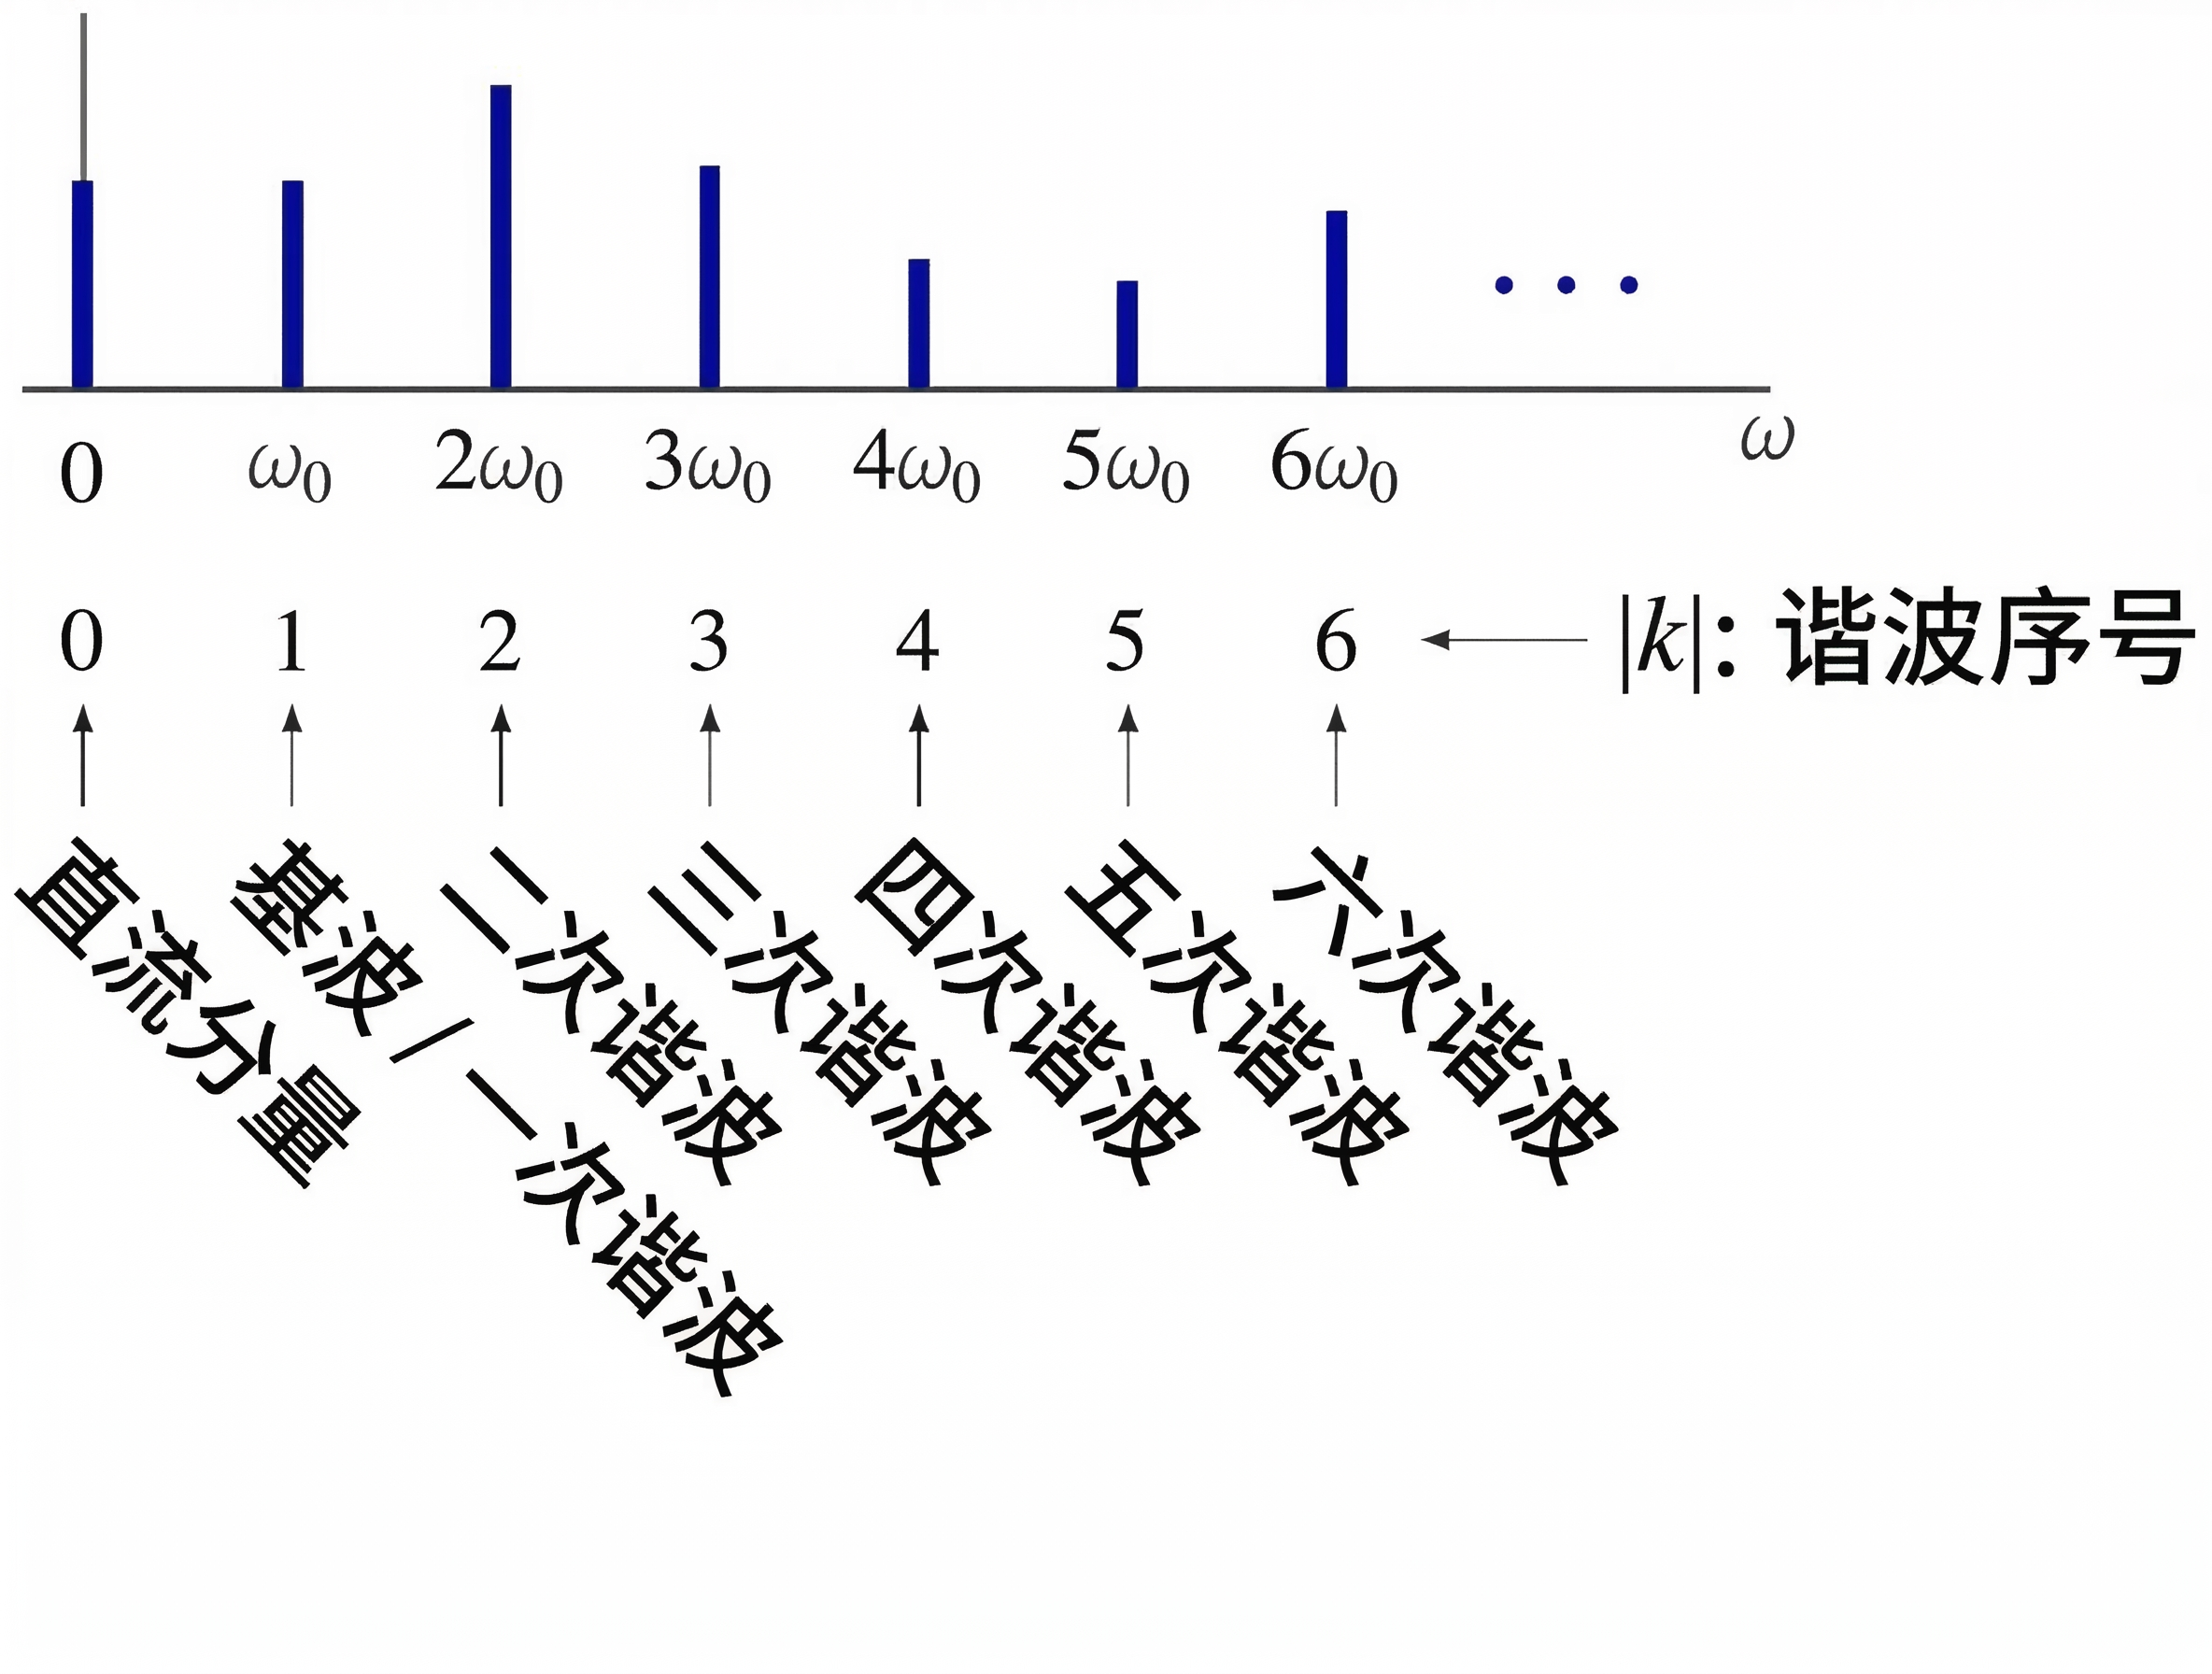
\includegraphics[keepaspectratio]{imglink/Harmonics.png}}
\end{center}
\end{frame}

\begin{frame}{谐波 (Harmonics)}
\protect\phantomsection\label{ux8c10ux6ce2-harmonics-1}
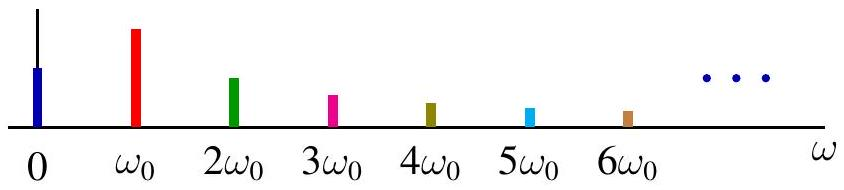
\includegraphics[width=0.55\linewidth,height=\textheight,keepaspectratio]{imglink/42d286b0-1293-4bd1-b498-da763b255ab3-13.png}

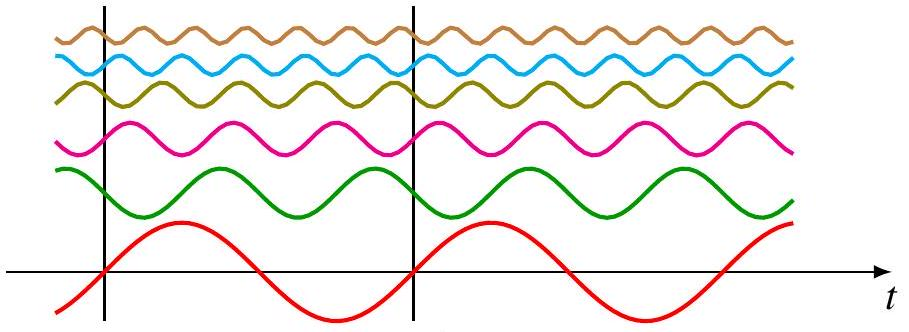
\includegraphics[width=0.55\linewidth,height=\textheight,keepaspectratio]{imglink/42d286b0-1293-4bd1-b498-da763b255ab3-13_3.png}

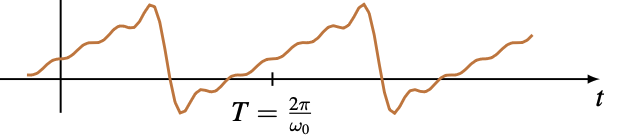
\includegraphics[width=0.58\linewidth,height=\textheight,keepaspectratio]{imglink/Harmonics2.png}
\end{frame}

\begin{frame}{谐波的正交归一性 (Orthonormality)}
\protect\phantomsection\label{ux8c10ux6ce2ux7684ux6b63ux4ea4ux5f52ux4e00ux6027-orthonormality}
回顾对于 \(k \neq 0\)，

\[
\int_{a}^{b} e^{j k \omega_{0} t} d t=\frac{e^{j k \omega_{0} b}-e^{j k \omega_{0} a}}{j k \omega_{0}}
\]

由于 \(e^{j k \omega_{0} t}\) 具有周期 \(T\)，在任意一个周期内：

\[
\frac{1}{T} \int_{T} e^{j k \omega_{0} t} d t=\frac{1}{T} \int_{t_{0}}^{t_{0}+T} e^{j k \omega_{0} t} d t=\delta[k]
\]

定义两个周期为 \(T\) 的信号的\textbf{内积 (inner product)} 为：

\[
\langle f, g\rangle=\frac{1}{T} \int_{T} f(t) \overline{g(t)} d t
\]

\(\left\{e^{j k \omega_{0} t}: k \in \mathbb{Z}\right\}\)
是一个正交归一的函数系：

\[
\left\langle e^{j k \omega_{0} t}, e^{j m \omega_{0} t}\right\rangle=\frac{1}{T} \int_{T} e^{j(k-m) \omega_{0} t} d t=\delta_{k m}=\delta[k-m]
\]
\end{frame}

\begin{frame}{谐波的正交性 (Orthogonality)}
\protect\phantomsection\label{ux8c10ux6ce2ux7684ux6b63ux4ea4ux6027-orthogonality}
对于正弦和余弦函数：

\[
\begin{aligned}
& \left\langle\sin \left(k \omega_{0} t\right), \sin \left(m \omega_{0} t\right)\right\rangle=\frac{1}{2} \delta[k-m]-\frac{1}{2} \delta[k+m] \\
& \left\langle\cos \left(k \omega_{0} t\right), \cos \left(m \omega_{0} t\right)\right\rangle=\frac{1}{2} \delta[k-m]+\frac{1}{2} \delta[k+m] \\
& \left\langle\sin \left(k \omega_{0} t\right), \cos \left(m \omega_{0} t\right)\right\rangle=0
\end{aligned}
\]

\textbf{证明}： 使用欧拉公式和
\(\left\{e^{i k \omega_{0} t}: k \in \mathbb{Z}\right\}\) 的正交归一性。
\end{frame}

\begin{frame}{谐波的正交性 (图示)}
\protect\phantomsection\label{ux8c10ux6ce2ux7684ux6b63ux4ea4ux6027-ux56feux793a}
\[
\begin{gathered}
\sin \left(\omega_{0} t\right) \\
\sin \left(2 \omega_{0} t\right)
\end{gathered}
\]

\begin{center}
\pandocbounded{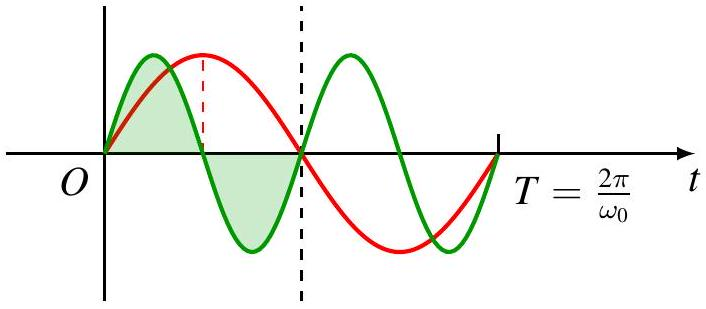
\includegraphics[keepaspectratio]{imglink/42d286b0-1293-4bd1-b498-da763b255ab3-16_2.png}}
\end{center}

\[
\begin{aligned}
& \sin \left(\omega_{0} t\right) \\
& \cos \left(\omega_{0} t\right)
\end{aligned}
\]

\begin{center}
\pandocbounded{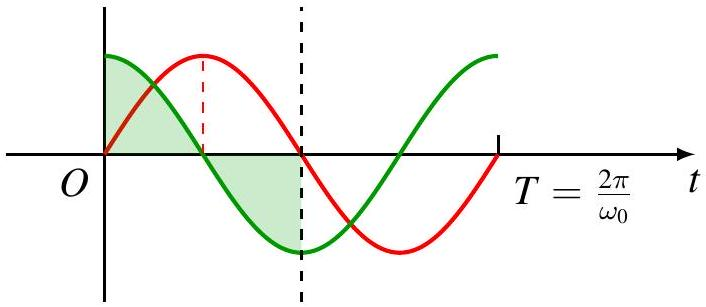
\includegraphics[keepaspectratio]{imglink/42d286b0-1293-4bd1-b498-da763b255ab3-16.png}}
\end{center}
\end{frame}

\begin{frame}{傅里叶系数 (Fourier Coefficients)}
\protect\phantomsection\label{ux5085ux91ccux53f6ux7cfbux6570-fourier-coefficients}
假设 \(x\) 周期为 \(T\) 且有傅里叶级数表示：

\[
x(t)=\sum_{k=-\infty}^{\infty} c_{k} e^{j k \omega_{0} t}, \quad \omega_{0}=\frac{2 \pi}{T}
\]

利用 \(\left\{e^{j k \omega_{0} t}\right\}\)
的正交归一性求解傅里叶系数：

\[
\begin{aligned}
\left\langle x, e^{j m \omega_{0} t}\right\rangle & =\left\langle\sum_{k=-\infty}^{\infty} c_{k} e^{j k \omega_{0} t}, e^{j m \omega_{0} t}\right\rangle \\
& =\sum_{k=-\infty}^{\infty} c_{k}\left\langle e^{j k \omega_{0} t}, e^{j m \omega_{0} t}\right\rangle \\
& =\sum_{k=-\infty}^{\infty} c_{k} \delta[m-k]=c_{m}
\end{aligned}
\]
\end{frame}

\begin{frame}{复数傅里叶级数}
\protect\phantomsection\label{ux590dux6570ux5085ux91ccux53f6ux7ea7ux6570}
\textbf{综合方程 (Synthesis equation)}

\[
x(t)=\sum_{k=-\infty}^{\infty} \hat{x}[k] e^{j k \omega_{0} t}=\sum_{k=-\infty}^{\infty} \hat{x}[k] e^{j k \frac{2 \pi}{T} t}
\]

\(N\) 次部分和： \[
S_{N}(x)(t)=\sum_{k=-N}^{N} \hat{x}[k] e^{i k \omega_{0} t}
\]

\textbf{分析方程 (Analysis equation)}

\[
\hat{x}[k]=\left\langle x, e^{j k \omega_{0} t}\right\rangle=\frac{1}{T} \int_{T} x(t) e^{-j k \omega_{0} t} d t=\frac{1}{T} \int_{T} x(t) e^{-j k \frac{2 \pi}{T} t} d t
\]
\end{frame}

\begin{frame}{三角傅里叶级数}
\protect\phantomsection\label{ux4e09ux89d2ux5085ux91ccux53f6ux7ea7ux6570}
对于正弦和余弦：

\begin{itemize}
\item
  正弦与正弦正交
\item
  余弦与余弦正交
\item
  正弦与余弦正交
\end{itemize}

\textbf{综合方程}

\[
x(t)=a_{0}+\sum_{k=1}^{\infty}\left[a_{k} \cos \left(k \omega_{0} t\right)+b_{k} \sin \left(k \omega_{0} t\right)\right]
\]

\textbf{分析方程}

\[
a_{k}=\frac{2-\delta[k]}{T} \int_{T} x(t) \cos \left(k \omega_{0} t\right) d t, \quad b_{k}=\frac{2}{T} \int_{T} x(t) \sin \left(k \omega_{0} t\right) d t
\]
\end{frame}

\begin{frame}{两种形式的等价性}
\protect\phantomsection\label{ux4e24ux79cdux5f62ux5f0fux7684ux7b49ux4ef7ux6027}
\textbf{复数形式} \[
x(t)=\sum_{k=-\infty}^{\infty} \hat{x}[k] e^{j k \omega_{0} t}
\]

\textbf{三角形式} \[
x(t)=a_{0}+\sum_{k=1}^{\infty}\left[a_{k} \cos \left(k \omega_{0} t\right)+b_{k} \sin \left(k \omega_{0} t\right)\right]
\]

\textbf{系数转换 (通过欧拉公式)}

\[
\left\{\begin{array}{ll}
a_{0}=\hat{x}[0] \\
a_{k}=\hat{x}[k]+\hat{x}[-k], \\
b_{k}=j(\hat{x}[k]-\hat{x}[-k]),
\end{array} \quad k \geq 1 \quad  \begin{cases}\hat{x}[0]=a_{0} \\
\hat{x}[k]=\frac{1}{2}\left(a_{k}-j b_{k}\right), & k \geq 1 \\
\hat{x}[k]=\frac{1}{2}\left(a_{k}+j b_{-k}\right), & k \leq-1\end{cases}\right.
\]

复数形式中的负频率是为了数学上的方便引入的，没有直接的物理意义。
\end{frame}

\begin{frame}{例子}
\protect\phantomsection\label{ux4f8bux5b50}
例子：\(x(t)=e^{j \omega_{0} t}, \hat{x}[k]=\delta[k-1]\)

\begin{columns}[T]
\begin{column}{0.5\linewidth}
频谱 \(\hat{x}[k]\)
\end{column}

\begin{column}{0.5\linewidth}
\pandocbounded{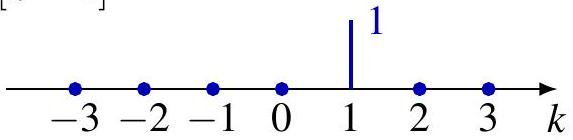
\includegraphics[keepaspectratio]{imglink/42d286b0-1293-4bd1-b498-da763b255ab3-21_2.png}}
\end{column}
\end{columns}

例子：\(x(t)=\cos \left(\omega_{0} t+\phi\right)=\frac{e^{i \phi}}{2} e^{j \omega_{0} t}+\frac{e^{-j \phi}}{2} e^{-j \omega_{0} t}\)，

显然： \[
\hat{x}[1]=\frac{1}{2} e^{j \phi}, \quad, \hat{x}[-1]=\frac{1}{2} e^{-j \phi}, \quad \hat{x}[k]=0, k \neq \pm 1
\]

\begin{columns}[T]
\begin{column}{0.5\linewidth}
幅值谱 \(|\hat{x}[k]|\)

相位谱 \(\arg \hat{x}[k]\)
\end{column}

\begin{column}{0.5\linewidth}
\pandocbounded{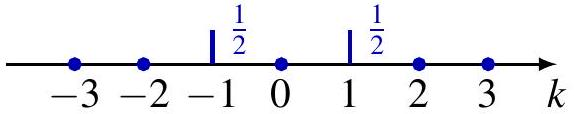
\includegraphics[keepaspectratio]{imglink/42d286b0-1293-4bd1-b498-da763b255ab3-21.png}}

\pandocbounded{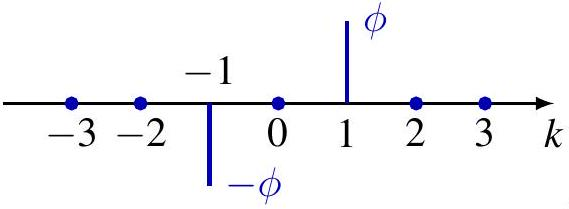
\includegraphics[keepaspectratio]{imglink/42d286b0-1293-4bd1-b498-da763b255ab3-21_3.png}}
\end{column}
\end{columns}
\end{frame}

\begin{frame}{例子：三角波 (Triangle Wave)}
\protect\phantomsection\label{ux4f8bux5b50ux4e09ux89d2ux6ce2-triangle-wave}
在一个周期内，

\[
x(t)=1-\frac{2|t|}{T}, \quad|t| \leq \frac{T}{2}
\]

\pandocbounded{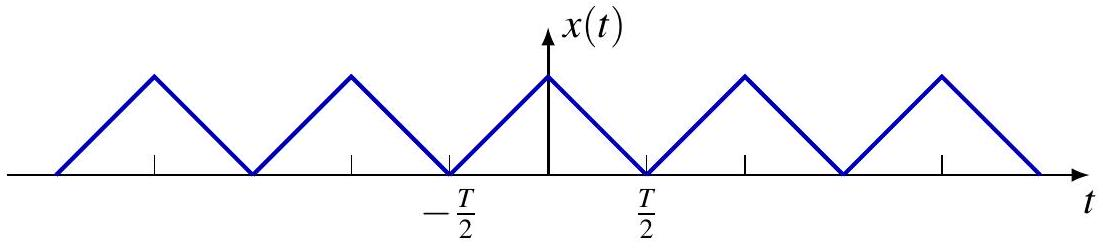
\includegraphics[keepaspectratio]{imglink/42d286b0-1293-4bd1-b498-da763b255ab3-22.png}}

傅里叶系数：

\[
k=0, \quad \hat{x}[0]=\frac{1}{T} \int_{-T / 2}^{T / 2}\left(1-\frac{2|t|}{T}\right) d t=\frac{1}{2}
\]

\(k \neq 0, k\)
为奇数,\(\quad \hat{x}[k]=\frac{1}{T} \int_{-T / 2}^{T / 2}\left(1-\frac{2|t|}{T}\right) e^{-j k \omega_{0} t} d t=\frac{2}{\pi^{2} k^{2}}\)
\(k \neq 0, k\) 为偶数, \(\quad \hat{x}[k]=0\)
\end{frame}

\begin{frame}{例子：三角波频谱}
\protect\phantomsection\label{ux4f8bux5b50ux4e09ux89d2ux6ce2ux9891ux8c31}
\[
\hat{x}[k]= \begin{cases}\frac{1}{2}, & k=0 \\ \frac{2}{\pi^{2} k^{2}}, & k \neq 0 \text { 奇数 } \\ 0, & k \neq 0 \text { 偶数 }\end{cases}
\]

固定 \(T\) 的频谱，频率间隔
\(\Delta \omega=\frac{2 \pi}{T}， \omega_{k}=k \frac{2 \pi}{T}\)

\begin{center}
\pandocbounded{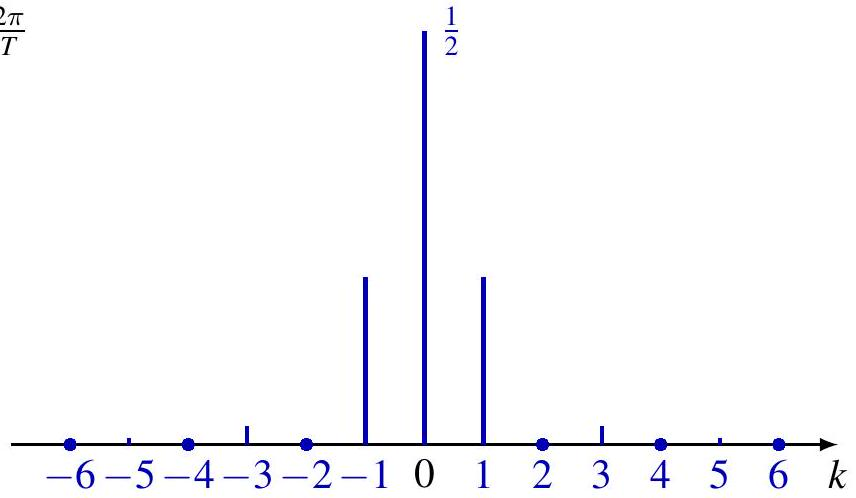
\includegraphics[keepaspectratio]{imglink/42d286b0-1293-4bd1-b498-da763b255ab3-23.png}}
\end{center}
\end{frame}

\begin{frame}{例子：三角波合成 (\(N=0\))}
\protect\phantomsection\label{ux4f8bux5b50ux4e09ux89d2ux6ce2ux5408ux6210-n0}
\[
S_{0}(x)(t)=\sum_{k=-0}^{0} \hat{x}[k] e^{j k \omega_{0} t}
\]

\pandocbounded{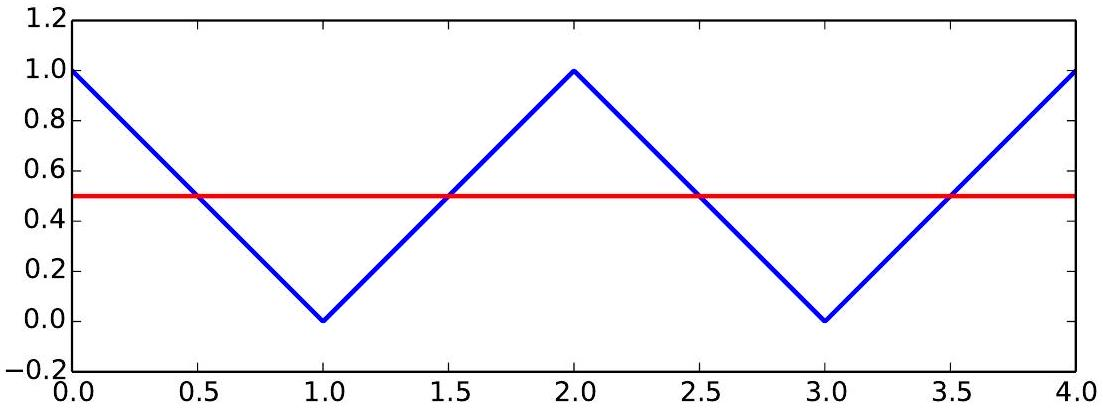
\includegraphics[keepaspectratio]{imglink/42d286b0-1293-4bd1-b498-da763b255ab3-24.png}}
\end{frame}

\begin{frame}{例子：三角波合成 (\(N=1\))}
\protect\phantomsection\label{ux4f8bux5b50ux4e09ux89d2ux6ce2ux5408ux6210-n1}
\[
S_{1}(x)(t)=\sum_{k=-1}^{1} \hat{x}[k] e^{j k \omega_{0} t}
\]

\pandocbounded{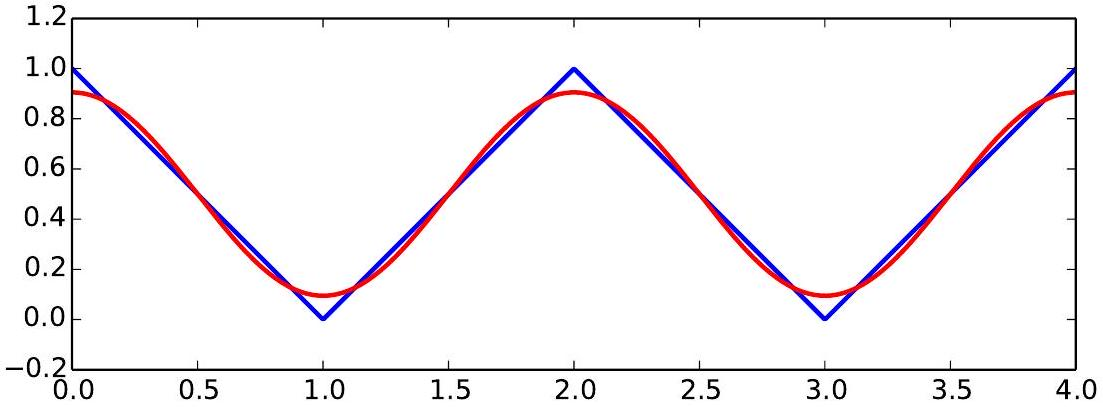
\includegraphics[keepaspectratio]{imglink/42d286b0-1293-4bd1-b498-da763b255ab3-25.png}}
\end{frame}

\begin{frame}{例子：三角波合成 (\(N=3\))}
\protect\phantomsection\label{ux4f8bux5b50ux4e09ux89d2ux6ce2ux5408ux6210-n3}
\[
S_{3}(x)(t)=\sum_{k=-3}^{3} \hat{x}[k] e^{j k \omega_{0} t}
\]

\pandocbounded{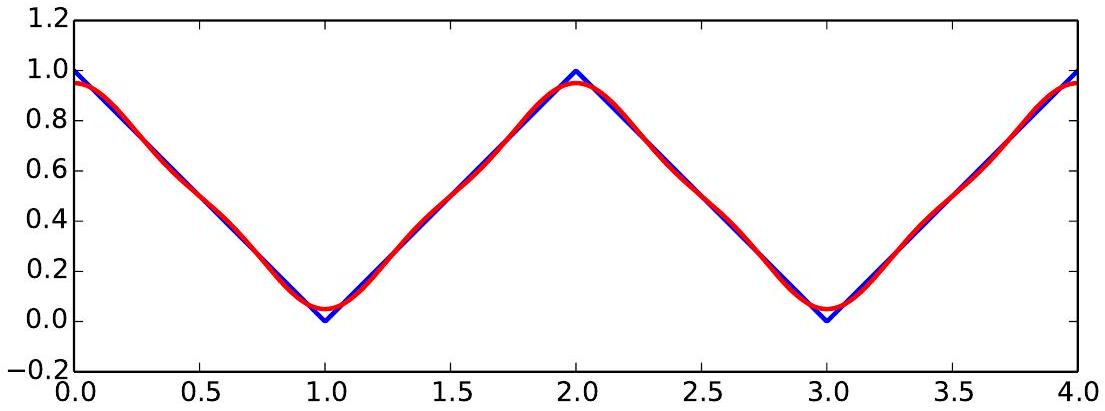
\includegraphics[keepaspectratio]{imglink/42d286b0-1293-4bd1-b498-da763b255ab3-26.png}}
\end{frame}

\begin{frame}{例子：三角波合成 (\(N=5\))}
\protect\phantomsection\label{ux4f8bux5b50ux4e09ux89d2ux6ce2ux5408ux6210-n5}
\[
S_{5}(x)(t)=\sum_{k=-5}^{5} \hat{x}[k] e^{j k \omega_{0} t}
\]

\pandocbounded{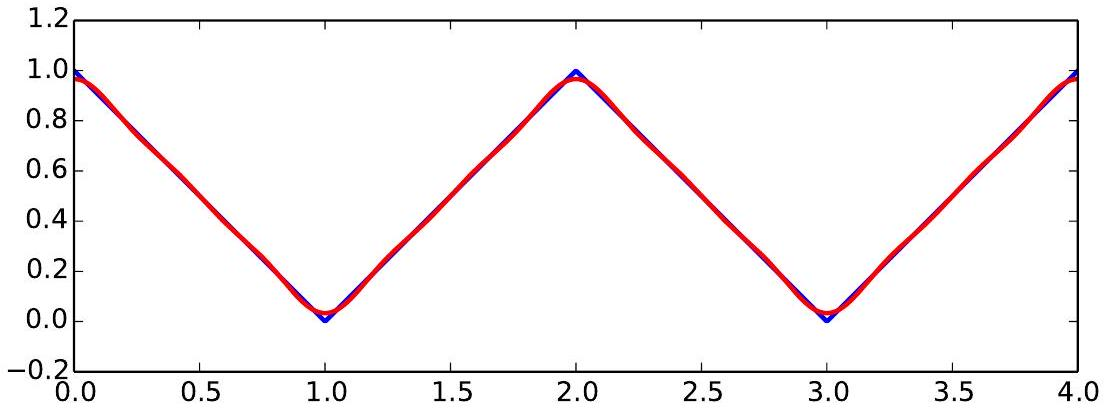
\includegraphics[keepaspectratio]{imglink/42d286b0-1293-4bd1-b498-da763b255ab3-27.png}}
\end{frame}

\begin{frame}{例子：三角波合成 (\(N=7\))}
\protect\phantomsection\label{ux4f8bux5b50ux4e09ux89d2ux6ce2ux5408ux6210-n7}
\[
S_{7}(x)(t)=\sum_{k=-7}^{7} \hat{x}[k] e^{j k \omega_{0} t}
\]

\pandocbounded{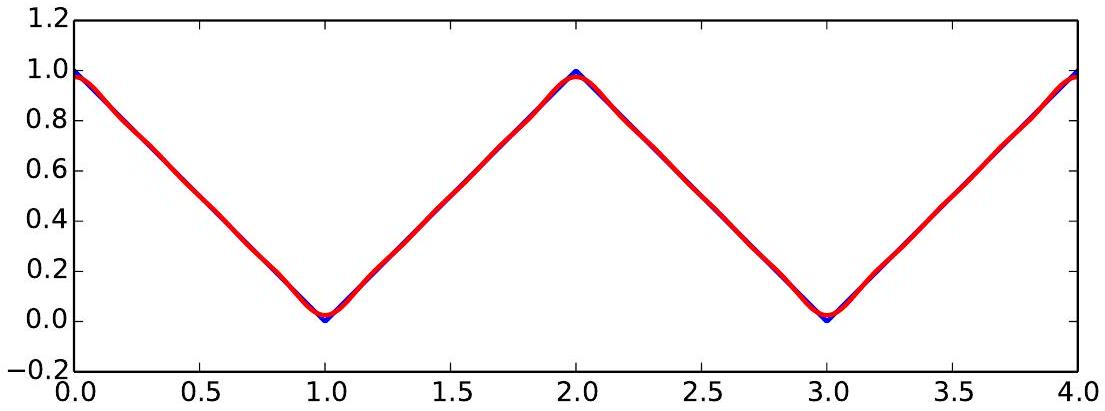
\includegraphics[keepaspectratio]{imglink/42d286b0-1293-4bd1-b498-da763b255ab3-28.png}}
\end{frame}

\begin{frame}{例子：三角波合成 (\(N=9\))}
\protect\phantomsection\label{ux4f8bux5b50ux4e09ux89d2ux6ce2ux5408ux6210-n9}
\[
S_{9}(x)(t)=\sum_{k=-9}^{9} \hat{x}[k] e^{j k \omega_{0} t}
\]

\pandocbounded{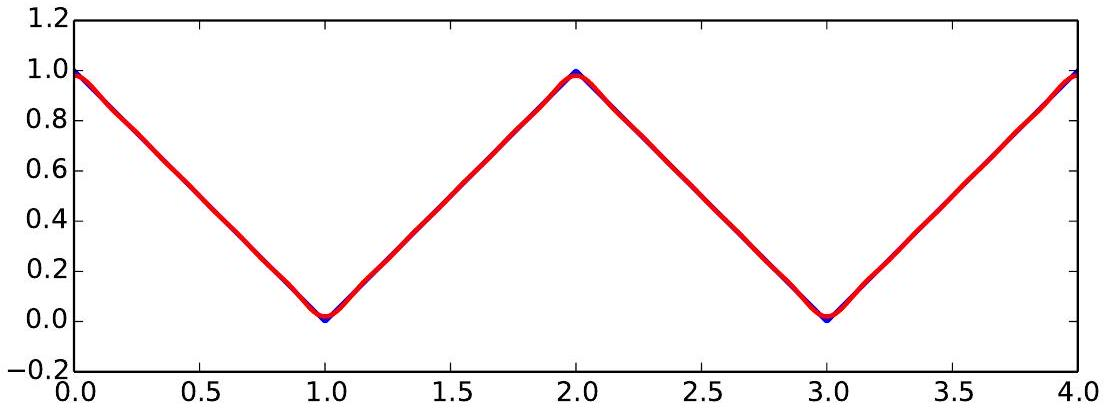
\includegraphics[keepaspectratio]{imglink/42d286b0-1293-4bd1-b498-da763b255ab3-29.png}}
\end{frame}

\begin{frame}{例子：三角波合成 (\(N=19\))}
\protect\phantomsection\label{ux4f8bux5b50ux4e09ux89d2ux6ce2ux5408ux6210-n19}
\[
S_{19}(x)(t)=\sum_{k=-19}^{19} \hat{x}[k] e^{j k \omega_{0} t}
\]

\pandocbounded{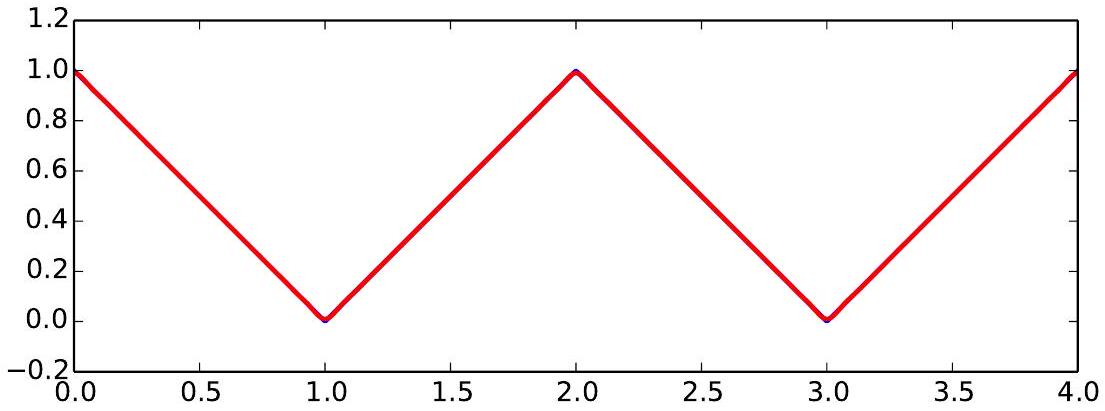
\includegraphics[keepaspectratio]{imglink/42d286b0-1293-4bd1-b498-da763b255ab3-30.png}}
\end{frame}

\begin{frame}{例子：周期方波 (Periodic Square Wave)}
\protect\phantomsection\label{ux4f8bux5b50ux5468ux671fux65b9ux6ce2-periodic-square-wave}
在一个周期内，

\[
x(t)= \begin{cases}1, & |t|<T_{1} \\ 0, & T_{1}<|t|<T / 2\end{cases}
\]

\pandocbounded{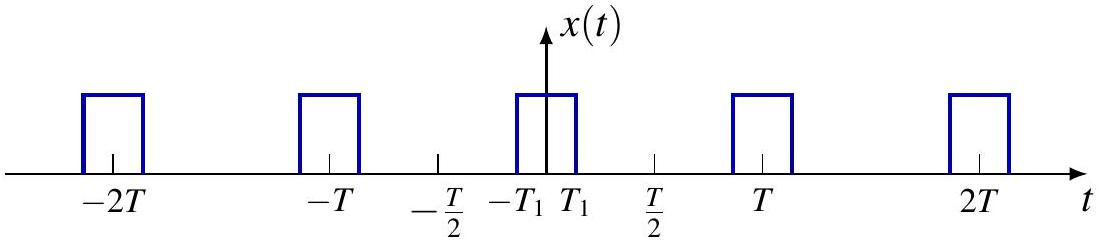
\includegraphics[keepaspectratio]{imglink/42d286b0-1293-4bd1-b498-da763b255ab3-31.png}}

傅里叶系数：

\[
\begin{array}{ll}
k=0, & \hat{x}[0]=\frac{1}{T} \int_{-T_{1}}^{T_{1}} 1 d t=\frac{2 T_{1}}{T} \\
k \neq 0, & \hat{x}[k]=\frac{1}{T} \int_{-T_{1}}^{T_{1}} e^{-j k \omega_{0} t} d t=\frac{2 \sin \left(k \omega_{0} T_{1}\right)}{k \omega_{0} T}=\frac{\sin \left(k \omega_{0} T_{1}\right)}{k \pi}
\end{array}
\]
\end{frame}

\begin{frame}{例子：周期方波频谱}
\protect\phantomsection\label{ux4f8bux5b50ux5468ux671fux65b9ux6ce2ux9891ux8c31}
\[
\hat{x}[k]=\frac{\sin \left(k \frac{2 \pi T_{1}}{T}\right)}{k \pi}=\frac{2 \sin \left(\omega_{k} T_{1}\right)}{\omega_{k} T}
\]

固定 \(T\)，不同 \(T_{1}\) 的频谱：

\begin{columns}[T]
\begin{column}{0.05\linewidth}
\end{column}

\begin{column}{0.9\linewidth}
\pandocbounded{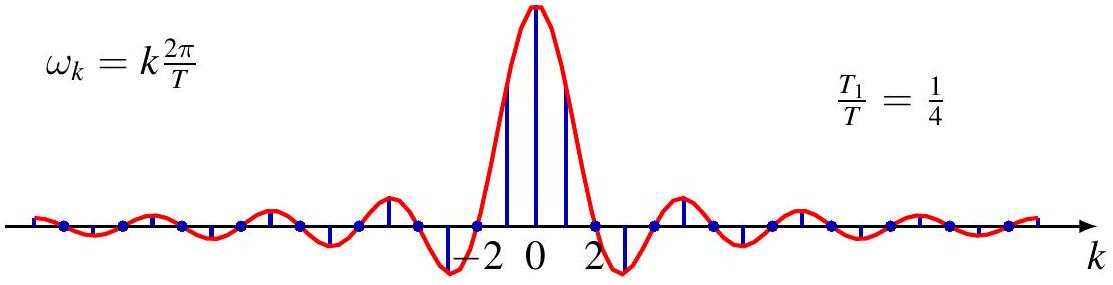
\includegraphics[keepaspectratio]{imglink/42d286b0-1293-4bd1-b498-da763b255ab3-32_3.png}}

\pandocbounded{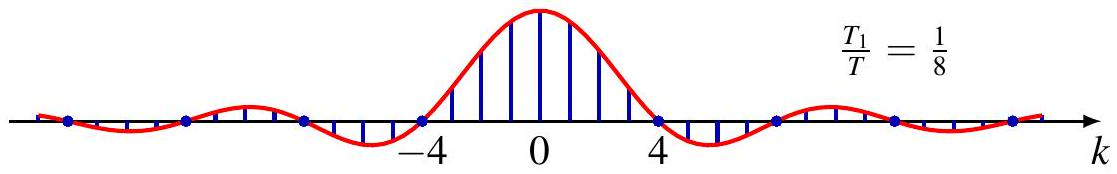
\includegraphics[keepaspectratio]{imglink/42d286b0-1293-4bd1-b498-da763b255ab3-32_2.png}}

\pandocbounded{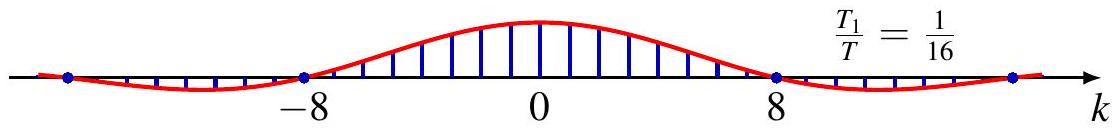
\includegraphics[keepaspectratio]{imglink/42d286b0-1293-4bd1-b498-da763b255ab3-32.png}}
\end{column}

\begin{column}{0.05\linewidth}
\end{column}
\end{columns}
\end{frame}

\begin{frame}{例子：周期方波频谱 (不同 \(T\))}
\protect\phantomsection\label{ux4f8bux5b50ux5468ux671fux65b9ux6ce2ux9891ux8c31-ux4e0dux540c-t}
\[
\hat{x}[k]=\frac{\sin \left(k \frac{2 \pi T_{1}}{T}\right)}{k \pi}=\frac{2 \sin \left(\omega_{k} T_{1}\right)}{\omega_{k} T}
\]

固定 \(T_{1}\)，不同 \(T\) 的频谱：

\begin{columns}[T]
\begin{column}{0.05\linewidth}
\end{column}

\begin{column}{0.9\linewidth}
\pandocbounded{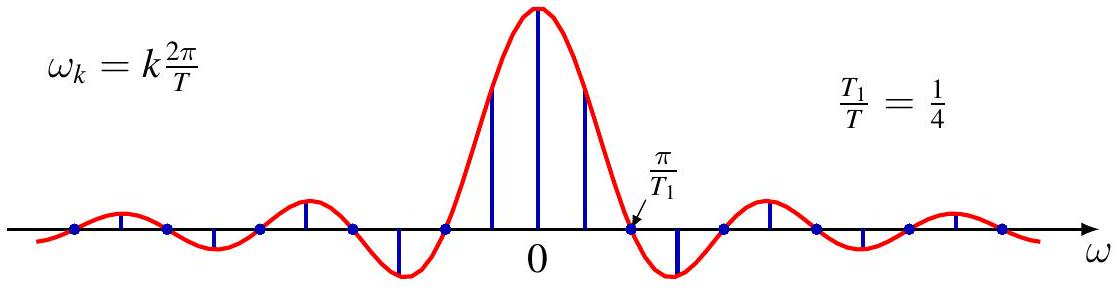
\includegraphics[keepaspectratio]{imglink/42d286b0-1293-4bd1-b498-da763b255ab3-33_3.png}}

\pandocbounded{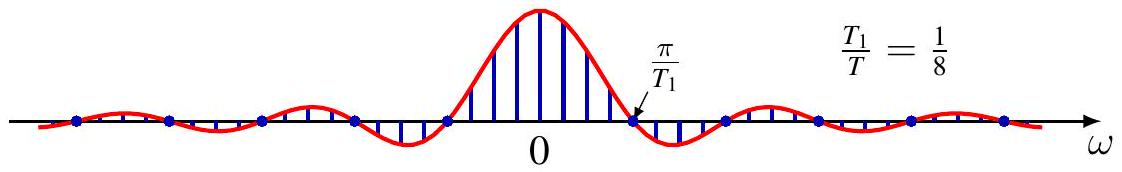
\includegraphics[keepaspectratio]{imglink/42d286b0-1293-4bd1-b498-da763b255ab3-33_2.png}}

\pandocbounded{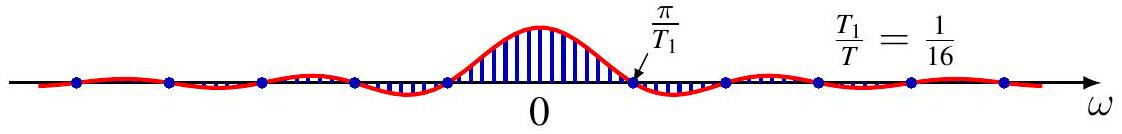
\includegraphics[keepaspectratio]{imglink/42d286b0-1293-4bd1-b498-da763b255ab3-33.png}}
\end{column}

\begin{column}{0.05\linewidth}
\end{column}
\end{columns}
\end{frame}

\begin{frame}{例子：方波合成 (\(N=0\))}
\protect\phantomsection\label{ux4f8bux5b50ux65b9ux6ce2ux5408ux6210-n0}
\[
S_{0}(x)(t)=\sum_{k=-0}^{0} \hat{x}[k] e^{j k \omega_{0} t}
\]

\begin{center}
\pandocbounded{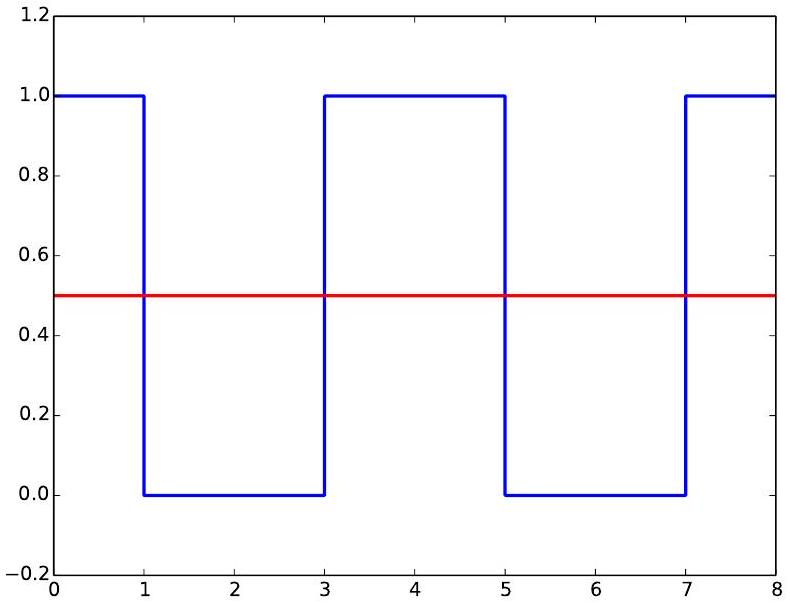
\includegraphics[keepaspectratio]{imglink/42d286b0-1293-4bd1-b498-da763b255ab3-34.png}}
\end{center}
\end{frame}

\begin{frame}{例子：方波合成 (\(N=1\))}
\protect\phantomsection\label{ux4f8bux5b50ux65b9ux6ce2ux5408ux6210-n1}
\[
S_{1}(x)(t)=\sum_{k=-1}^{1} \hat{x}[k] e^{j k \omega_{0} t}
\]

\begin{center}
\pandocbounded{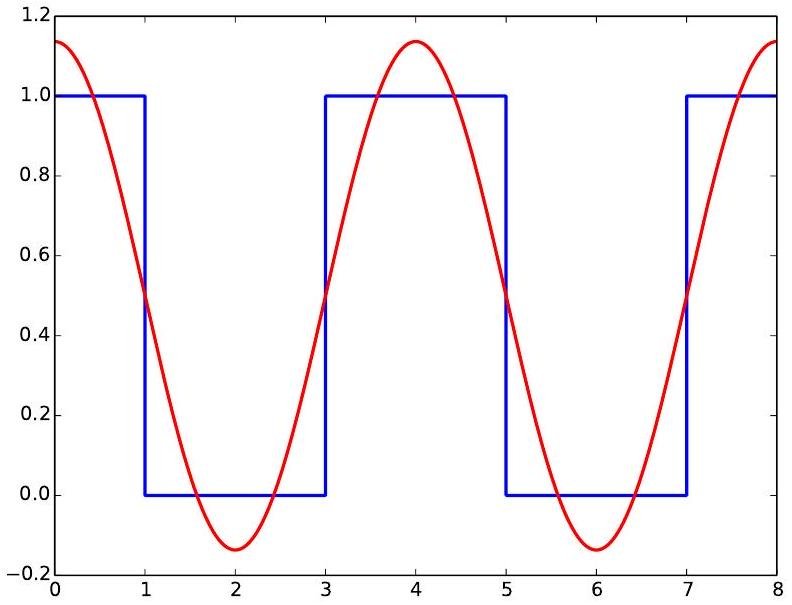
\includegraphics[keepaspectratio]{imglink/42d286b0-1293-4bd1-b498-da763b255ab3-35.png}}
\end{center}
\end{frame}

\begin{frame}{例子：方波合成 (\(N=3\))}
\protect\phantomsection\label{ux4f8bux5b50ux65b9ux6ce2ux5408ux6210-n3}
\[
S_{3}(x)(t)=\sum_{k=-3}^{3} \hat{x}[k] e^{j k \omega_{0} t}
\]

\begin{center}
\pandocbounded{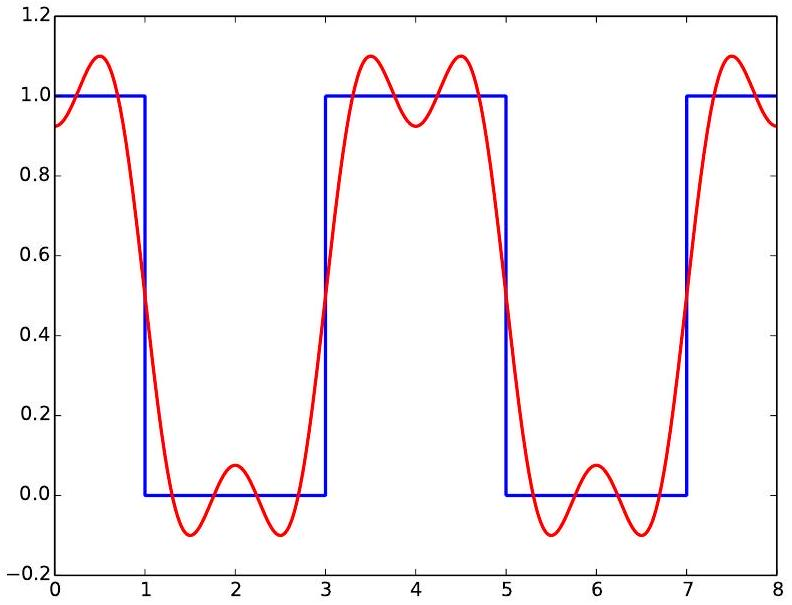
\includegraphics[keepaspectratio]{imglink/42d286b0-1293-4bd1-b498-da763b255ab3-36.png}}
\end{center}
\end{frame}

\begin{frame}{例子：方波合成 (\(N=5\))}
\protect\phantomsection\label{ux4f8bux5b50ux65b9ux6ce2ux5408ux6210-n5}
\[
S_{5}(x)(t)=\sum_{k=-5}^{5} \hat{x}[k] e^{j k \omega_{0} t}
\]

\begin{center}
\pandocbounded{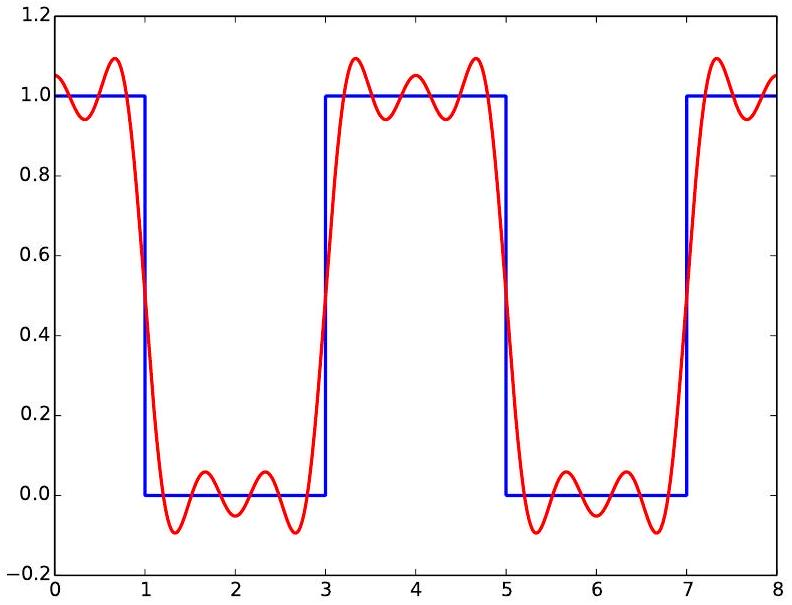
\includegraphics[keepaspectratio]{imglink/42d286b0-1293-4bd1-b498-da763b255ab3-37.png}}
\end{center}
\end{frame}

\begin{frame}{例子：方波合成 (\(N=7\))}
\protect\phantomsection\label{ux4f8bux5b50ux65b9ux6ce2ux5408ux6210-n7}
\[
S_{7}(x)(t)=\sum_{k=-7}^{7} \hat{x}[k] e^{j k \omega_{0} t}
\]

\begin{center}
\pandocbounded{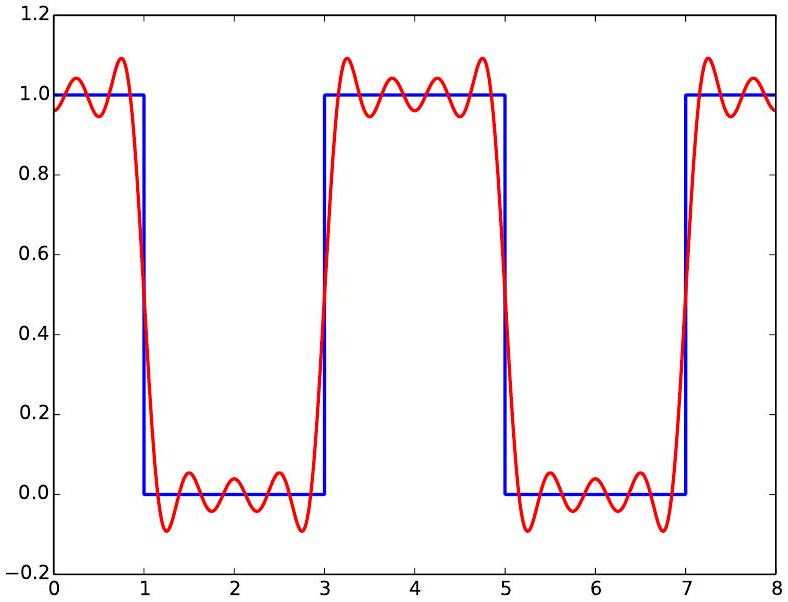
\includegraphics[keepaspectratio]{imglink/42d286b0-1293-4bd1-b498-da763b255ab3-38.png}}
\end{center}
\end{frame}

\begin{frame}{例子：方波合成 (\(N=9\))}
\protect\phantomsection\label{ux4f8bux5b50ux65b9ux6ce2ux5408ux6210-n9}
\[
S_{9}(x)(t)=\sum_{k=-9}^{9} \hat{x}[k] e^{j k \omega_{0} t}
\]

\begin{center}
\pandocbounded{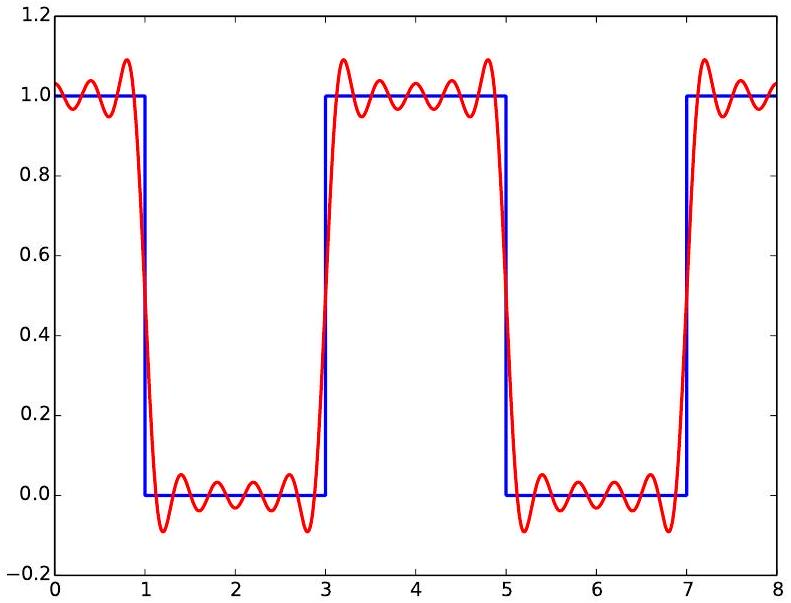
\includegraphics[keepaspectratio]{imglink/42d286b0-1293-4bd1-b498-da763b255ab3-39.png}}
\end{center}
\end{frame}

\begin{frame}{例子：方波合成 (\(N=13\))}
\protect\phantomsection\label{ux4f8bux5b50ux65b9ux6ce2ux5408ux6210-n13}
\[
S_{13}(x)(t)=\sum_{k=-13}^{13} \hat{x}[k] e^{j k \omega_{0} t}
\]

\begin{center}
\pandocbounded{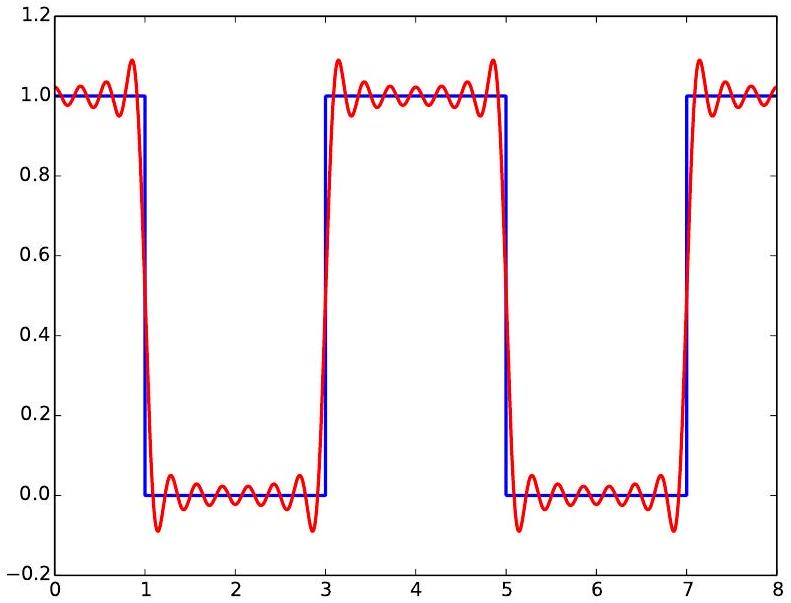
\includegraphics[keepaspectratio]{imglink/42d286b0-1293-4bd1-b498-da763b255ab3-40.png}}
\end{center}
\end{frame}

\begin{frame}{例子：方波合成 (\(N=19\))}
\protect\phantomsection\label{ux4f8bux5b50ux65b9ux6ce2ux5408ux6210-n19}
\[
S_{19}(x)(t)=\sum_{k=-19}^{19} \hat{x}[k] e^{j k \omega_{0} t}
\]

\begin{center}
\pandocbounded{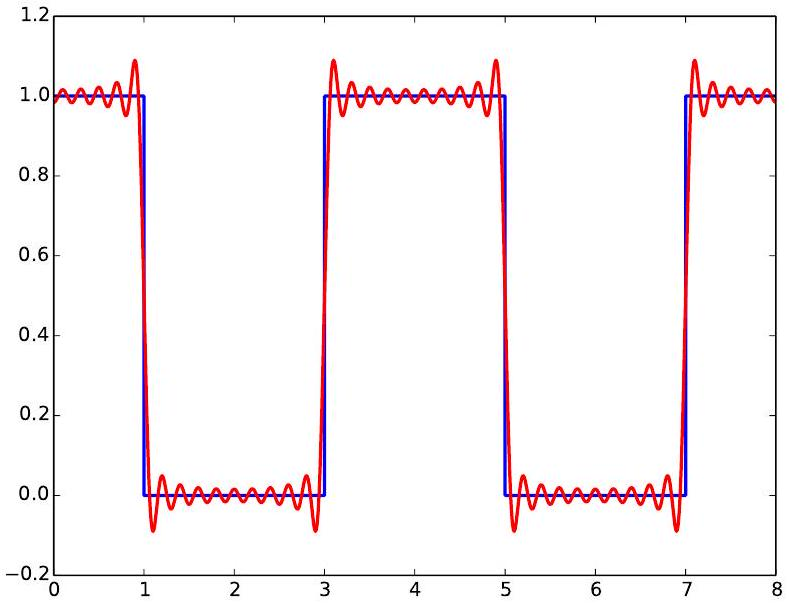
\includegraphics[keepaspectratio]{imglink/42d286b0-1293-4bd1-b498-da763b255ab3-41.png}}
\end{center}
\end{frame}

\begin{frame}{例子：方波合成 (\(N=29\))}
\protect\phantomsection\label{ux4f8bux5b50ux65b9ux6ce2ux5408ux6210-n29}
\[
S_{29}(x)(t)=\sum_{k=-29}^{29} \hat{x}[k] e^{j k \omega_{0} t}
\]

\begin{center}
\pandocbounded{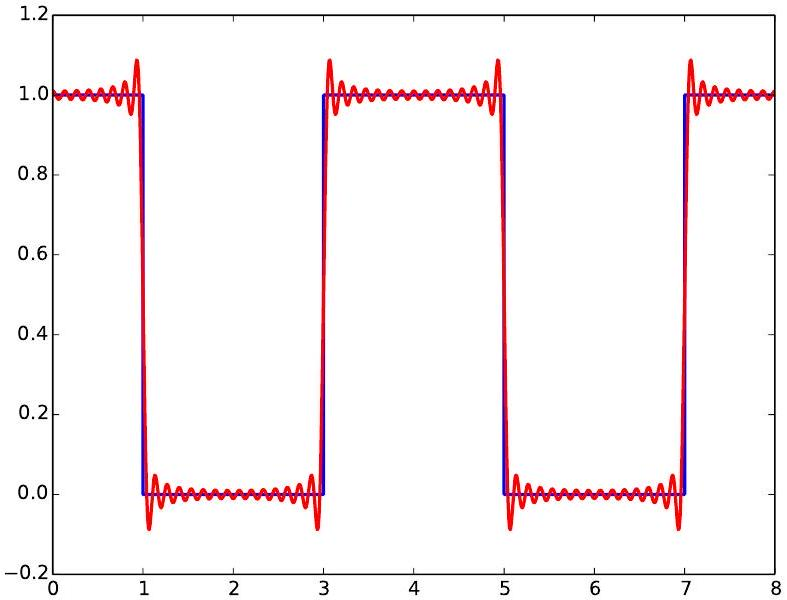
\includegraphics[keepaspectratio]{imglink/42d286b0-1293-4bd1-b498-da763b255ab3-42.png}}
\end{center}
\end{frame}

\begin{frame}{例子：方波合成 (\(N=39\))}
\protect\phantomsection\label{ux4f8bux5b50ux65b9ux6ce2ux5408ux6210-n39}
\[
S_{39}(x)(t)=\sum_{k=-39}^{39} \hat{x}[k] e^{j k \omega_{0} t}
\]

\begin{center}
\pandocbounded{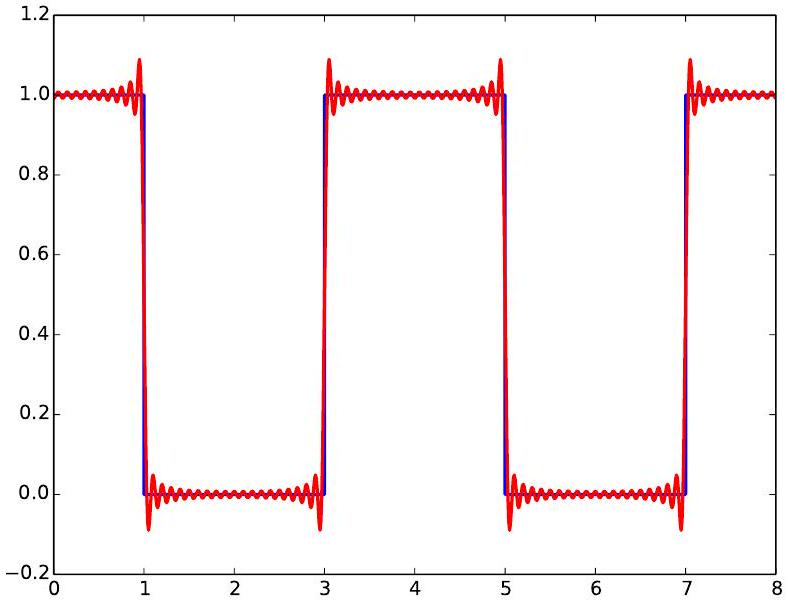
\includegraphics[keepaspectratio]{imglink/42d286b0-1293-4bd1-b498-da763b255ab3-43.png}}
\end{center}
\end{frame}

\begin{frame}{吉布斯现象 (Gibbs Phenomenon)}
\protect\phantomsection\label{ux5409ux5e03ux65afux73b0ux8c61-gibbs-phenomenon}
傅里叶级数的部分和在跳变间断点处``振铃''

\begin{itemize}
\tightlist
\item
  随着项数增加，过冲越来越靠近间断点
\item
  过冲幅度趋近于跳变幅度的 \(\approx 9 \%\)
\end{itemize}

\pandocbounded{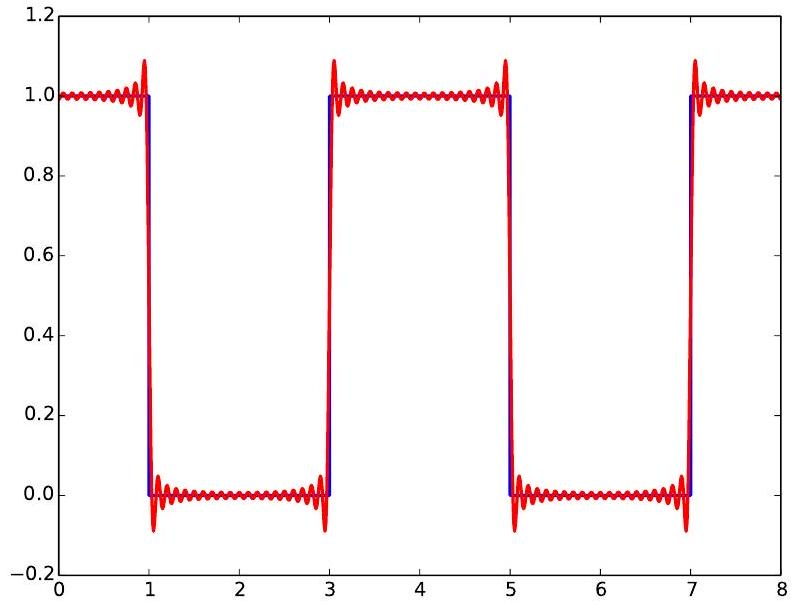
\includegraphics[keepaspectratio]{imglink/42d286b0-1293-4bd1-b498-da763b255ab3-44.png}}
\end{frame}

\begin{frame}{目录}
\protect\phantomsection\label{toc2}
\begin{itemize}
\tightlist
\item
  \hyperlink{sec31}{1. 线性时不变系统对复指数信号的响应}
\item
  \hyperlink{sec32}{2. 连续时间周期信号的傅里叶级数表示}
\item
  \hyperlink{sec33}{\textbf{3. 连续时间傅里叶级数的收敛}}
\item
  \hyperlink{sec34}{4. 连续时间傅里叶级数的性质}
\item
  \hyperlink{35}{5. 离散时间周期信号的傅里叶级数表示}
\item
  \hyperlink{sec36}{6. 离散时间傅里叶级数的性质}
\item
  \hyperlink{sec37}{7. 傅里叶级数与线性时不变系统}
\item
  \hyperlink{sec38}{8. 滤波}

  \begin{itemize}
  \tightlist
  \item
    \hyperlink{sec381}{频率成形滤波器}
  \item
    \hyperlink{sec382}{频率选择性滤波器}
  \item
    \hyperlink{sec383}{用微分方程描述的连续时间滤波器}
  \item
    \hyperlink{sec383}{用差分方程描述的离散时间滤波器}
  \end{itemize}
\end{itemize}
\end{frame}

\section{3. 连续时间傅里叶级数的收敛}\label{sec33}

\begin{frame}{帕塞瓦尔恒等式 (帕塞瓦尔公式，Parseval's Identity)}
\protect\phantomsection\label{ux5e15ux585eux74e6ux5c14ux6052ux7b49ux5f0f-ux5e15ux585eux74e6ux5c14ux516cux5f0fparsevals-identity}
对于具有有限 \textbf{2-范数} 的信号的傅里叶系数：

\[
\sum_{k=-\infty}^{\infty}|\hat{x}[k]|^{2}=\|x\|^{2}=\frac{1}{T} \int_{T}|x(t)|^{2} d t
\] 解释：能量守恒

\begin{itemize}
\tightlist
\item
  \(|\hat{x}[k]|^{2}\) 是第 \(k\) 次谐波分量的平均功率
\item
  \(\|x\|^{2}\) 是 \(x\) 的平均功率
\item
  总功率是所有分量功率之和
\end{itemize}

定理：傅里叶级数在均方意义下收敛

\[
\lim _{N \rightarrow \infty}\left\|x-S_{N}(x)\right\|=0
\]

注意：均方收敛并不意味着逐点收敛。

如何证明？
\end{frame}

\begin{frame}{内积空间中的正交归一系}
\protect\phantomsection\label{ux5185ux79efux7a7aux95f4ux4e2dux7684ux6b63ux4ea4ux5f52ux4e00ux7cfb}
如果 \(\langle x, y\rangle=0\)，则两个向量 \(x, y \in V\)
是\textbf{正交}的。 如果 \(\|x\|=1\) 或
\(\langle x, x\rangle=1\)，则向量 \(x \in V\) 是\textbf{单位向量}。
如果对于 \(m \neq k\)，\(\left\langle x_{k}, x_{m}\right\rangle=0\)，则
\(\left\{x_{k}\right\}\) 是\textbf{正交系}。 如果
\(\left\langle e_{k}, e_{m}\right\rangle=\delta_{k m}=\delta[k-m]\)，则
\(\left\{e_{k}\right\}\) 是\textbf{正交归一系 (orthonormal system)}。

令 \(e_{k}(t)=e^{j k \frac{2 \pi}{T} t}\)。回顾
\(\left\{e_{k}: k \in \mathbb{Z}\right\}\) 是正交归一系：

\[
\left\langle e_{k}, e_{m}\right\rangle=\delta[k-m]
\]

给定正交归一系 \(\left\{e_{k}\right\}\)，假设

\[
x=\sum_{k} c_{k} e_{k}
\]

通过与 \(e_{m}\) 做内积来求系数：

\[
\left\langle x, e_{m}\right\rangle=\left\langle\sum_{k} c_{k} e_{k}, e_{m}\right\rangle=\sum_{k} c_{k}\left\langle e_{k}, e_{m}\right\rangle=\sum_{k} c_{k} \delta[k-m]=c_{m}
\]

广义傅里叶级数：

\[
x=\sum_{k}\left\langle x, e_{k}\right\rangle e_{k}
\]

这就是我们要做的傅里叶级数展开。
\end{frame}

\begin{frame}{最佳均方逼近 (Best Mean-square Approximation)}
\protect\phantomsection\label{ux6700ux4f73ux5747ux65b9ux903cux8fd1-best-mean-square-approximation}
用 \(\operatorname{span}\left\{e_{1}, \ldots, e_{n}\right\}\)
中的元素逼近 \(x\) 的均方误差，即用形式为
\(y=\sum_{k=1}^{n} a_{k} e_{k}\) 的元素：

\[
\begin{aligned}
\|x-y\|^{2} & =\left\langle x-\sum_{k=1}^{n} a_{k} e_{k}, x-\sum_{k=1}^{n} a_{k} e_{k}\right\rangle \\
& =\|x\|^{2}-\sum_{k=1}^{n} a_{k}\left\langle e_{k}, x\right\rangle-\sum_{k=1}^{n} \bar{a}_{k}\left\langle x, e_{k}\right\rangle+\sum_{k=1}^{n}\left|a_{k}\right|^{2} \\
& =\|x\|^{2}-2 \sum_{k=1}^{n} \operatorname{Re}\left(\bar{a}_{k}\left\langle x, e_{k}\right\rangle\right)+\sum_{k=1}^{n}\left|a_{k}\right|^{2} \\
& \geq\|x\|^{2}-2 \sum_{k=1}^{n}\left|a_{k}\right| \cdot\left|\left\langle x, e_{k},\right\rangle\right|+\sum_{k=1}^{n}\left|a_{k}\right|^{2} \quad(\text { 使用 }|\operatorname{Re} z| \leq|z|) \\
& =\|x\|^{2}-\sum_{k=1}^{n}\left|\left\langle x, e_{k}\right\rangle\right|^{2}+\sum_{k=1}^{n}\left(\left|a_{k}\right|-\left|\left\langle x, e_{k},\right\rangle\right|\right)^{2}
\end{aligned}
\]
\end{frame}

\begin{frame}{最佳均方逼近 (续)}
\protect\phantomsection\label{ux6700ux4f73ux5747ux65b9ux903cux8fd1-ux7eed}
逼近的均方误差：

\[
\begin{aligned}
\|x-y\|^{2} & \stackrel{(1)}{\geq}\|x\|^{2}-\sum_{k=1}^{n}\left|\left\langle x, e_{k}\right\rangle\right|^{2}+\sum_{k=1}^{n}\left(\left|a_{k}\right|-\left|\left\langle x, e_{k},\right\rangle\right|\right)^{2} \\
& \stackrel{(2)}{\geq}\|x\|^{2}-\sum_{k=1}^{n}\left|\left\langle x, e_{k}\right\rangle\right|^{2}
\end{aligned}
\]

当且仅当 \(a_{k}=\left\langle x, e_{k}\right\rangle\)
时达到最小均方误差。

\begin{itemize}
\tightlist
\item
  \begin{enumerate}
  [(1)]
  \tightlist
  \item
    处取等号要求 \(\arg a_{k}=\arg \left\langle x, e_{k}\right\rangle\)
  \end{enumerate}
\item
  \begin{enumerate}
  [(1)]
  \setcounter{enumi}{1}
  \tightlist
  \item
    处取等号要求
    \(\left|a_{k}\right|=\left|\left\langle x, e_{k}\right\rangle\right|\)
  \end{enumerate}
\end{itemize}

\begin{block}{最佳均方逼近}
\protect\phantomsection\label{ux6700ux4f73ux5747ux65b9ux903cux8fd1}
给定一个正交归一系统 \(\left\{e_{1}, \ldots, e_{n}\right\}\),
用由\(\operatorname{span}\left\{e_{1}, \ldots, e_{n}\right\}\)张成的空间中的元素来逼近\(x\)时，其均方意义下的最佳逼近（best
mean-square approximation）是

\[
y=\sum_{k=1}^{n}\left\langle x, e_{k}\right\rangle e_{k},
\]

并且其均方误差达到最小值

\[
\|x-y\|^{2}=\|x\|^{2}-\sum_{k=1}^{n}\left|\left\langle x, e_{k}\right\rangle\right|^{2} .
\]
\end{block}
\end{frame}

\begin{frame}{傅里叶技术和最佳均方逼近}
\protect\phantomsection\label{ux5085ux91ccux53f6ux6280ux672fux548cux6700ux4f73ux5747ux65b9ux903cux8fd1}
\textbf{综合方程 (Synthesis equation)}

\[
x(t)=\sum_{k=-\infty}^{\infty} \hat{x}[k] e^{j k \omega_{0} t}=\sum_{k=-\infty}^{\infty} \hat{x}[k] e^{j k \frac{2 \pi}{T} t}
\]

\(N\) 次部分和： \[
S_{N}(x)(t)=\sum_{k=-N}^{N} \hat{x}[k] e^{i k \omega_{0} t}
\]

\textbf{分析方程 (Analysis equation)}

\[
\hat{x}[k]=\left\langle x, e^{j k \omega_{0} t}\right\rangle=\frac{1}{T} \int_{T} x(t) e^{-j k \omega_{0} t} d t=\frac{1}{T} \int_{T} x(t) e^{-j k \frac{2 \pi}{T} t} d t
\]

傅里叶部分和
\(S_{N}(x)=\sum_{k=-N}^{N} \hat{x}[k] e^{j k \omega_{0} t}\)
是最佳均方逼近：

\[
\left\|x-S_{N}(x)\right\|^{2}=\min _{a_{k},-N \leq k \leq N}\left\|x-\sum_{k=-N}^{N} a_{k} e^{j k \omega_{0} t}\right\|^{2}
\]
\end{frame}

\begin{frame}{贝塞尔不等式 (Bessel's Inequality)}
\protect\phantomsection\label{ux8d1dux585eux5c14ux4e0dux7b49ux5f0f-bessels-inequality}
最小均方误差：

\[
\left\|x-\sum_{k=1}^{n}\left\langle x, e_{k}\right\rangle e_{k}\right\|^{2}=\|x\|^{2}-\sum_{k=1}^{n}\left|\left\langle x, e_{k}\right\rangle\right|^{2}
\]

贝塞尔不等式：

\[
\sum_{k}\left|\left\langle x, e_{k}\right\rangle\right|^{2} \leq\|x\|^{2}
\]

对于具有有限 2-范数的信号的傅里叶系数：

\[
\sum_{k=-\infty}^{\infty}|\hat{x}[k]|^{2} \leq\|x\|^{2}
\]

推论：\(\lim _{k \rightarrow \infty} \hat{x}[k]=0\)
\end{frame}

\begin{frame}{帕塞瓦尔恒等式（帕塞瓦尔公式）}
\protect\phantomsection\label{ux5e15ux585eux74e6ux5c14ux6052ux7b49ux5f0fux5e15ux585eux74e6ux5c14ux516cux5f0f}
对于具有有限 \textbf{2-范数} 的信号的傅里叶系数：

\[
\sum_{k=-\infty}^{\infty}|\hat{x}[k]|^{2}=\|x\|^{2}=\frac{1}{T} \int_{T}|x(t)|^{2} d t
\]

解释：能量守恒

\begin{itemize}
\tightlist
\item
  \(|\hat{x}[k]|^{2}\) 是第 \(k\) 次谐波分量的平均功率
\item
  \(\|x\|^{2}\) 是 \(x\) 的平均功率
\item
  总功率是所有分量功率之和
\end{itemize}

定理：傅里叶级数在均方意义下收敛

\[
\lim _{N \rightarrow \infty}\left\|x-S_{N}(x)\right\|=0
\]

已经证明了最佳逼近，能否保证误差为零？
\end{frame}

\begin{frame}{帕塞瓦尔恒等式（帕塞瓦尔公式）}
\protect\phantomsection\label{ux5e15ux585eux74e6ux5c14ux6052ux7b49ux5f0fux5e15ux585eux74e6ux5c14ux516cux5f0f-1}
\begin{block}{最佳均方逼近的几何意义}
\protect\phantomsection\label{ux6700ux4f73ux5747ux65b9ux903cux8fd1ux7684ux51e0ux4f55ux610fux4e49}
子空间 \(\left\{e_{1}, \ldots, e_{n}\right\}\)
上的正交投影高维勾股定理（毕达哥拉斯定理）
\[\|x\|^2 = \sum_{k=1}^{n} |\langle x, e_k \rangle|^2 + \left\| x - \sum_{k=1}^{n} \langle x, e_k \rangle e_k \right\|^2， \quad y=\sum_{k=1}^{n} \langle x, e_k \rangle e_k\]

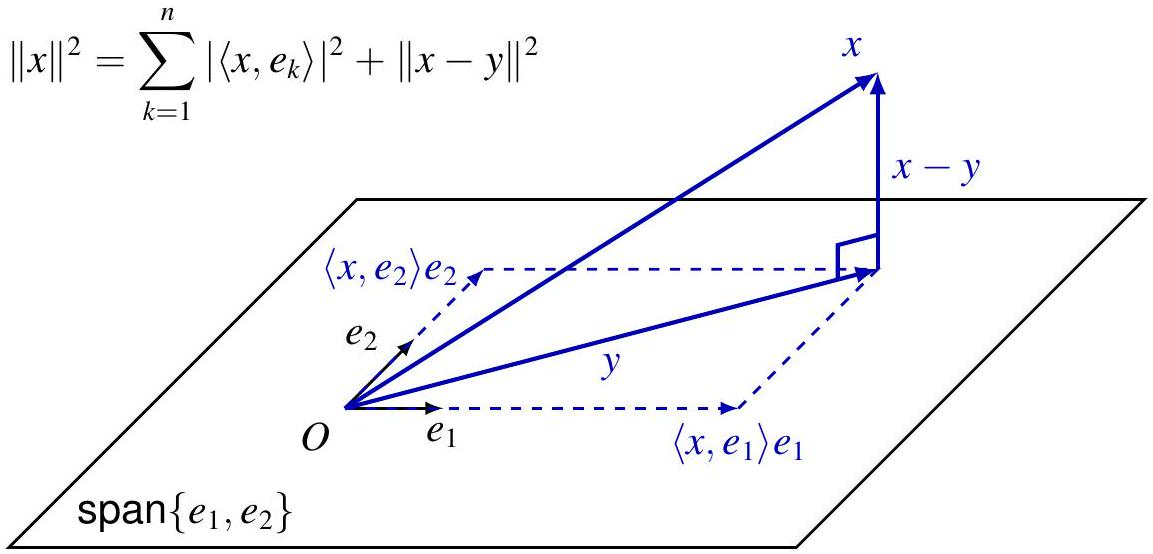
\includegraphics[width=0.8\linewidth,height=\textheight,keepaspectratio]{imglink/4cb8e742-a9ce-42fa-a004-42de4559e768-04.png}

思考：当\(n->\infty\)?
\end{block}
\end{frame}

\begin{frame}{帕塞瓦尔恒等式（帕塞瓦尔公式）}
\protect\phantomsection\label{ux5e15ux585eux74e6ux5c14ux6052ux7b49ux5f0fux5e15ux585eux74e6ux5c14ux516cux5f0f-2}
\begin{block}{完备正交规范序列}
\protect\phantomsection\label{ux5b8cux5907ux6b63ux4ea4ux89c4ux8303ux5e8fux5217}
在 Hilbert 空间 \(H\) 中，如果每一个元素 \(x \in H\)
都可以进行如下展开，则称标准正交序列 \(\{e_k : k \in \mathbb{N}\}\)
是\textbf{完备的} (Complete)：

\[x = \sum_{k=1}^{\infty} \langle x, e_k \rangle e_k\]

这意味着该序列的部分和在范数意义下收敛于 \(x\)，即：

\[\lim_{n \to \infty} \left\| x - \sum_{k=1}^{n} \langle x, e_k \rangle e_k \right\| = 0\]

\begin{itemize}
\tightlist
\item
  \textbf{标准正交基 (Orthonormal
  Basis)}：一个完备的标准正交序列也被称为该 Hilbert 空间 \(H\)
  的标准正交基。
\item
  \textbf{系数定义}：展开式中的系数 \(\langle x, e_k \rangle\) 称为
  \(x\) 关于基 \(\{e_k\}\) 的傅里叶系数或坐标。
\end{itemize}

经典示例

\begin{itemize}
\tightlist
\item
  \textbf{单位脉冲基}：\(\{\delta_k : k \in \mathbb{Z}\}\)
  是平方可和序列空间 \(\ell_2\) 的标准正交基。

  \begin{itemize}
  \tightlist
  \item
    其中 \(\delta_k[m] = 1\) (当 \(m=k\) 时) 且 \(\delta_k[m] = 0\) (当
    \(m \neq k\) 时)
  \end{itemize}
\end{itemize}
\end{block}
\end{frame}

\begin{frame}{傅里叶级数的均方收敛}
\protect\phantomsection\label{ux5085ux91ccux53f6ux7ea7ux6570ux7684ux5747ux65b9ux6536ux655b}
\begin{block}{定理}
\protect\phantomsection\label{ux5b9aux7406}
集合 \(\{e^{j k \frac{2\pi}{T} t} : k \in \mathbb{Z}\}\) 是 \(L_2(T)\)
空间的标准正交基。对于任何
\(x \in L_2(T)\)，其傅里叶级数在\textbf{均方意义}下收敛，即在 \(L_2\)
范数下满足：

\[\lim_{N \to \infty} \|x - S_N(x)\| = 0\]
\end{block}

\begin{block}{Parseval 公式 (帕塞瓦尔恒等式)}
\protect\phantomsection\label{parseval-ux516cux5f0f-ux5e15ux585eux74e6ux5c14ux6052ux7b49ux5f0f}
\[\sum_{k=-\infty}^{\infty} |\hat{x}[k]|^2 = \|x\|^2 = \frac{1}{T} \int_{T} |x(t)|^2 dt\]
\end{block}

\begin{block}{物理阐释：能量守恒 (Energy Conservation)}
\protect\phantomsection\label{ux7269ux7406ux9610ux91caux80fdux91cfux5b88ux6052-energy-conservation}
\begin{itemize}
\tightlist
\item
  \textbf{\(|\hat{x}[k]|^2\)}：第 \(k\) 次谐波分量的\textbf{平均功率}。
\item
  \textbf{\(\|x\|^2\)}：信号 \(x\) 的\textbf{总平均功率}。
\end{itemize}
\end{block}

\begin{block}{核心解读}
\protect\phantomsection\label{ux6838ux5fc3ux89e3ux8bfb}
\begin{enumerate}
\item
  \textbf{均方收敛 vs 逐点收敛}：
  这是一个非常重要的警示。即使傅里叶级数捕获了信号的所有``能量''（均方收敛），但在信号的跳变点（不连续点）附近，它可能仍然无法完全匹配信号的具体数值（即著名的
  \textbf{Gibbs 现象}）。
\item
  \textbf{频谱的本质}： Parseval
  等式建立了时域和频域之间的桥梁。它告诉我们，计算信号的功率既可以在时域（对平方求积分），也可以在频域（对系数平方求和）。在工程上，这意味着能量在变换过程中既没有丢失也没有凭空产生。
\item
  \textbf{正交性的威力}：
  之所以能写成这种简单的平方和形式，完全归功于复指数函数
  \(\{e^{j k \omega_0 t}\}\) 之间的相互\textbf{正交性}。
\end{enumerate}
\end{block}
\end{frame}

\begin{frame}{狄利克雷判别法}
\protect\phantomsection\label{ux72c4ux5229ux514bux96f7ux5224ux522bux6cd5}
\textbf{定理}：如果 \(x\) 满足以下 \textbf{狄利克雷条件 (Dirichlet
conditions)}：

\begin{enumerate}
\tightlist
\item
  \(x\) 是有界的，即 \(\|x\|_\infty < \infty\)；
\item
  \(x\) 是分段单调的，即存在周期的有限划分，使得 \(x\)
  在每个区间段上都是单调的；
\end{enumerate}

那么：

\[\lim_{N \to \infty} S_N(x)(t) = \frac{x(t_+) + x(t_-)}{2}\]

\textbf{示例：}

\[\lim_{N \to \infty} S_N(x)(t) = \begin{cases} 1, & t \in (n, n + \frac{1}{2}), \\ -1, & t \in (n - \frac{1}{2}, n), \\ 0, & t = \frac{n}{2}, \end{cases} \quad n \in \mathbb{Z}\]
\end{frame}

\begin{frame}{目录}
\protect\phantomsection\label{toc3}
\begin{itemize}
\tightlist
\item
  \hyperlink{sec31}{1. 线性时不变系统对复指数信号的响应}
\item
  \hyperlink{sec32}{2. 连续时间周期信号的傅里叶级数表示}
\item
  \hyperlink{sec33}{3. 连续时间傅里叶级数的收敛}
\item
  \hyperlink{sec34}{\textbf{4. 连续时间傅里叶级数的性质}}
\item
  \hyperlink{35}{5. 离散时间周期信号的傅里叶级数表示}
\item
  \hyperlink{sec36}{6. 离散时间傅里叶级数的性质}
\item
  \hyperlink{sec37}{7. 傅里叶级数与线性时不变系统}
\item
  \hyperlink{sec38}{8. 滤波}

  \begin{itemize}
  \tightlist
  \item
    \hyperlink{sec381}{频率成形滤波器}
  \item
    \hyperlink{sec382}{频率选择性滤波器}
  \item
    \hyperlink{sec383}{用微分方程描述的连续时间滤波器}
  \item
    \hyperlink{sec383}{用差分方程描述的离散时间滤波器}
  \end{itemize}
\end{itemize}
\end{frame}

\section{4. 连续时间傅里叶级数的性质}\label{sec34}

\begin{frame}{CT 傅里叶级数的性质}
\protect\phantomsection\label{ct-ux5085ux91ccux53f6ux7ea7ux6570ux7684ux6027ux8d28}
傅里叶级数建立了周期函数与双无限序列之间的对应关系：

\[
x \stackrel{\mathcal{F S}}{\longleftrightarrow} \hat{x} \quad \text { 或 } \quad x(t) \stackrel{\mathcal{F S}}{\longleftrightarrow} \hat{x}[k]
\]

\textbf{线性 (Linearity)} 如果 \(x, y\) 具有相同的周期
\(T\)，那么它们的线性组合 \(a x+b y\) 也是，并且：

\[
\widehat{a x+b y}=a \hat{x}+b \hat{y}
\]

证明：

\[
\begin{aligned}
(\widehat{a x+b y})[k] & =\left\langle a x+b y, e^{j k \omega_{0} t}\right\rangle \\
& =a\left\langle x, e^{j k \omega_{0} t}\right\rangle+b\left\langle y, e^{j k \omega_{0} t}\right\rangle \\
& =a \hat{x}[k]+b \hat{y}[k]
\end{aligned}
\]
\end{frame}

\begin{frame}{CT 傅里叶级数的性质}
\protect\phantomsection\label{ct-ux5085ux91ccux53f6ux7ea7ux6570ux7684ux6027ux8d28-1}
\textbf{时移 (Time shifting)} 如果 \(x\) 周期为 \(T\) 且
\(\omega_{0}=\frac{2 \pi}{T}\)，

\[
\widehat{\tau_{t_{0}} x}=E_{-\omega_{0} t_{0}} \hat{x} \quad \text { 或 } \quad x\left(t-t_{0}\right) \stackrel{\mathcal{F S}}{\longleftrightarrow} e^{-j k \omega_{0} t_{0}} \hat{x}[k]
\]

其中 \(\left(E_{a} \hat{x}\right)[k]=e^{j a k} \hat{x}[k]\) \textbf{时移
⟺ 频率上的线性相位变化}

证明：

\[
\begin{aligned}
\left(\widehat{\tau_{t_{0}}} x\right)[k] & =\left\langle\tau_{t_{0}} x, e^{j k \omega_{0} t}\right\rangle=\left\langle x, \tau_{-t_{0}} e^{j k \omega_{0} t}\right\rangle \\
& =\left\langle x, e^{j k \omega_{0}\left(t+t_{0}\right)}\right\rangle=\left\langle x, e^{j k \omega_{0} t_{0}} e^{j k \omega_{0} t}\right\rangle \\
& =e^{-j k \omega_{0} t_{0}}\left\langle x, e^{j k \omega_{0} t}\right\rangle=e^{-j k \omega_{0} t_{0}} \hat{x}[k]=\left(E_{-\omega_{0} t_{0}} \hat{x}\right)[k]
\end{aligned}
\]

例子：\(\cos (t)=\frac{1}{2} e^{j t}+\frac{1}{2} e^{-j t}, \sin (t)=\cos \left(t-\frac{\pi}{2}\right)=\frac{-j}{2} e^{j t}+\frac{j}{2} e^{-j t}\)

\hyperlink{toc4}{返回目录}
\end{frame}

\begin{frame}{傅里叶级数 (回顾)}
\protect\phantomsection\label{ux5085ux91ccux53f6ux7ea7ux6570-ux56deux987e}
周期为 \(T\) 且 \(\omega_{0}=\frac{2 \pi}{T}\) 的信号 \(x\)
的傅里叶级数：

\[
x(t)=\sum_{k=-\infty}^{\infty} \hat{x}[k] e^{j k \omega_{0} t}
\]

周期函数与双无限序列之间的对应关系；时域 vs.~频域：

\[
x \stackrel{\mathcal{F S}}{\longleftrightarrow} \hat{x} \quad \text { 或 } \quad x(t) \stackrel{\mathcal{F S}}{\longleftrightarrow} \hat{x}[k]
\]

\begin{itemize}
\tightlist
\item
  \(\hat{x}\) 由 \(x\) 在``基'' \(\left\{e^{j k \omega_{0} t}\right\}\)
  下的展开系数组成
\item
  仅凭 \(\hat{x}\) 不能唯一确定 \(x\)，
\item
  还需要知道基函数，或者等价地，知道周期 \(T\) 或基频 \(\omega_{0}\)
\item
  相同的系数配合不同的基（周期）会给出不同的函数（稍后详述）
\end{itemize}
\end{frame}

\begin{frame}{线性 (Linearity)}
\protect\phantomsection\label{ux7ebfux6027-linearity}
如果 \(x, y\) 具有相同的周期 \(T\)，那么它们的线性组合 \(a x+b y\)
也是，并且：

\[
\widehat{a x+b y}=a \hat{x}+b \hat{y}
\]

证明：

\[
\begin{aligned}
(\widehat{a x+b y})[k] & =\left\langle a x+b y, e^{j k \omega_{0} t}\right\rangle \\
& =a\left\langle x, e^{j k \omega_{0} t}\right\rangle+b\left\langle y, e^{j k \omega_{0} t}\right\rangle \\
& =a \hat{x}[k]+b \hat{y}[k]
\end{aligned}
\]

另一种证明思路：

\[
\left.\begin{array}{l}
x(t)=\sum_{k} \hat{x}[k] e^{j k \omega_{0} t} \\
y(t)=\sum_{k} \hat{y}[k] e^{j k \omega_{0} t}
\end{array}\right\} \Longrightarrow a x(t)+b y(t)=\sum_{k}(a \hat{x}[k]+b \hat{y}[k]) e^{j k \omega_{0} t}
\]
\end{frame}

\begin{frame}{时移 (Time Shifting)}
\protect\phantomsection\label{ux65f6ux79fb-time-shifting}
如果 \(x\) 周期为 \(T\) 且 \(\omega_{0}=\frac{2 \pi}{T}\)，

\[
\widehat{\tau_{t_{0}} x}=E_{-\omega_{0} t_{0}} \hat{x} \quad \text { 或 } \quad x\left(t-t_{0}\right) \stackrel{\mathcal{F S}}{\longleftrightarrow} e^{-j k \omega_{0} t_{0}} \hat{x}[k]
\]

其中 \(\left(E_{a} \hat{x}\right)[k]=e^{j a k} \hat{x}[k]\)

\textbf{时移 ⟺ 频率上的线性相位变化}

证明：

\[
\begin{aligned}
\left(\widehat{\tau_{t_{0}}} x\right)[k] & =\left\langle\tau_{t_{0}} x, e^{j k \omega_{0} t}\right\rangle=\left\langle x, \tau_{-t_{0}} e^{j k \omega_{0} t}\right\rangle \\
& =\left\langle x, e^{j k \omega_{0}\left(t+t_{0}\right)}\right\rangle=\left\langle x, e^{j k \omega_{0} t_{0}} e^{j k \omega_{0} t}\right\rangle \\
& =e^{-j k \omega_{0} t_{0}}\left\langle x, e^{j k \omega_{0} t}\right\rangle=e^{-j k \omega_{0} t_{0}} \hat{x}[k]=\left(E_{-\omega_{0} t_{0}} \hat{x}\right)[k]
\end{aligned}
\]

例子：\(\cos (t)=\frac{1}{2} e^{j t}+\frac{1}{2} e^{-j t}, \sin (t)=\cos \left(t-\frac{\pi}{2}\right)=\frac{-j}{2} e^{j t}+\frac{j}{2} e^{-j t}\)
\end{frame}

\begin{frame}{频移 (Frequency Shifting)}
\protect\phantomsection\label{ux9891ux79fb-frequency-shifting}
如果 \(x\) 周期为 \(T\) 且 \(\omega_{0}=\frac{2 \pi}{T}\)，

\[
\widehat{E_{m \omega_{0}} x}=\tau_{m} \hat{x} \quad \text { 或 } \quad e^{j m \omega_{0} t} x(t) \stackrel{\mathcal{F S}}{\longleftrightarrow} \hat{x}[k-m]
\]

其中 \(\left(E_{a} x\right)(t)=e^{j a t} x(t)\)

\textbf{谐波指数调制 ⟹ 频移}

证明：

\[
\begin{aligned}
\left(\widehat{E_{m \omega_{0}}} x\right)[k] & =\left\langle E_{m \omega_{0}} x, e^{j k \omega_{0} t}\right\rangle=\left\langle x, E_{-m \omega_{0}} e^{j k \omega_{0} t}\right\rangle \\
& =\left\langle x, e^{j(k-m) \omega_{0} t}\right\rangle=\hat{x}[k-m]
\end{aligned}
\]

注意：用非谐波指数信号进行调制可能会改变基频，甚至导致非周期信号。
\end{frame}

\begin{frame}{频移示例}
\protect\phantomsection\label{ux9891ux79fbux793aux4f8b}
例子：\(x(t)=1+\cos \left(\omega_{0} t\right)=1+\frac{1}{2} e^{j \omega_{0} t}+\frac{1}{2} e^{-j \omega_{0} t}\)

\[
y(t)=e^{j 3 \omega_{0} t} x(t)=e^{j 3 \omega_{0} t}+\frac{1}{2} e^{j 4 \omega_{0} t}+\frac{1}{2} e^{j 2 \omega_{0} t}
\]

\begin{columns}[T]
\begin{column}{0.5\linewidth}
\pandocbounded{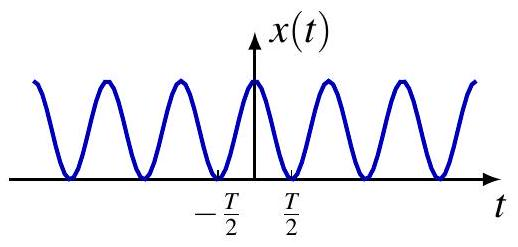
\includegraphics[keepaspectratio]{imglink/9070b8cb-a2bd-4c7b-959f-e6b33147f2c9-07_3.png}}

\pandocbounded{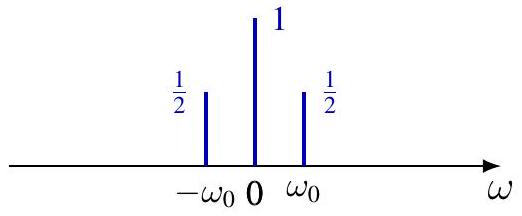
\includegraphics[keepaspectratio]{imglink/9070b8cb-a2bd-4c7b-959f-e6b33147f2c9-07.png}}
\end{column}

\begin{column}{0.5\linewidth}
\pandocbounded{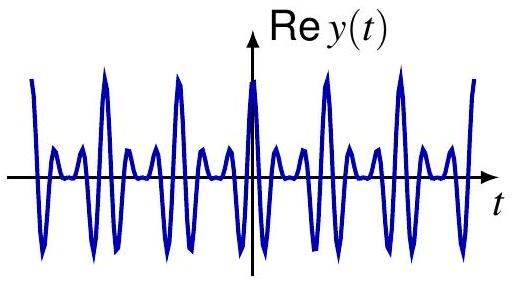
\includegraphics[keepaspectratio]{imglink/9070b8cb-a2bd-4c7b-959f-e6b33147f2c9-07_4.png}}

\pandocbounded{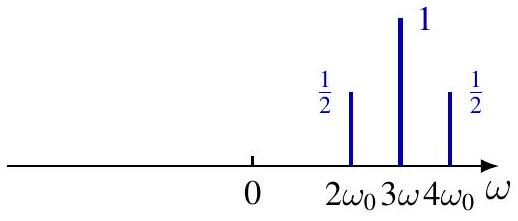
\includegraphics[keepaspectratio]{imglink/9070b8cb-a2bd-4c7b-959f-e6b33147f2c9-07_2.png}}
\end{column}
\end{columns}
\end{frame}

\begin{frame}{频移示例}
\protect\phantomsection\label{ux9891ux79fbux793aux4f8b-1}
例子：\(x(t)=1+\cos \left(\omega_{0} t\right)=1+\frac{1}{2} e^{j \omega_{0} t}+\frac{1}{2} e^{-j \omega_{0} t}\)

\[
\begin{aligned}
z(t)=\cos \left(3 \omega_{0} t\right) x(t)=\operatorname{Re} y(t) & =\frac{1}{2} e^{j 3 \omega_{0} t}+\frac{1}{4} e^{j 4 \omega_{0} t}+\frac{1}{4} e^{j 2 \omega_{0} t} \\
& +\frac{1}{2} e^{-j 3 \omega_{0} t}+\frac{1}{4} e^{-j 4 \omega_{0} t}+\frac{1}{4} e^{-j 2 \omega_{0} t}
\end{aligned}
\]

\begin{columns}[T]
\begin{column}{0.5\linewidth}
\pandocbounded{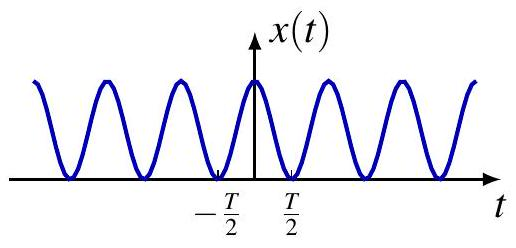
\includegraphics[keepaspectratio]{imglink/9070b8cb-a2bd-4c7b-959f-e6b33147f2c9-08_3.png}}

\pandocbounded{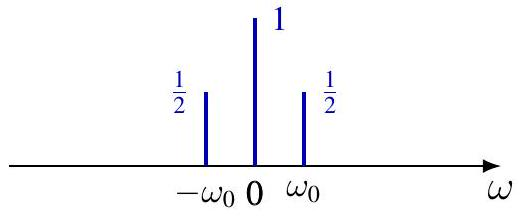
\includegraphics[keepaspectratio]{imglink/9070b8cb-a2bd-4c7b-959f-e6b33147f2c9-08_2.png}}
\end{column}

\begin{column}{0.5\linewidth}
\pandocbounded{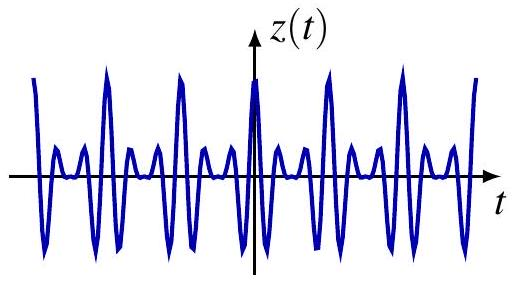
\includegraphics[keepaspectratio]{imglink/9070b8cb-a2bd-4c7b-959f-e6b33147f2c9-08_4.png}}

\pandocbounded{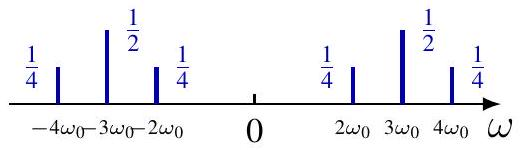
\includegraphics[keepaspectratio]{imglink/9070b8cb-a2bd-4c7b-959f-e6b33147f2c9-08.png}}
\end{column}
\end{columns}
\end{frame}

\begin{frame}{时间反转 (Time Reversal)}
\protect\phantomsection\label{ux65f6ux95f4ux53cdux8f6c-time-reversal}
如果 \(x\) 周期为 \(T\)，

\[
\widehat{R x}=R \hat{x} \quad \text { 或 } \quad x(-t) \stackrel{\mathcal{F S}}{\longleftrightarrow} \hat{x}[-k]
\]

时间反转与傅里叶级数可交换

\begin{center}
\pandocbounded{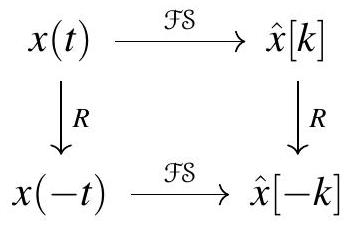
\includegraphics[keepaspectratio]{imglink/9070b8cb-a2bd-4c7b-959f-e6b33147f2c9-09.png}}
\end{center}

证明：

\[
(\widehat{R x})[k]=\left\langle R x, e^{j k \omega_{0} t}\right\rangle=\left\langle x, R e^{j k \omega_{0} t}\right\rangle=\left\langle x, e^{-j k \omega_{0} t}\right\rangle=\hat{x}[-k]
\]

推论：傅里叶级数保持奇/偶对称性，即 \(x\) 偶
\(\Longleftrightarrow \hat{x}\) 偶，\(\quad x\) 奇
\(\Longleftrightarrow \hat{x}\) 奇
\end{frame}

\begin{frame}{时间缩放 (Time Scaling)}
\protect\phantomsection\label{ux65f6ux95f4ux7f29ux653e-time-scaling}
如果 \(x\) 周期为 \(T\)，那么 \(S_{a} x\) 周期为 \(T / a\)

\[
\widehat{S_{a} x}=\hat{x} \quad \text { 或 } \quad x(a t) \stackrel{\mathcal{F S}}{\longleftrightarrow} \hat{x}[k]
\]

时间缩放保持傅里叶系数不变，但改变基频

\begin{columns}[T]
\begin{column}{0.4\linewidth}
\begin{aligned}
x(t) & =\sum_{k=-\infty}^{\infty} \hat{x}[k] e^{j k \omega_{0} t} \\
x(a t) & =\sum_{k=-\infty}^{\infty} \hat{x}[k] e^{j k\left(a \omega_{0}\right) t}
\end{aligned}
\end{column}

\begin{column}{0.3\linewidth}
\pandocbounded{
\includegraphics[keepaspectratio]{imglink/timescaling.png}}\hfill
\end{column}

\begin{column}{0.3\linewidth}
\end{column}
\end{columns}
\end{frame}

\begin{frame}{时间缩放}
\protect\phantomsection\label{ux65f6ux95f4ux7f29ux653e}
\[
x(t)=\sum_{k=-\infty}^{\infty} \hat{x}[k] e^{j k \omega_{0} t}
\]

对比
\(\quad x(a t)=\sum_{k=-\infty}^{\infty} \hat{x}[k] e^{j k\left(a \omega_{0}\right) t}\)

\begin{columns}[T]
\begin{column}{0.5\linewidth}
\pandocbounded{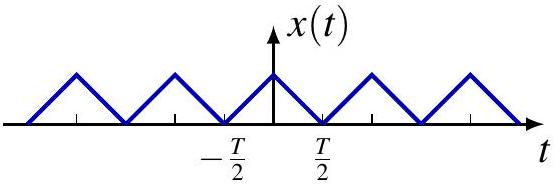
\includegraphics[keepaspectratio]{imglink/9070b8cb-a2bd-4c7b-959f-e6b33147f2c9-11.png}}

\pandocbounded{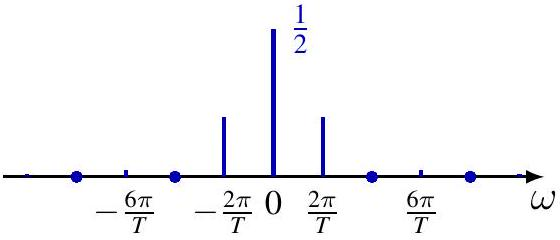
\includegraphics[keepaspectratio]{imglink/9070b8cb-a2bd-4c7b-959f-e6b33147f2c9-11_4.png}}
\end{column}

\begin{column}{0.5\linewidth}
\pandocbounded{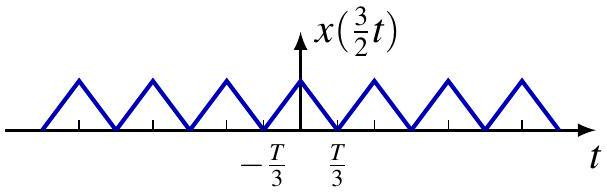
\includegraphics[keepaspectratio]{imglink/9070b8cb-a2bd-4c7b-959f-e6b33147f2c9-11_2.png}}

\pandocbounded{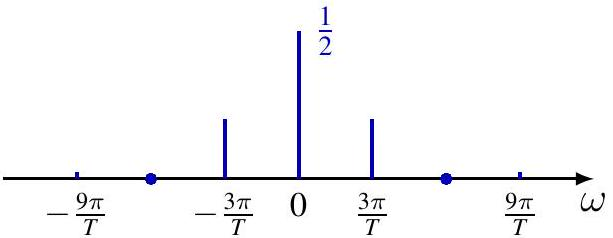
\includegraphics[keepaspectratio]{imglink/9070b8cb-a2bd-4c7b-959f-e6b33147f2c9-11_3.png}}
\end{column}
\end{columns}

时域压缩 ⟺ 频域（基频）扩展

时域扩展 ⟹ 频域（基频）压缩
\end{frame}

\begin{frame}{微分 (Differentiation)}
\protect\phantomsection\label{ux5faeux5206-differentiation}
如果 \(x\) 周期为 \(T\)，那么其导数 \(x^{\prime}\) 也是，且

\[
\widehat{x^{\prime}}=M_{\omega_{0}} \hat{x} \quad \text { 或 } \quad x^{\prime}(t) \stackrel{\mathcal{F S}}{\longleftrightarrow} j k \omega_{0} \hat{x}[k]
\]

其中 \(\left(M_{a} \hat{x}\right)[k]=j a k \hat{x}[k]\) \textbf{时域微分
⟹ 频域乘以 \(j k \omega_{0}\)}

证明：

\[
\begin{aligned}
\widehat{x^{\prime}}[k] & =\frac{1}{T} \int_{T} x^{\prime}(t) e^{-j k \omega_{0} t} d t \\
& =\left.\frac{1}{T}\left[x(t) e^{-j k \omega_{0} t}\right]\right|_{0} ^{T}+j k \omega_{0}\left(\frac{1}{T} \int_{T} x(t) e^{-j k \omega_{0} t} d t\right)=j k \omega_{0} \hat{x}[k]
\end{aligned}
\]

或者，逐项求导：

\[
x(t)=\sum_{k} \hat{x}[k] e^{j k \omega_{0} t} \Longrightarrow x^{\prime}(t)=\sum_{k} j k \omega_{0} \hat{x}[k] e^{-j k \omega_{0} t}
\]
\end{frame}

\begin{frame}{积分 (Integration)}
\protect\phantomsection\label{ux79efux5206-integration}
如果 \(x\) 周期为 \(T\) 且有傅里叶级数

\[
x(t)=\sum_{k=-\infty}^{\infty} \hat{x}[k] e^{j k \omega_{0} t}
\]

逐项积分：

\[
\begin{aligned}
y(t) \triangleq \int_{0}^{t} x(s) d s & =\hat{x}[0] t+\sum_{k \neq 0} \hat{x}[k] \frac{e^{j k \omega_{0} t}-1}{j k \omega_{0}} \\
& =\hat{x}[0] t-\sum_{k \neq 0} \frac{\hat{x}[k]}{j k \omega_{0}}+\sum_{k \neq 0} \frac{1}{j k \omega_{0}} \hat{x}[k] e^{j k \omega_{0} t}
\end{aligned}
\]

\begin{itemize}
\item
  \(y\) 是周期的，当且仅当 \(\hat{x}[0]=0\)，即 \(x\) 没有直流分量
\item
  如果 \(\hat{x}[0]=0, y\) 周期为 \(T\)，
  \(\hat{y}[k]=\frac{1}{j k \omega_{0}} \hat{x}[k] \quad \text { 对于 } k \neq 0\)
\item
  \textbf{\(\sum_{k \neq 0} \frac{\hat{x}[k]}{j k \omega_{0}}+\sum_{k \neq 0}\)
  去哪里了?}
\end{itemize}

直流分量
\end{frame}

\begin{frame}{例子：三角波}
\protect\phantomsection\label{ux4f8bux5b50ux4e09ux89d2ux6ce2}
\pandocbounded{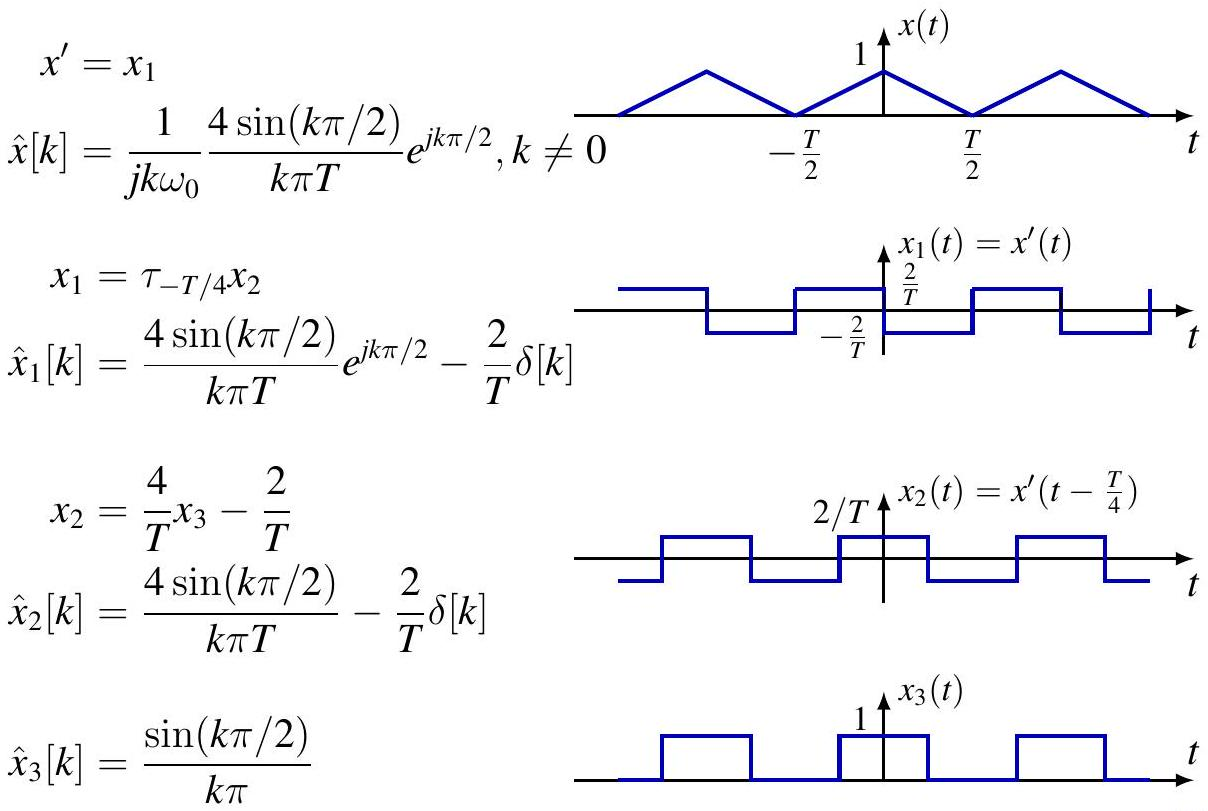
\includegraphics[keepaspectratio]{imglink/9070b8cb-a2bd-4c7b-959f-e6b33147f2c9-14.png}}
\end{frame}

\begin{frame}{乘法 (Multiplication)}
\protect\phantomsection\label{ux4e58ux6cd5-multiplication}
如果 \(x\) 和 \(y\) 具有相同的周期 \(T\)，那么它们的乘积 \(x y\)
也是，且

\[
\begin{gathered}
\widehat{x y}=\hat{x} * \hat{y} \quad \text { 或 } \quad x(t) y(t) \stackrel{\mathcal{F S}}{\longleftrightarrow} \sum_{m=-\infty}^{\infty} \hat{x}[m] \hat{y}[k-m] \\
\text { 时域乘法 } \Longleftrightarrow \text { 频域卷积 }
\end{gathered}
\]

证明：

\[
\begin{aligned}
x(t) y(t) & =\left(\sum_{m=-\infty}^{\infty} \hat{x}[m] e^{j m \omega_{0} t}\right)\left(\sum_{\ell=-\infty}^{\infty} \hat{y}[\ell] e^{j \ell \omega_{0} t}\right) \\
& =\sum_{m=-\infty}^{\infty} \sum_{\ell=-\infty}^{\infty} \hat{x}[m] \hat{y}[\ell] e^{j(m+\ell) \omega_{0} t} \\
& =\sum_{k=-\infty}^{\infty}\left(\sum_{m=-\infty}^{\infty} \hat{x}[m] \hat{y}[k-m]\right) e^{j k \omega_{0} t} \quad(k=m+\ell)
\end{aligned}
\]
\end{frame}

\begin{frame}{周期卷积 (Periodic Convolution)}
\protect\phantomsection\label{ux5468ux671fux5377ux79ef-periodic-convolution}
具有相同周期 \(T\) 的 \(x\) 和 \(y\) 的周期卷积 \(x * y\) 定义为：

\[
(x * y)(t)=\int_{T} x(\tau) y(t-\tau) d \tau
\]

性质：

\begin{itemize}
\tightlist
\item
  交换律
\end{itemize}

\[
x * y=y * x
\]

\begin{itemize}
\tightlist
\item
  结合律
\end{itemize}

\[
(x * y) * z=x *(y * z)
\]

\begin{itemize}
\tightlist
\item
  双线性
\end{itemize}

\[
\left(\sum_{i} a_{i} x_{i}\right) *\left(\sum_{j} b_{j} y_{j}\right)=\sum_{i, j} a_{i} b_{j}\left(x_{i} * y_{j}\right)
\]
\end{frame}

\begin{frame}{周期卷积性质}
\protect\phantomsection\label{ux5468ux671fux5377ux79efux6027ux8d28}
傅里叶系数满足

\[
\widehat{x * y}=T \hat{x} \hat{y} \quad \text { 或 } \quad(x * y)(t) \stackrel{\mathcal{F S}}{\longleftrightarrow} T \hat{x}[k] \hat{y}[k]
\]

\textbf{时域卷积 ⟹ 频域乘法}

证明：

\[
\begin{aligned}
(\widehat{x * y})[k] & =\frac{1}{T} \int_{T}(x * y)(t) e^{-j k \omega_{0} t} d t \\
& =\frac{1}{T} \int_{T}\left(\int_{T} x(\tau) y(t-\tau) d \tau\right) e^{-j k \omega_{0} t} d t \\
& =\int_{T} x(\tau)\left(\frac{1}{T} \int_{T} y(t-\tau) e^{-j k \omega_{0} t} d t\right) d \tau \\
& =\int_{T} x(\tau)\left(e^{-j k \omega_{0} \tau} \hat{y}[k]\right) d \tau=T \hat{x}[k] \hat{y}[k]
\end{aligned}
\]
\end{frame}

\begin{frame}{共轭与对称 (Conjugation and Symmetry)}
\protect\phantomsection\label{ux5171ux8f6dux4e0eux5bf9ux79f0-conjugation-and-symmetry}
如果 \(x\) 周期为 \(T\)，那么其复共轭 \(\bar{x}=x^{*}\) 也是，且

\[
\widehat{x^{*}}=R \hat{x}^{*} \quad \text { 或 } \quad x^{*}(t) \stackrel{\mathcal{F S}}{\longleftrightarrow}(\hat{x}[-k])^{*}
\]

证明：

\[
\widehat{x^{*}}[k]=\left\langle x^{*}, e^{j k \omega_{0} t}\right\rangle=\overline{\left\langle x, e^{-j k \omega_{0} t}\right\rangle}=\overline{\hat{x}[-k]}
\]

推论：如果 \(x\) 是实信号，则 \(\hat{x}\) 是共轭对称的，即

\[
\hat{x}[-k]=\overline{\hat{x}[k]}
\]

推论：如果 \(x\) 是实偶信号，则 \(\hat{x}\) 也是实偶信号

\[
\hat{x}[k]=\hat{x}[-k]=\overline{\hat{x}[k]}
\]

推论：如果 \(x\) 是实奇信号，则 \(\hat{x}\) 是纯虚奇信号

\[
-\hat{x}[k]=\hat{x}[-k]=\overline{\hat{x}[k]}
\]
\end{frame}

\begin{frame}{周期冲激列}
\protect\phantomsection\label{ux5468ux671fux51b2ux6fc0ux5217}
\[
x(t)=\sum_{k=-\infty}^{\infty} \delta(t-k T)
\]

\pandocbounded{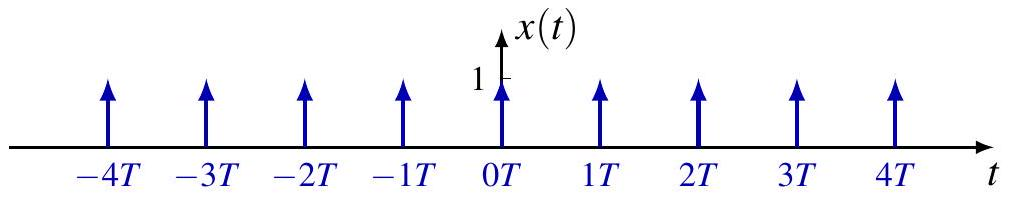
\includegraphics[keepaspectratio]{imglink/4cb8e742-a9ce-42fa-a004-42de4559e768-23.png}}

对于``足够好''的函数，例如\(\phi\),具有紧支撑的无限可微函数：

\[
\begin{gathered}
(\phi * x)(t)=\sum_{k=-\infty}^{\infty} \phi(t-k T) \\
\int_{\mathbb{R}} \phi(t) x(t) d t=\sum_{k=-\infty}^{\infty} \int_{\mathbb{R}} \phi(t) \delta(t-k T) d t=\sum_{k=-\infty}^{\infty} \phi(k T)
\end{gathered}
\]
\end{frame}

\begin{frame}{周期冲激列}
\protect\phantomsection\label{ux5468ux671fux51b2ux6fc0ux5217-1}
\[
x(t)=\sum_{k=-\infty}^{\infty} \delta(t-k T)
\]

\begin{center}
\pandocbounded{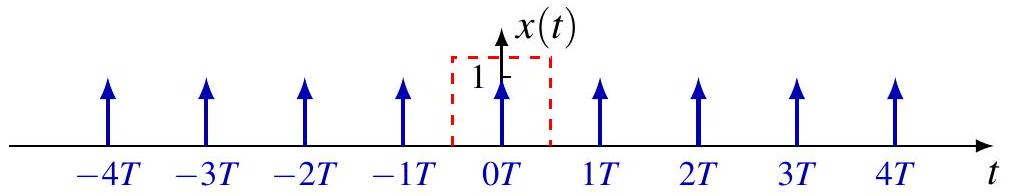
\includegraphics[keepaspectratio]{imglink/4cb8e742-a9ce-42fa-a004-42de4559e768-24.png}}
\end{center}

傅里叶系数：

\[
\hat{x}[k]=\frac{1}{T} \int_{-T / 2}^{T / 2} \delta(t) e^{-j k \frac{2 \pi}{T} t} d t=\frac{1}{T}
\]

傅里叶级数：

\[
x(t)=\sum_{k=-\infty}^{\infty} \frac{1}{T} e^{j k \frac{2 \pi}{T} t}=\lim _{N \rightarrow \infty} \frac{1}{T} D_{N}\left(\frac{2 \pi}{T} t\right)
\]

其中 \(D_{N}\) 是狄利克雷核。
\end{frame}

\begin{frame}{周期冲激列}
\protect\phantomsection\label{ux5468ux671fux51b2ux6fc0ux5217-2}
\[
x(t)=\sum_{k=-\infty}^{\infty} \delta(t-k T)=\sum_{k=-\infty}^{\infty} \frac{1}{T} e^{j k \frac{2 \pi}{T} t}
\]

\begin{center}
\pandocbounded{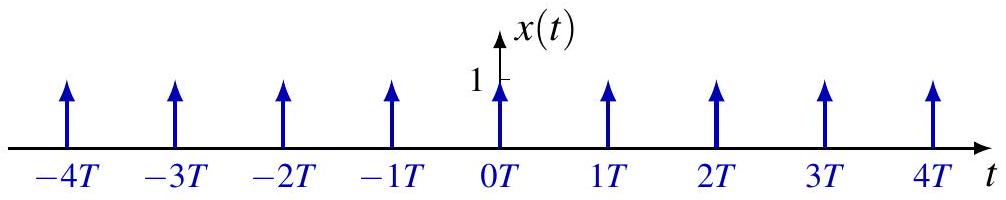
\includegraphics[keepaspectratio]{imglink/4cb8e742-a9ce-42fa-a004-42de4559e768-25_2.png}}
\end{center}

\begin{center}
\pandocbounded{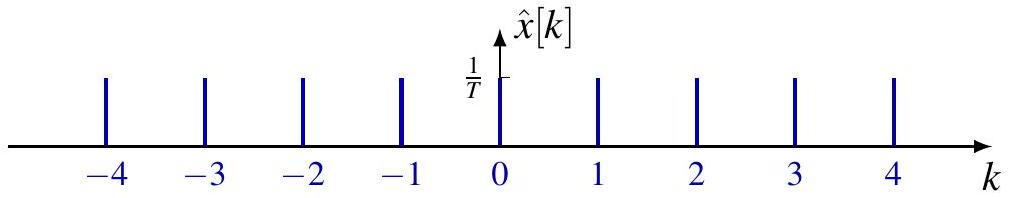
\includegraphics[keepaspectratio]{imglink/4cb8e742-a9ce-42fa-a004-42de4559e768-25.png}}
\end{center}
\end{frame}

\begin{frame}{周期冲激列}
\protect\phantomsection\label{ux5468ux671fux51b2ux6fc0ux5217-3}
\[
\begin{aligned}
\int_{\mathbb{R}} \phi(t) x(t) d t & =\lim _{N \rightarrow \infty} \frac{1}{T} \int_{\mathbb{R}} \phi(t) D_{N}\left(-\frac{2 \pi}{T} t\right) d t \quad\left(D_{N} \text { is even }\right) \\
& =\lim _{N \rightarrow \infty} \frac{1}{2 \pi} \int_{\mathbb{R}} \phi\left(-\frac{T}{2 \pi} t\right) D_{N}(t) d t \\
& =\lim _{N \rightarrow \infty} \sum_{k=-\infty}^{\infty} \frac{1}{2 \pi} \int_{(2 k-1) \pi}^{(2 k+1) \pi} \phi\left(-\frac{T}{2 \pi} t\right) D_{N}(t) d t \\
& =\sum_{k=-\infty}^{\infty} \lim _{N \rightarrow \infty} \frac{1}{2 \pi} \int_{-\pi}^{\pi} \phi\left(\frac{T}{2 \pi}(2 \pi k-t)\right) D_{N}(t-2 k \pi) d t \\
& \left.=\sum_{k=-\infty}^{\infty} \lim _{N \rightarrow \infty} \frac{1}{2 \pi} \int_{-\pi}^{\pi} \phi\left(\frac{T}{2 \pi}(2 \pi k-t)\right)_{\left(D_{N}\right.} \text { is } 2 \pi \text {-periodic }\right) \\
& =\sum_{k=-\infty}^{\infty} \lim _{N \rightarrow \infty} S_{N}(\phi)(k T)=\sum_{k=-\infty}^{\infty} \phi(k T)
\end{aligned}
\]
\end{frame}

\begin{frame}{与周期方波的关系}
\protect\phantomsection\label{ux4e0eux5468ux671fux65b9ux6ce2ux7684ux5173ux7cfb}
\begin{center}
\pandocbounded{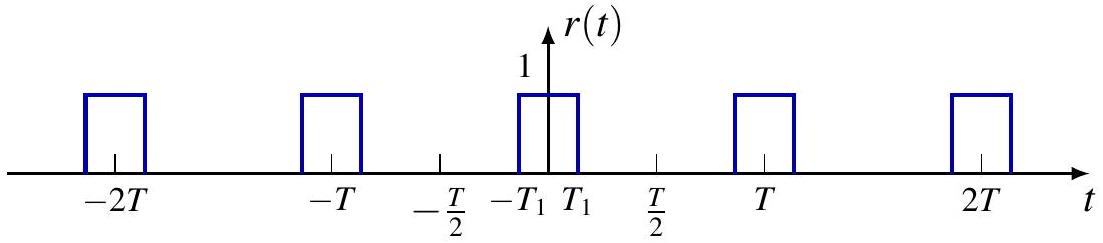
\includegraphics[keepaspectratio]{imglink/4cb8e742-a9ce-42fa-a004-42de4559e768-27_2.png}}
\end{center}

\begin{center}
\pandocbounded{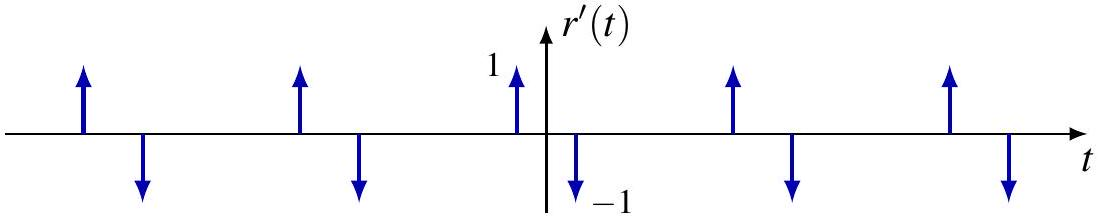
\includegraphics[keepaspectratio]{imglink/4cb8e742-a9ce-42fa-a004-42de4559e768-27.png}}
\end{center}

\[
\begin{aligned}
r^{\prime}(t) & =x\left(t+T_{1}\right)-x\left(t-T_{1}\right) \\
\widehat{r^{\prime}}[k] & =\left(e^{j k \omega_{0} T_{1}}-e^{-j k \omega_{0} T_{1}}\right) \hat{x}[k]=\frac{2 j \sin \left(k \omega_{0} T_{1}\right)}{T} \\
\hat{r}[k] & =\frac{1}{j k \omega_{0}} \widehat{r^{\prime}}[k]=\frac{\sin \left(k \omega_{0} T_{1}\right)}{k \pi}, \quad k \neq 0
\end{aligned}
\]
\end{frame}

\begin{frame}{目录}
\protect\phantomsection\label{toc4}
\begin{itemize}
\tightlist
\item
  \hyperlink{sec31}{1. 线性时不变系统对复指数信号的响应}
\item
  \hyperlink{sec32}{2. 连续时间周期信号的傅里叶级数表示}
\item
  \hyperlink{sec33}{3. 连续时间傅里叶级数的收敛}
\item
  \hyperlink{sec34}{4. 连续时间傅里叶级数的性质}
\item
  \hyperlink{35}{\textbf{5. 离散时间周期信号的傅里叶级数表示}}
\item
  \hyperlink{sec36}{6. 离散时间傅里叶级数的性质}
\item
  \hyperlink{sec37}{7. 傅里叶级数与线性时不变系统}
\item
  \hyperlink{sec38}{8. 滤波}

  \begin{itemize}
  \tightlist
  \item
    \hyperlink{sec381}{频率成形滤波器}
  \item
    \hyperlink{sec382}{频率选择性滤波器}
  \item
    \hyperlink{sec383}{用微分方程描述的连续时间滤波器}
  \item
    \hyperlink{sec383}{用差分方程描述的离散时间滤波器}
  \end{itemize}
\end{itemize}
\end{frame}

\section{5. 离散时间周期信号的傅里叶级数表示}\label{sec35}

\begin{frame}{DT 周期信号}
\protect\phantomsection\label{dt-ux5468ux671fux4fe1ux53f7}
回顾：DT 信号是周期的，周期为 \(N\)，如果

\[
x=\tau_{N} x \quad \text { 或 } \quad x[n]=x[n+N], \forall n \in \mathbb{Z}
\]

\begin{itemize}
\tightlist
\item
  基波周期 \(N\)：最小的正周期
\item
  基频
  \(\begin{cases}\frac{2 \pi}{N}, & \text { 如果 } N>1 \\ 0, & \text { 如果 } N=1\end{cases}\)
\end{itemize}

复指数信号
\(\phi_{N}^{k}[n]=e^{j k \frac{2 \pi}{N} n}=e^{j k \omega_{0} n}\)
是周期的，具有：

\begin{itemize}
\tightlist
\item
  周期 \(N\) 和基波周期 \(\frac{N}{\operatorname{gcd}(N, k)}\)
\item
  基频
  \(\omega_{k}= \begin{cases}0, & \text { 如果 } N \mid k \\ \omega_{0} \cdot \operatorname{gcd}(k, N), & \text { 其他 }\end{cases}\)，总是
  \(\omega_{0}=\frac{2 \pi}{N}\) 的整数倍
\end{itemize}
\end{frame}

\begin{frame}{DT 傅里叶基的有限性}
\protect\phantomsection\label{dt-ux5085ux91ccux53f6ux57faux7684ux6709ux9650ux6027}
傅里叶级数用谐波相关的复指数 \(\phi_{N}^{k}\) 表示 \(N\)-周期信号

\[
x=\sum_{k} c_{k} \phi_{N}^{k}, \quad \text { 或 } \quad x[n]=\sum_{k} c_{k} \phi_{N}^{k}[n]=\sum_{k} c_{k} e^{j k \frac{2 \pi}{N} n}
\]

与 CT 情况的关键区别：\(\phi_{N}^{k+r N}=\phi_{N}^{k}\)，所以只有 \(N\)
个不同的 \(\phi_{N}^{k}\)，傅里叶基是有限的，即

\[
\left\{\phi_{N}^{k}: k \in \mathbb{Z}\right\}=\left\{\phi_{N}^{k}: k \in[N]\right\}
\]

其中 \([N]=\{0,1, \ldots, N-1\}\)（可以理解为
\([N]=\{\overline{0}, \overline{1}, \ldots, \overline{N-1}\}\)）。

证明：对于 \(r \in \mathbb{Z}\)， \[
\phi_{N}^{k+r N}[n]=e^{j(k+r N) \frac{2 \pi}{N} n}=e^{j k \frac{2 \pi}{N} n} e^{j r 2 \pi n}=e^{j k \frac{2 \pi}{N} n}=\phi_{N}^{k}[n]
\]
\end{frame}

\begin{frame}{DT 傅里叶基的有限性 (图示)}
\protect\phantomsection\label{dt-ux5085ux91ccux53f6ux57faux7684ux6709ux9650ux6027-ux56feux793a}
\(\phi_{N}^{k}\) 示例， \(N=4\) 和 \(k=0,1, \ldots, 8\)

\begin{center}
\pandocbounded{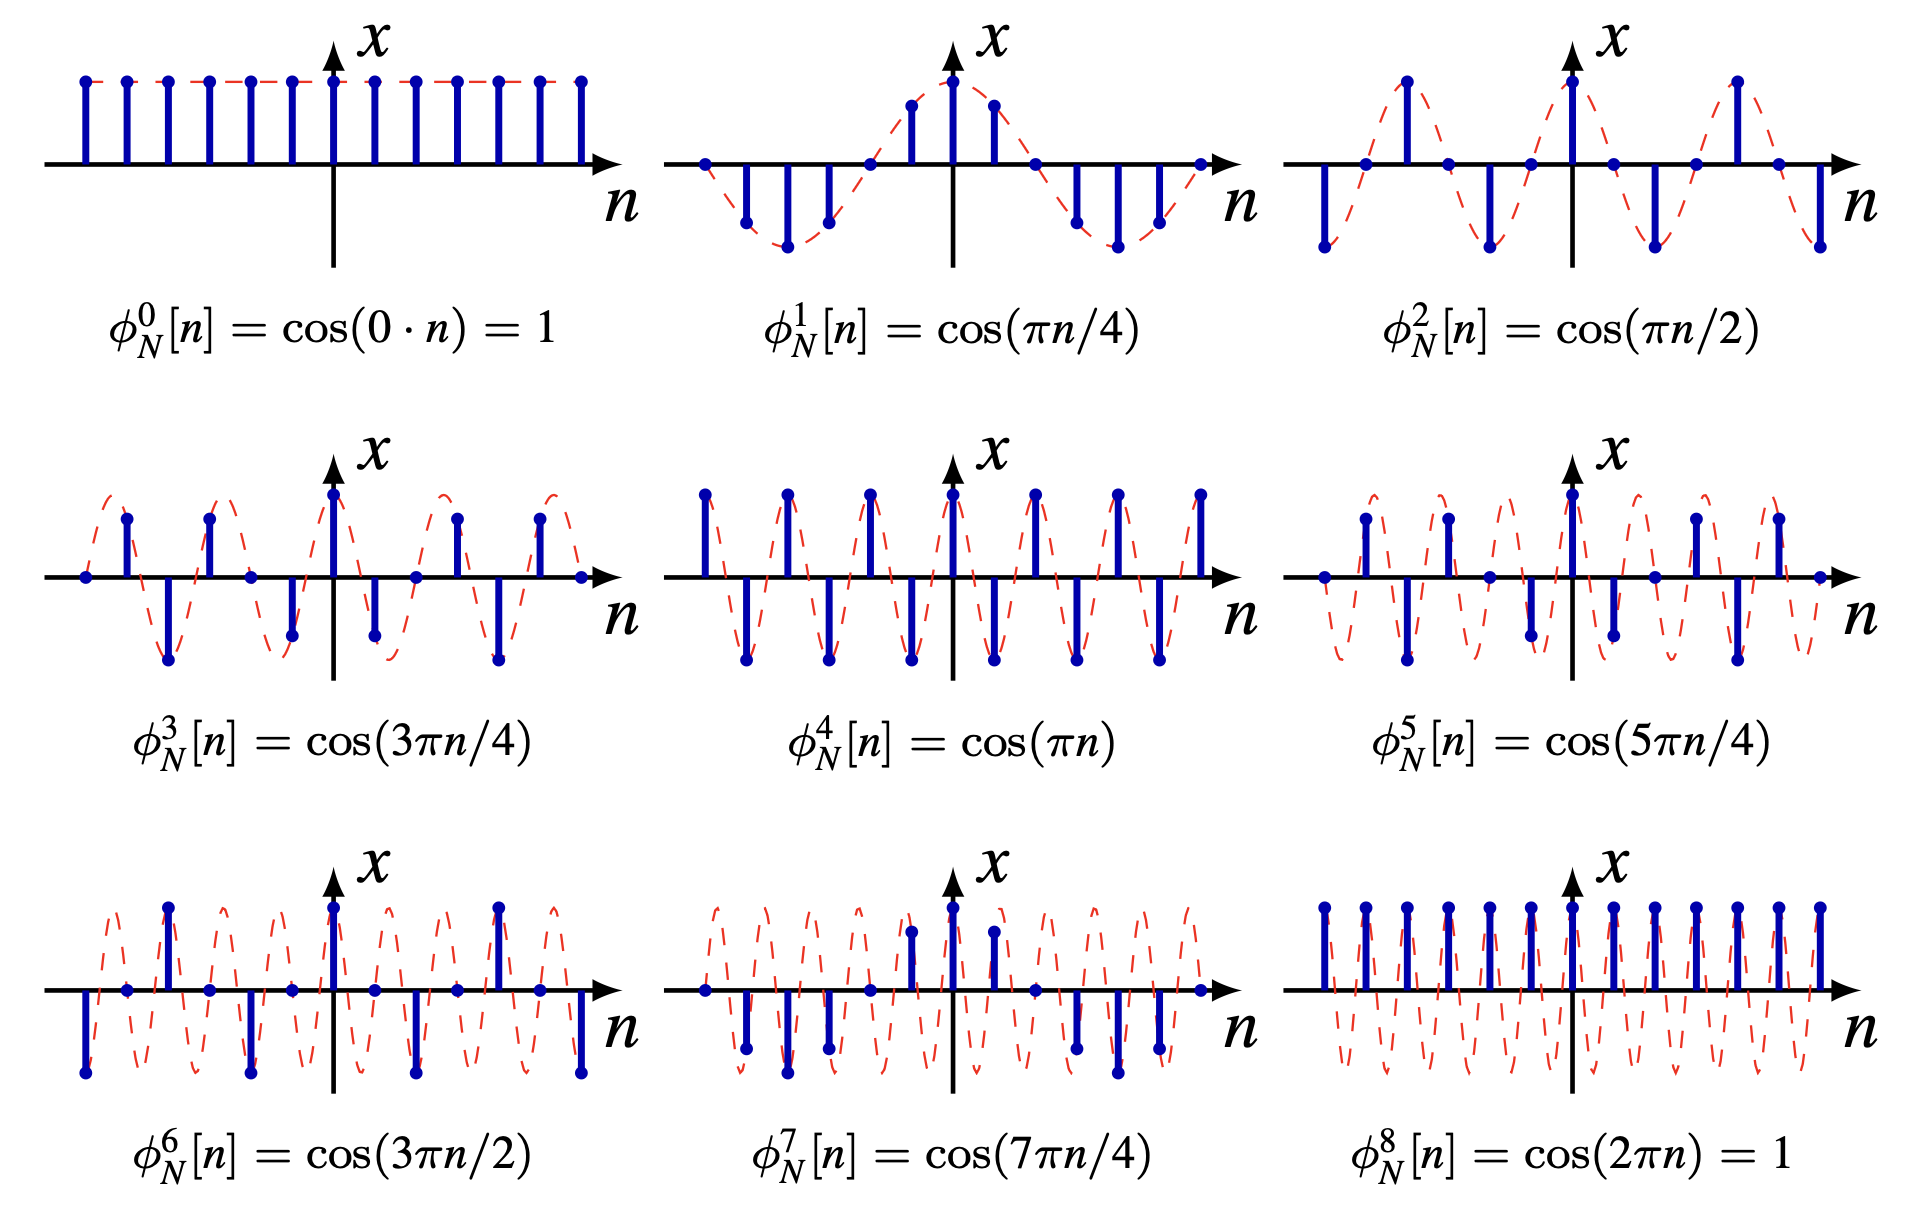
\includegraphics[keepaspectratio]{imglink/finitness.png}}
\end{center}
\end{frame}

\begin{frame}{谐波的正交归一性}
\protect\phantomsection\label{ux8c10ux6ce2ux7684ux6b63ux4ea4ux5f52ux4e00ux6027}
DT 傅里叶级数

\[
x=\sum_{k \in[N]} \hat{x}[k] \phi_{N}^{k}, \quad \text { 或 } \quad x[n]=\sum_{k \in[N]} \hat{x}[k] e^{j k \frac{2 \pi}{N} n}
\]

求和可以在任意 \(N\) 个连续整数上进行。 定义两个周期为 \(N\)
的信号的内积为

\[
\langle x, y\rangle=\frac{1}{N} \sum_{n \in[N]} x[n] \overline{y[n]}
\]

这与 \(\mathbb{C}^{N}\) 中的内积相同（差一个因子 \(N^{-1}\)）。
\(\left\{\phi_{N}^{k}: k \in[N]\right\}\) 是正交归一函数系

\[
\left\langle\phi_{N}^{k}, \phi_{N}^{m}\right\rangle=\delta_{k m}=\delta[k-m]
\]
\end{frame}

\begin{frame}{谐波正交归一性的证明}
\protect\phantomsection\label{ux8c10ux6ce2ux6b63ux4ea4ux5f52ux4e00ux6027ux7684ux8bc1ux660e}
\[
\left\langle\phi_{N}^{k}, \phi_{N}^{m}\right\rangle=\frac{1}{N} \sum_{n \in[N]} e^{j k \frac{2 \pi}{N} n} e^{-j m \frac{2 \pi}{N} n}=\frac{1}{N} \sum_{n=0}^{N-1} e^{j(k-m) \frac{2 \pi}{N} n}
\]

如果 \(k=m\)，

\[
\left\langle\phi_{N}^{k}, \phi_{N}^{m}\right\rangle=\frac{1}{N} \sum_{k=0}^{N-1} 1=1
\]

如果 \(k \neq m\)，由于
\(|k-m| \leq N-1, e^{j(k-m) \frac{2 \pi}{N}} \neq 1\)。利用等比数列求和公式：

\[
\left\langle\phi_{N}^{k}, \phi_{N}^{m}\right\rangle=\frac{1}{N} \sum_{n=0}^{N-1} e^{j(k-m) \frac{2 \pi}{N} n}=\frac{1}{N} \frac{1-e^{j(k-m) \frac{2 \pi}{N} N}}{1-e^{j(k-m) \frac{2 \pi}{N}}}=0
\]
\end{frame}

\begin{frame}{傅里叶系数}
\protect\phantomsection\label{ux5085ux91ccux53f6ux7cfbux6570}
假设 \(x\) 周期为 \(N\)，利用正交性求解系数：

\[
\begin{aligned}
\left\langle x, \phi_{N}^{m}\right\rangle & =\left\langle\sum_{k \in[N]} \hat{x}[k] \phi_{N}^{k}, \phi_{N}^{m}\right\rangle=\sum_{k \in[N]} \hat{x}[k]\left\langle\phi_{N}^{k}, \phi_{N}^{m}\right\rangle \\
& =\sum_{k \in[N]} \hat{x}[k] \delta[m-k]=\hat{x}[m]
\end{aligned}
\]

可以将 \(\hat{x}\) 视为 \(N\)-周期信号，因为：

\[
\hat{x}[m+r N] \triangleq\left\langle x, \phi_{N}^{m+r N}\right\rangle=\left\langle x, \phi_{N}^{m}\right\rangle=\hat{x}[m]
\]

但在傅里叶级数中只使用 \(N\) 个连续的值！
\end{frame}

\begin{frame}{DT 傅里叶级数公式}
\protect\phantomsection\label{dt-ux5085ux91ccux53f6ux7ea7ux6570ux516cux5f0f}
\textbf{综合方程 (Synthesis equation)}

\[
x[n]=\sum_{k \in[N]} \hat{x}[k] \phi_{N}^{k}[n]=\sum_{k \in[N]} \hat{x}[k] e^{j k \frac{2 \pi}{N} n}
\]

\textbf{分析方程 (Analysis equation)}

\[
\hat{x}[k]=\left\langle x, \phi_{N}^{k}\right\rangle=\frac{1}{N} \sum_{n \in[N]} x[n] e^{-j k \frac{2 \pi}{N} n}
\]

由于所有求和都是有限的，不存在收敛问题！
\end{frame}

\begin{frame}{例子}
\protect\phantomsection\label{ux4f8bux5b50-1}
\(x[n]=\cos \left(\frac{6 \pi}{5} n+\frac{\pi}{5}\right)\)，周期
\(N=5\)。 展开为复指数：
\(x[n]=\frac{e^{j \frac{\pi}{5}}}{2} e^{j 3 \frac{2 \pi}{5} n}+\frac{e^{-j \frac{\pi}{5}}}{2} e^{-j 3 \frac{2 \pi}{5} n}\)

系数：
\(\hat{x}[3]=\frac{1}{2} e^{j \frac{\pi}{5}} ; \quad \hat{x}[2]=\hat{x}[-3]=\frac{1}{2} e^{-j \frac{\pi}{5}} ; \quad \hat{x}[0]=\hat{x}[1]=\hat{x}[4]=0\)

\(\hat{x}[k]\) 以 \(N=5\) 为周期重复。

\begin{columns}[T]
\begin{column}{0.1\linewidth}
\[x[n]\]

\[|\hat{x}[n]|\]

\[Arg\hat{x}[n]\]
\end{column}

\begin{column}{0.9\linewidth}
\begin{center}
\pandocbounded{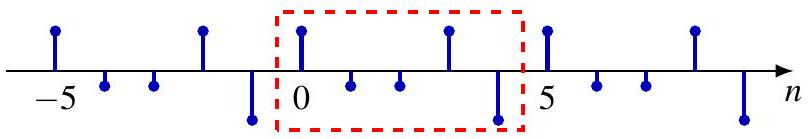
\includegraphics[keepaspectratio]{imglink/1086b18a-e1fd-43f2-95c8-7e053e314ef6-20.png}}
\end{center}

\begin{center}
\pandocbounded{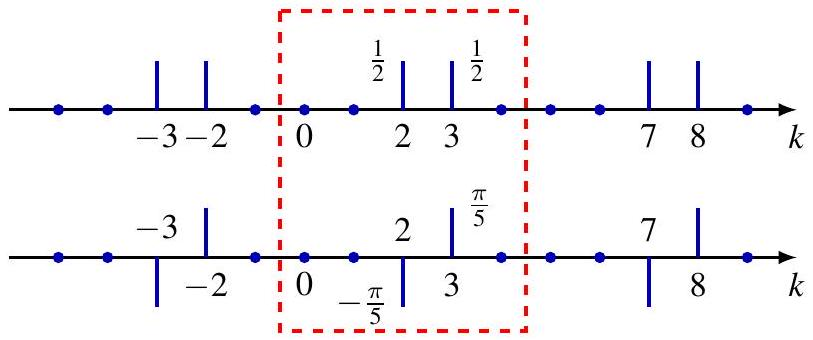
\includegraphics[keepaspectratio]{imglink/1086b18a-e1fd-43f2-95c8-7e053e314ef6-20_2.png}}
\end{center}
\end{column}
\end{columns}
\end{frame}

\begin{frame}{例子：周期方波 (Periodic Square Wave)}
\protect\phantomsection\label{ux4f8bux5b50ux5468ux671fux65b9ux6ce2-periodic-square-wave-1}
周期为 \(N\) 的方波，在一个周期内：

\[
x[n]= \begin{cases}1, & -N_{1} \leq n \leq N_{1} \\ 0, & N_{1}<n<N-N_{1}\end{cases}
\]

\pandocbounded{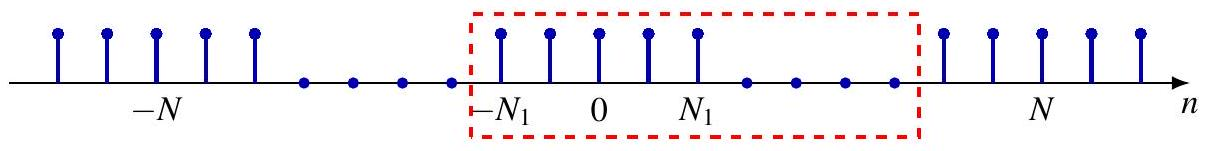
\includegraphics[keepaspectratio]{imglink/1086b18a-e1fd-43f2-95c8-7e053e314ef6-21.png}}

傅里叶系数：

\[
\hat{x}[k]=\frac{1}{N} \sum_{n=-N_{1}}^{N_{1}} e^{-j k \frac{2 \pi}{N} n}
\]

如果 \(k\) 是 \(N\) 的整数倍, \(\hat{x}[k]=\frac{2 N_{1}+1}{N}\)
\end{frame}

\begin{frame}{例子：周期方波 (续)}
\protect\phantomsection\label{ux4f8bux5b50ux5468ux671fux65b9ux6ce2-ux7eed}
如果 \(k\) 不是 \(N\) 的整数倍，则
\(e^{-j k \frac{2 \pi}{N}} \neq 1\)。使用等比数列求和：

\[
\begin{aligned}
\hat{x}[k] & =\frac{1}{N} \frac{e^{j k \frac{2 \pi}{N} N_{1}}-e^{-j k \frac{2 \pi}{N}\left(N_{1}+1\right)}}{1-e^{-j k \frac{2 \pi}{N}}} \\
& =\frac{1}{N} \frac{\sin \left(k \frac{2 \pi}{N}\left(N_{1}+\frac{1}{2}\right)\right)}{\sin \left(k \frac{\pi}{N}\right)}
\end{aligned}
\]

\pandocbounded{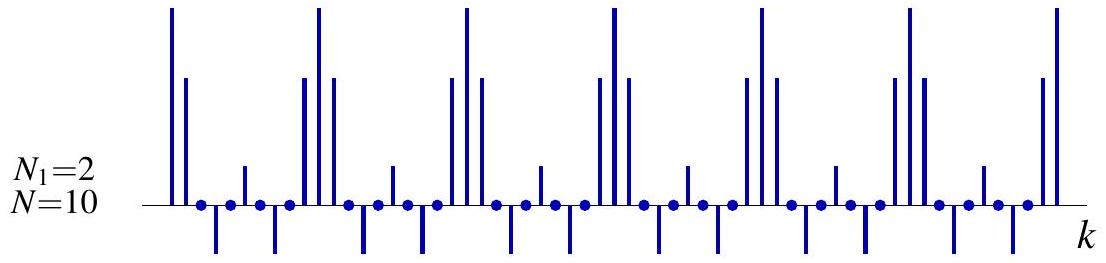
\includegraphics[keepaspectratio]{imglink/1086b18a-e1fd-43f2-95c8-7e053e314ef6-23.png}}
\end{frame}

\begin{frame}{DT 傅里叶级数：矩阵形式}
\protect\phantomsection\label{dt-ux5085ux91ccux53f6ux7ea7ux6570ux77e9ux9635ux5f62ux5f0f}
综合方程可以写成矩阵乘法：

\[
x[n]=\sum_{k=0}^{N-1} W_{N}^{k n} \hat{x}[k], \quad \text { 其中 } W_{N}=e^{j k \frac{2 \pi}{N}}
\]

\[
x=\mathbf{F} \hat{x}, \quad \text { 其中 } \mathbf{F}=\left(\phi_{N}^{0}, \phi_{N}^{1}, \ldots, \phi_{N}^{N-1}\right)
\]

分析方程：

\[
\hat{x}=\mathbf{F}^{-1} x=\frac{1}{N} \mathbf{F}^{H} x
\]

其中 \(\mathbf{F}^{H}=(\overline{\mathbf{F}})^{T}\) 是 \(\mathbf{F}\)
的共轭转置 (Hermitian transpose)。
\end{frame}

\begin{frame}{目录}
\protect\phantomsection\label{toc5}
\begin{itemize}
\tightlist
\item
  \hyperlink{sec31}{\textbf{1. 线性时不变系统对复指数信号的响应}}
\item
  \hyperlink{sec32}{2. 连续时间周期信号的傅里叶级数表示}
\item
  \hyperlink{sec33}{3. 连续时间傅里叶级数的收敛}
\item
  \hyperlink{sec34}{4. 连续时间傅里叶级数的性质}
\item
  \hyperlink{35}{5. 离散时间周期信号的傅里叶级数表示}
\item
  \hyperlink{sec36}{\textbf{6. 离散时间傅里叶级数的性质}}
\item
  \hyperlink{sec37}{7. 傅里叶级数与线性时不变系统}
\item
  \hyperlink{sec38}{8. 滤波}

  \begin{itemize}
  \tightlist
  \item
    \hyperlink{sec381}{频率成形滤波器}
  \item
    \hyperlink{sec382}{频率选择性滤波器}
  \item
    \hyperlink{sec383}{用微分方程描述的连续时间滤波器}
  \item
    \hyperlink{sec383}{用差分方程描述的离散时间滤波器}
  \end{itemize}
\end{itemize}
\end{frame}

\section{6. 离散时间傅里叶级数的性质}\label{sec36}

\begin{frame}{DT 傅里叶级数 (DT Fourier Series)}
\protect\phantomsection\label{dt-ux5085ux91ccux53f6ux7ea7ux6570-dt-fourier-series}
周期为 \(N\) 的信号 \(x\) 的 DTFS：

\[
x[n]=\sum_{k \in[N]} \hat{x}[k] e^{j k \omega_{0} n}, \quad \omega_{0}=\frac{2 \pi}{N}
\]

对应关系：

\[
x \stackrel{\text { DTFS }}{\longleftrightarrow} \hat{x} \quad \text { 或 } \quad x[n] \stackrel{\text { DTFS }}{\longleftrightarrow} \hat{x}[k]
\]

同一信号的两种等价表示： - 时域：\(x[n]\) - 频域：\(\hat{x}[k]\)
\end{frame}

\begin{frame}{线性、时移与频移}
\protect\phantomsection\label{ux7ebfux6027ux65f6ux79fbux4e0eux9891ux79fb}
\textbf{线性 (Linearity)} \[
\widehat{a x+b y}=a \hat{x}+b \hat{y}
\]

\textbf{时移 (Time shifting)} \[
x\left[n-n_{0}\right] \stackrel{\text { DTFS }}{\longleftrightarrow} e^{-j k \omega_{0} n_{0}} \hat{x}[k]
\]

\textbf{频移 (Frequency shifting)} \[
e^{j m \omega_{0} n} x[n] \stackrel{\text { DTFS }}{\longleftrightarrow} \hat{x}[k-m]
\]
\end{frame}

\begin{frame}{其它性质}
\protect\phantomsection\label{ux5176ux5b83ux6027ux8d28}
\textbf{时间反转 (Time reversal)} \[
x[-n] \stackrel{\text { DTFS }}{\longleftrightarrow} \hat{x}[-k]
\]

\textbf{共轭 (Conjugation)} \[
x^{*}[n] \stackrel{\text { DTFS }}{\longleftrightarrow}(\hat{x}[-k])^{*}
\]

\textbf{对称性 (Symmetry)} - \(x\) 实
\(\Longleftrightarrow \hat{x}[-k]=\overline{\hat{x}[k]}\) (共轭对称) -
\(x\) 实偶 \(\Longleftrightarrow \hat{x}\) 实偶
\end{frame}

\begin{frame}{时间缩放 (Time Scaling)}
\protect\phantomsection\label{ux65f6ux95f4ux7f29ux653e-time-scaling-1}
定义上采样信号 \(x_{(m)}\)：

\[
x_{(m)}[n]= \begin{cases}x[n / m], & \text { 如果 } n \text { 是 } m \text { 的倍数 } \\ 0, & \text { 其他 }\end{cases}
\]

如果 \(x\) 周期为 \(N\)，则 \(x_{(m)}\) 周期为 \(m N\)，且：

\[
\widehat{x_{(m)}}=\frac{1}{m} \hat{x} \quad \text { 或 } \quad x_{(m)}[n] \stackrel{\text { DTFS }}{\longleftrightarrow} \frac{1}{m} \hat{x}[k]
\]
\end{frame}

\begin{frame}{一阶差分与累加求和}
\protect\phantomsection\label{ux4e00ux9636ux5deeux5206ux4e0eux7d2fux52a0ux6c42ux548c}
\textbf{一阶（后向）差分} (First difference) \[
x[n]-x[n-1] \stackrel{\text { DTFS }}{\longleftrightarrow}\left(1-e^{-j k \frac{2 \pi}{N}}\right) \hat{x}[k]
\]

\textbf{累加求和} (Running sum) \[
y[n]=\sum_{m=n_{0}}^{n} x[m]
\] - \(y\) 是周期的当且仅当 \(\hat{x}[0]=0\)（无直流分量） - 如果
\(\hat{x}[0]=0\)， \[
\hat{y}[k]=\frac{1}{1-e^{-j k \frac{2 \pi}{N}}} \hat{x}[k] \quad \text { 对于 } k \neq 0
\]
\end{frame}

\begin{frame}{乘法 (Multiplication)}
\protect\phantomsection\label{ux4e58ux6cd5-multiplication-1}
时域乘法 \(\Longleftrightarrow\) 频域周期卷积

\[
x[n] y[n] \stackrel{\text { DTFS }}{\longleftrightarrow} \sum_{m \in[N]} \hat{x}[m] \hat{y}[k-m]
\]
\end{frame}

\begin{frame}{周期卷积 (Periodic Convolution)}
\protect\phantomsection\label{ux5468ux671fux5377ux79ef-periodic-convolution-1}
相同周期 \(N\) 的 \(x\) 和 \(y\) 的周期卷积：

\[
(x * y)[n]=\sum_{m \in[N]} x[m] y[n-m]
\]

性质： - 交换律、结合律、双线性

\textbf{时域卷积 \(\Longrightarrow\) 频域乘法}

\[
(x * y)[n] \stackrel{\text { DTFS }}{\longleftrightarrow} N \hat{x}[k] \hat{y}[k]
\]
\end{frame}

\begin{frame}{目录}
\protect\phantomsection\label{toc6}
\begin{itemize}
\tightlist
\item
  \hyperlink{sec31}{1. 线性时不变系统对复指数信号的响应}
\item
  \hyperlink{sec32}{2. 连续时间周期信号的傅里叶级数表示}
\item
  \hyperlink{sec33}{3. 连续时间傅里叶级数的收敛}
\item
  \hyperlink{sec34}{4. 连续时间傅里叶级数的性质}
\item
  \hyperlink{35}{5. 离散时间周期信号的傅里叶级数表示}
\item
  \hyperlink{sec36}{6. 离散时间傅里叶级数的性质}
\item
  \hyperlink{sec37}{\textbf{7. 傅里叶级数与线性时不变系统}}
\item
  \hyperlink{sec38}{8. 滤波}

  \begin{itemize}
  \tightlist
  \item
    \hyperlink{sec381}{频率成形滤波器}
  \item
    \hyperlink{sec382}{频率选择性滤波器}
  \item
    \hyperlink{sec383}{用微分方程描述的连续时间滤波器}
  \item
    \hyperlink{sec383}{用差分方程描述的离散时间滤波器}
  \end{itemize}
\end{itemize}
\end{frame}

\section{7. 傅里叶级数与线性时不变系统}\label{sec37}

\begin{frame}{目录}
\protect\phantomsection\label{toc7}
\begin{itemize}
\tightlist
\item
  \hyperlink{sec31}{1. 线性时不变系统对复指数信号的响应}
\item
  \hyperlink{sec32}{2. 连续时间周期信号的傅里叶级数表示}
\item
  \hyperlink{sec33}{3. 连续时间傅里叶级数的收敛}
\item
  \hyperlink{sec34}{4. 连续时间傅里叶级数的性质}
\item
  \hyperlink{35}{5. 离散时间周期信号的傅里叶级数表示}
\item
  \hyperlink{sec36}{6. 离散时间傅里叶级数的性质}
\item
  \hyperlink{sec37}{7. 傅里叶级数与线性时不变系统}
\item
  \hyperlink{sec38}{\textbf{8. 滤波}}

  \begin{itemize}
  \tightlist
  \item
    \hyperlink{sec381}{频率成形滤波器}
  \item
    \hyperlink{sec382}{频率选择性滤波器}
  \item
    \hyperlink{sec383}{用微分方程描述的连续时间滤波器}
  \item
    \hyperlink{sec383}{用差分方程描述的离散时间滤波器}
  \end{itemize}
\end{itemize}
\end{frame}

\section{8. 滤波}\label{sec38}

\begin{frame}{频率成形滤波器}
\protect\phantomsection\label{sec381}
\end{frame}

\begin{frame}{频率响应}
\protect\phantomsection\label{ux9891ux7387ux54cdux5e94}
回顾连续时间（CT）线性时不变（LTI）系统对指数输入 \(e^{st}\) 的响应：

\[T \left( \sum_{k} a_k e^{s_k t} \right) = \sum_{k} a_k H(s_k) e^{s_k t}\]

其中 \(H(s)\) 是\textbf{系统函数}（System Function）：

\[H(s) = \int_{\mathbb{R}} h(t) e^{-st} dt\]

当限定 \(s = j\omega\) 时，\(H(j\omega)\) 作为 \(\omega\)
的函数被称为系统的\textbf{频率响应}（Frequency Response）：

\[H(j\omega) = \int_{\mathbb{R}} h(t) e^{-j\omega t} dt\]
\end{frame}

\begin{frame}{滤波}
\protect\phantomsection\label{ux6ee4ux6ce2}
傅里叶级数表示下的周期输入 \(x\)：

\[x(t) = \sum_{k=-\infty}^{\infty} \hat{x}[k] e^{jk\omega_0 t}\]

具有频率响应 \(H(j\omega)\) 的 LTI 系统的输出：

\[y(t) = T \left( \sum_{k=-\infty}^{\infty} \hat{x}[k] e^{jk\omega_0 t} \right) = \sum_{k=-\infty}^{\infty} H(j k \omega_0) \hat{x}[k] e^{j k \omega_0 t}\]

输出信号是周期性的且具有相同的周期，其傅里叶系数的关系为：

\[\hat{y}[k] = H(j k \omega_0) \hat{x}[k]\]

\textbf{滤波}会改变频率分量的相对幅度，或者完全消除某些频率分量。
\end{frame}

\begin{frame}{滤波}
\protect\phantomsection\label{ux6ee4ux6ce2-1}
\begin{columns}[T]
\begin{column}{0.5\linewidth}
\textbf{示例}：微分器 \(T(x) = x'\) 的频率响应为：

\[H(j\omega) = j\omega\]

对于周期输入信号：

\[x(t) = \sum_{k=-\infty}^{\infty} \hat{x}[k] e^{jk\omega_0 t}\]

其输出信号为：

\[y(t) = \sum_{k=-\infty}^{\infty} jk\omega_0 \hat{x}[k] e^{jk\omega_0 t}\]

傅里叶系数的关系如下：

\[\hat{y}[k] = jk\omega_0 \hat{x}[k]\]
\end{column}

\begin{column}{0.5\linewidth}
\pandocbounded{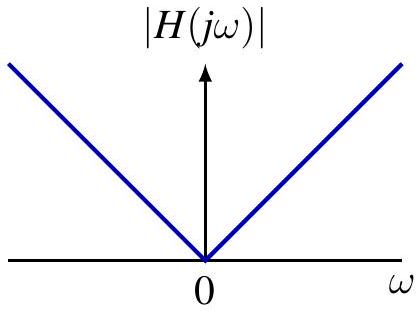
\includegraphics[keepaspectratio]{imglink/4cb8e742-a9ce-42fa-a004-42de4559e768-31.png}}

\pandocbounded{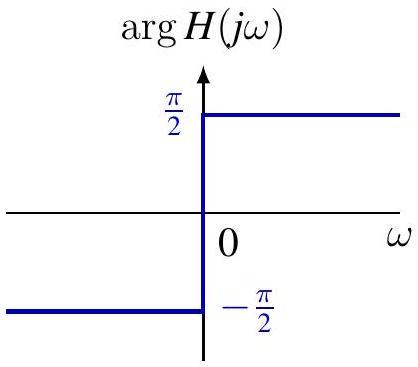
\includegraphics[keepaspectratio]{imglink/4cb8e742-a9ce-42fa-a004-42de4559e768-31_2.png}}
\end{column}
\end{columns}
\end{frame}

\begin{frame}{滤波}
\protect\phantomsection\label{ux6ee4ux6ce2-2}
\begin{itemize}
\tightlist
\item
  \textbf{不能}产生新的频率分量。
\item
  \textbf{只能}缩放现有分量的幅度或移动其相位。
\end{itemize}

\textbf{非线性滤波器示例：} 削波（Clipping）
\(y(t) = \max\{x(t), c\}\)。\\
\emph{本课程重点关注 \textbf{LTI 滤波器}。}

\begin{block}{频率整形滤波器 (Frequency-shaping filters)}
\protect\phantomsection\label{ux9891ux7387ux6574ux5f62ux6ee4ux6ce2ux5668-frequency-shaping-filters}
这类滤波器会改变频谱的形状。

\begin{itemize}
\tightlist
\item
  \textbf{例如：均衡器 (Equalizer)}
\end{itemize}

\pandocbounded{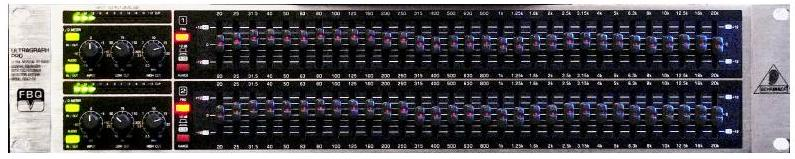
\includegraphics[keepaspectratio]{imglink/4cb8e742-a9ce-42fa-a004-42de4559e768-32.png}}
\end{block}

\begin{block}{频率选择性滤波器 (Frequency-selective filters)}
\protect\phantomsection\label{ux9891ux7387ux9009ux62e9ux6027ux6ee4ux6ce2ux5668-frequency-selective-filters}
这类滤波器使某些频率基本无失真地通过，并显著衰减或消除其他频率。
\end{block}
\end{frame}

\begin{frame}{理想频率选择性滤波器}
\protect\phantomsection\label{ux7406ux60f3ux9891ux7387ux9009ux62e9ux6027ux6ee4ux6ce2ux5668}
\begin{columns}[T]
\begin{column}{0.33\linewidth}
理想低通滤波器

\[
H(j \omega)= \begin{cases}1, & |\omega| \leq \omega_{c} \\ 0, & \text { 其他 }\end{cases}
\]

\(\omega_{c}\) : 截止频率
\pandocbounded{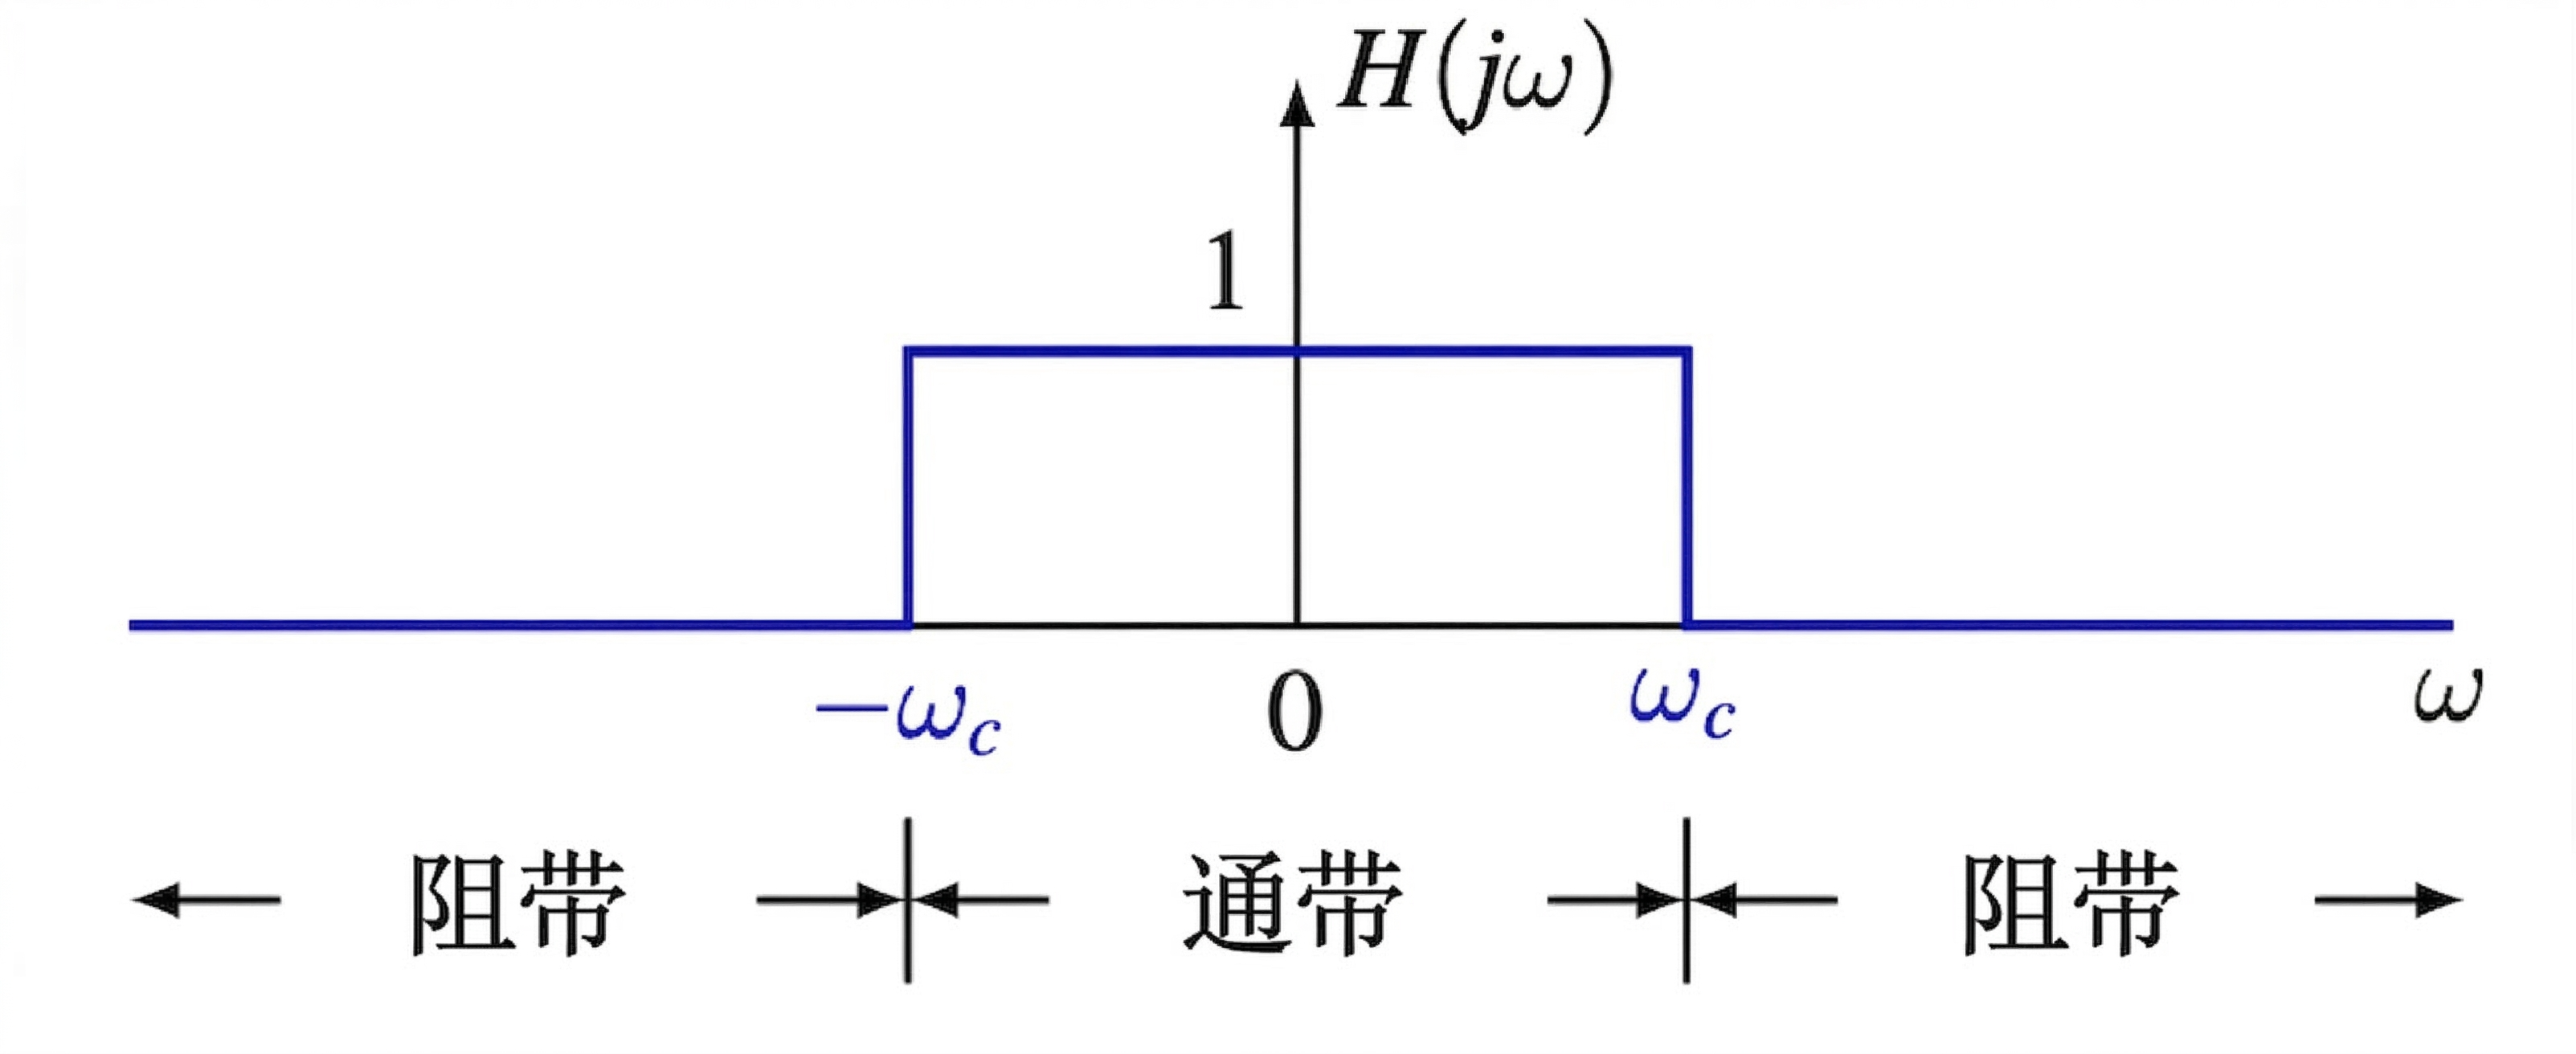
\includegraphics[keepaspectratio]{imglink/ideallowpassfilter.png}}
\end{column}

\begin{column}{0.34\linewidth}
理想高通滤波器

\[
H(j \omega)= \begin{cases}1, & |\omega| \geq \omega_{c} \\ 0, & \text { otherwise }\end{cases}
\]

\(\omega_{c}\) : 截止频率
\pandocbounded{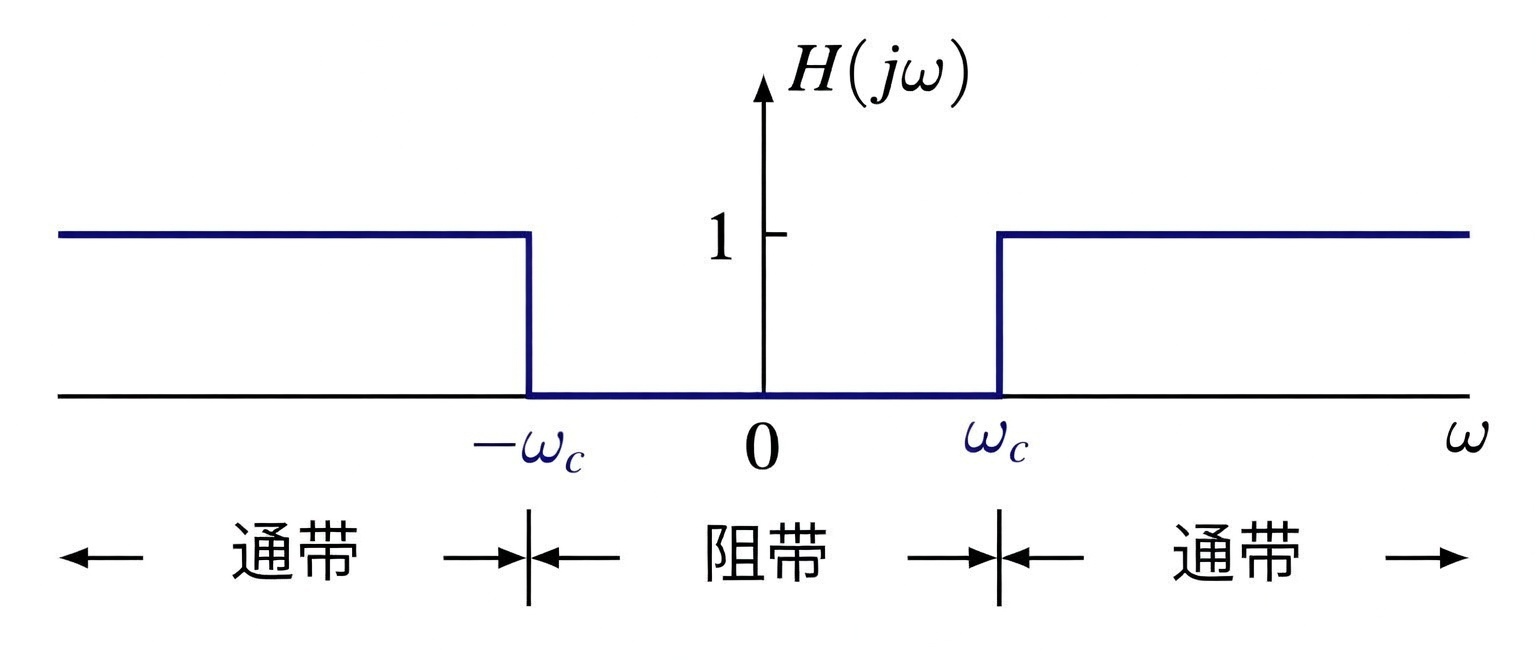
\includegraphics[keepaspectratio]{imglink/idealhighpassfilter.png}}
\end{column}

\begin{column}{0.33\linewidth}
理想带通滤波器

\[
H(j \omega)= \begin{cases}1, & \omega_{c 1} \leq|\omega| \leq \omega_{c 2} \\ 0, & \text { otherwise }\end{cases}
\]

\(\omega_{c 1}\) : 下截止频率， \(\omega_{c 2}\) : 上截止频率
\pandocbounded{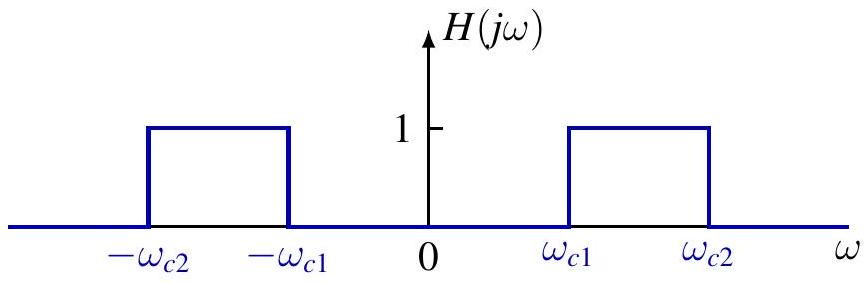
\includegraphics[keepaspectratio]{imglink/4cb8e742-a9ce-42fa-a004-42de4559e768-35.png}}
\end{column}
\end{columns}
\end{frame}

\begin{frame}{用微分方程描述的连续时间滤波器}
\protect\phantomsection\label{sec383}
\begin{block}{简单 RC 低通滤波器}
\protect\phantomsection\label{ux7b80ux5355-rc-ux4f4eux901aux6ee4ux6ce2ux5668}
\begin{columns}[T]
\begin{column}{0.5\linewidth}
常微分方程 (ODE)

\[
R C \frac{d v_{C}(t)}{d t}+v_{C}(t)=v_{S}(t)
\]

对于输入 \(v_{S}(t)=e^{j \omega t}\)，输出为

\[
v_{C}(t)=H(j \omega) e^{j \omega t}
\]

频率响应 \(H(j \omega)=\frac{1}{1+R C j \omega}\)
\end{column}

\begin{column}{0.5\linewidth}
\pandocbounded{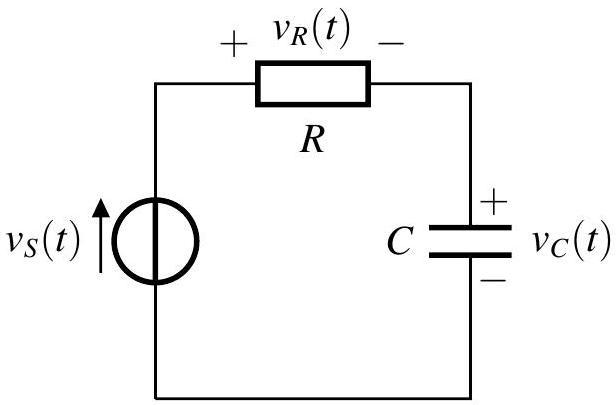
\includegraphics[keepaspectratio]{imglink/1086b18a-e1fd-43f2-95c8-7e053e314ef6-06.png}}
\end{column}
\end{columns}
\end{block}
\end{frame}

\begin{frame}{简单 RC 低通滤波器}
\protect\phantomsection\label{ux7b80ux5355-rc-ux4f4eux901aux6ee4ux6ce2ux5668-1}
\begin{columns}[T]
\begin{column}{0.5\linewidth}
频率响应

\[
H(j \omega)=\frac{1}{1+R C j \omega}
\]

\[
\begin{aligned}
|H(j \omega)| & =\frac{1}{\sqrt{1+(R C \omega)^{2}}} \\
\arg H(j \omega) & =-\arctan (R C \omega)
\end{aligned}
\] 非理想低通滤波器：通过低频，衰减高频。

\(R C\) 越大 \(\Longrightarrow\) 通过的低频范围越小。
\end{column}

\begin{column}{0.5\linewidth}
\pandocbounded{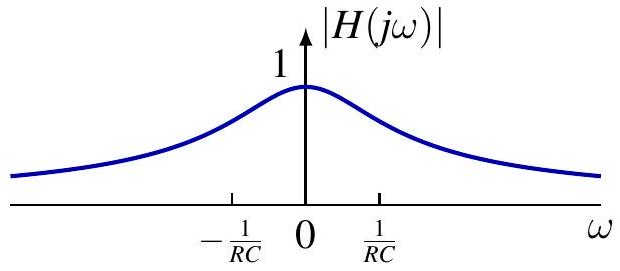
\includegraphics[keepaspectratio]{imglink/1086b18a-e1fd-43f2-95c8-7e053e314ef6-07.png}}

\pandocbounded{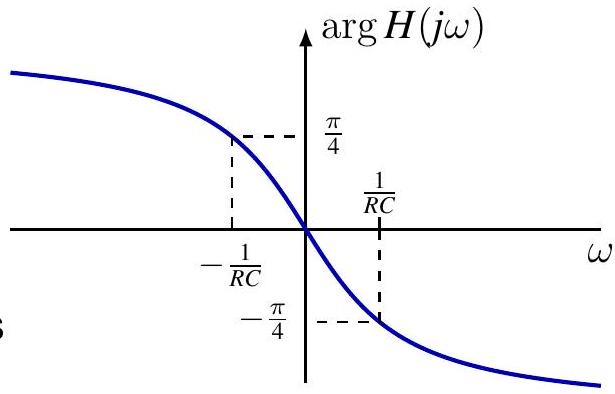
\includegraphics[keepaspectratio]{imglink/1086b18a-e1fd-43f2-95c8-7e053e314ef6-07_2.png}}
\end{column}
\end{columns}
\end{frame}

\begin{frame}{简单 RC 低通滤波器}
\protect\phantomsection\label{ux7b80ux5355-rc-ux4f4eux901aux6ee4ux6ce2ux5668-2}
\begin{columns}[T]
\begin{column}{0.5\linewidth}
冲激响应

\[
h(t)=\frac{1}{R C} e^{-t / R C} u(t)
\]

阶跃响应

\[
s(t)=(h * u)(t)=\left(1-e^{-t / R C}\right) u(t)
\]

时间常数 \(\tau=R C\)

\begin{itemize}
\tightlist
\item
  \(\tau\) 越大，响应越迟缓 (sluggish)
\end{itemize}
\end{column}

\begin{column}{0.5\linewidth}
\pandocbounded{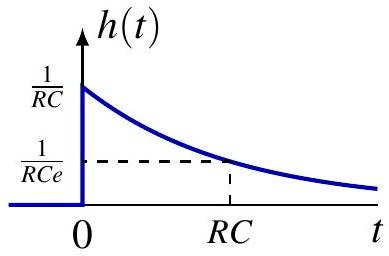
\includegraphics[keepaspectratio]{imglink/1086b18a-e1fd-43f2-95c8-7e053e314ef6-08.png}}

\pandocbounded{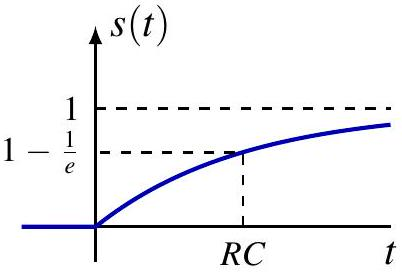
\includegraphics[keepaspectratio]{imglink/1086b18a-e1fd-43f2-95c8-7e053e314ef6-08_2.png}}
\end{column}
\end{columns}

\begin{block}{权衡 (Tradeoff)}
\protect\phantomsection\label{ux6743ux8861-tradeoff}
\begin{itemize}
\tightlist
\item
  \(\tau\) 越大：通过的高频越少，响应越迟缓
\item
  \(\tau\) 越小：通过的高频越多，响应越快
\end{itemize}
\end{block}
\end{frame}

\begin{frame}{简单 RC 高通滤波器}
\protect\phantomsection\label{ux7b80ux5355-rc-ux9ad8ux901aux6ee4ux6ce2ux5668}
\begin{columns}[T]
\begin{column}{0.5\linewidth}
ODE \(R C \frac{d v_{R}(t)}{d t}+v_{R}(t)=R C \frac{d v_{S}(t)}{d t}\)

对于输入 \(v_{S}(t)=e^{j \omega t}\)，输出为

\[
v_{R}(t)=H(j \omega) e^{j \omega t}
\]

频率响应 \(\quad H(j \omega)=\frac{j \omega R C}{1+j \omega R C}\)
\end{column}

\begin{column}{0.5\linewidth}
\pandocbounded{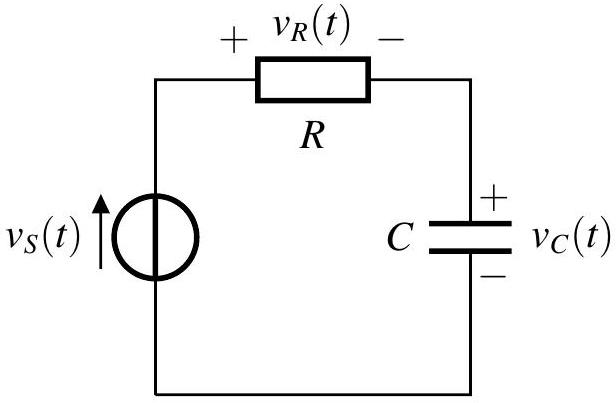
\includegraphics[keepaspectratio]{imglink/1086b18a-e1fd-43f2-95c8-7e053e314ef6-09.png}}
\end{column}
\end{columns}
\end{frame}

\begin{frame}{简单 RC 高通滤波器}
\protect\phantomsection\label{ux7b80ux5355-rc-ux9ad8ux901aux6ee4ux6ce2ux5668-1}
\begin{columns}[T]
\begin{column}{0.5\linewidth}
频率响应

\[
H(j \omega)=\frac{j \omega R C}{1+j \omega R C}
\]

\[
|H(j \omega)|=\frac{|\omega| R C}{\sqrt{1+(R C \omega)^{2}}}
\]

\[
\arg H(j \omega)=\arctan \frac{1}{R C \omega}
\]

非理想高通滤波器：通过高频，衰减低频。

\(R C\) 越大 \(\Longrightarrow\) 通过的低频范围越大。
\end{column}

\begin{column}{0.5\linewidth}
\pandocbounded{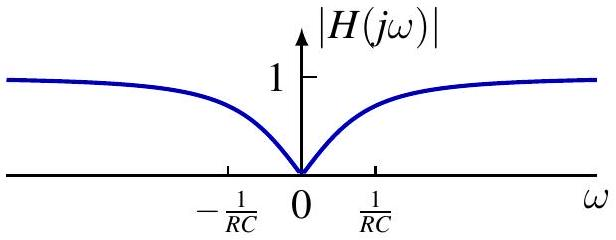
\includegraphics[keepaspectratio]{imglink/1086b18a-e1fd-43f2-95c8-7e053e314ef6-10.png}}

\pandocbounded{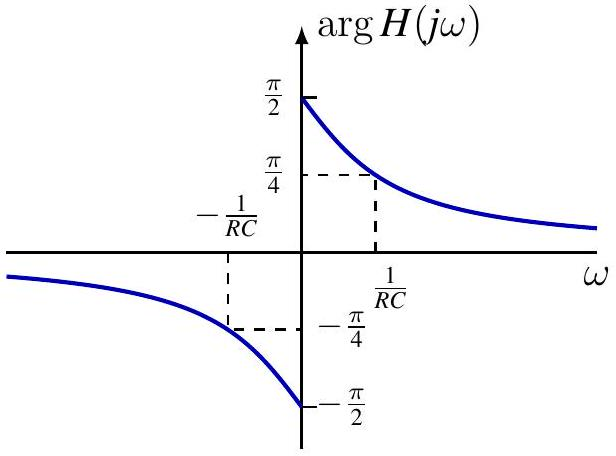
\includegraphics[keepaspectratio]{imglink/1086b18a-e1fd-43f2-95c8-7e053e314ef6-10_2.png}}
\end{column}
\end{columns}
\end{frame}

\begin{frame}{简单 RC 高通滤波器}
\protect\phantomsection\label{ux7b80ux5355-rc-ux9ad8ux901aux6ee4ux6ce2ux5668-2}
\begin{columns}[T]
\begin{column}{0.5\linewidth}
阶跃响应

\[
s(t)=e^{-t / R C} u(t)
\]

冲激响应

\[
h(t)=s^{\prime}(t)=\delta(t)-\frac{1}{R C} e^{-t / R C} u(t)
\]

时间常数 \(\tau=R C\)

\begin{itemize}
\tightlist
\item
  \(\tau\) 越大，响应越迟缓
\end{itemize}
\end{column}

\begin{column}{0.5\linewidth}
\pandocbounded{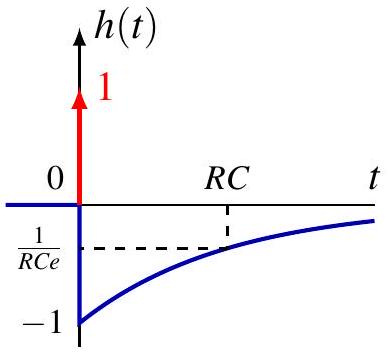
\includegraphics[keepaspectratio]{imglink/1086b18a-e1fd-43f2-95c8-7e053e314ef6-11_2.png}}

\pandocbounded{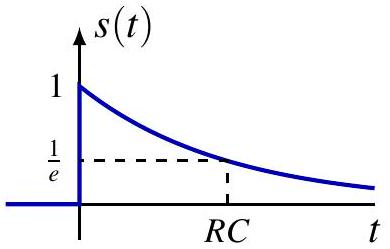
\includegraphics[keepaspectratio]{imglink/1086b18a-e1fd-43f2-95c8-7e053e314ef6-11.png}}
\end{column}
\end{columns}

观察： - \(\tau\) 越大，通过的低频越多，响应越迟缓 - \(\tau\)
越小，通过的低频越少，响应越快
\end{frame}

\begin{frame}{用差分方程描述的连续时间滤波器}
\protect\phantomsection\label{sec384}
\begin{columns}[T]
\begin{column}{0.5\linewidth}
\(N\)-周期序列离散时间傅里叶级数（Discrete Time Fourier Series,
DTFS）变换对

\textbf{分析公式}

\[
\hat{x}[k]=\frac{1}{N} \sum_{n \in[N]} x[n] e^{-j k \frac{2 \pi}{N} n}
\]

\textbf{综合公式}

\[
x[n]=\sum_{k \in[N]} \hat{x}[k] e^{j k \frac{2 \pi}{N} n}
\]
\end{column}

\begin{column}{0.5\linewidth}
有限长度\(N\)序列的离散傅里叶变换（Discrete Fourier Tranform,
DFT）对(详细内容见第五章)

\textbf{DFT}

\[
X[k]=\sum_{n=0}^{N-1} x[n] e^{-j k \frac{2 \pi}{N} n}
\]

\textbf{逆 DFT}

\[
x[n]=\frac{1}{N} \sum_{k=0}^{N-1} X[k] e^{j k \frac{2 \pi}{N} n}
\]
\end{column}
\end{columns}

这两组方程本质上是相同的，差别仅在于一个常数因子\(\frac{1}{N}\);
都可以通过\textbf{快速傅里叶变换 (FFT)}实现高效计算
\end{frame}

\begin{frame}{频率响应}
\protect\phantomsection\label{ux9891ux7387ux54cdux5e94-1}
回顾离散时间 (DT) 线性时不变量 (LTI) 系统对指数输入 \(z^n\) 的响应：

\[T\left( \sum_{k} a_k z_k^n \right) = \sum_{k} a_k H(z_k) z_k^n\]

其中 \(H(z)\) 是\textbf{系统函数}：

\[H(z) = \sum_{n=-\infty}^{\infty} h[n] z^{-n}\]

当限定 \(z = e^{j\omega}\) 时，\(H(e^{j\omega})\) 作为 \(\omega\)
的函数被称为系统的\textbf{频率响应}：

\[H(e^{j\omega}) = \sum_{n=-\infty}^{\infty} h[n] e^{-j\omega n}\]
\end{frame}

\begin{frame}{频率响应}
\protect\phantomsection\label{ux9891ux7387ux54cdux5e94-2}
周期输入 \(x\) 的傅里叶级数表示：

\[x[n] = \sum_{k \in [N]} \hat{x}[k] e^{j k \omega_0 n}, \quad \text{其中 } \omega_0 = \frac{2\pi}{N}\]

频率响应为 \(H(e^{j\omega})\) 的 LTI 系统的输出：

\[y[n] = T \left( \sum_{k \in [N]} \hat{x}[k] e^{j k \omega_0 n} \right) = \sum_{k \in [N]} H(e^{j k \omega_0}) \hat{x}[k] e^{j k \omega_0 n}\]

输出信号具有相同的周期，其傅里叶系数之间的关系为：

\[\hat{y}[k] = H(e^{j k \omega_0}) \hat{x}[k]\]
\end{frame}

\begin{frame}{滤波}
\protect\phantomsection\label{ux6ee4ux6ce2-3}
\textbf{滤波}会改变频率分量的相对幅度，或者完全消除某些频率分量。

\begin{block}{LTI 系统作为滤波器}
\protect\phantomsection\label{lti-ux7cfbux7edfux4f5cux4e3aux6ee4ux6ce2ux5668}
在线性时不变量 (LTI) 系统中，正如连续时间 (CT)
情况一样，系统扮演着滤波器的角色。频率整形 (Frequency-shaping)
与频率选择性 (Frequency-selective) 滤波器的共同点在于：

\begin{itemize}
\tightlist
\item
  \textbf{无法创造}新的频率分量。
\item
  \textbf{只能缩放}现有分量的幅度或偏移其相位。
\end{itemize}
\end{block}

\begin{block}{非线性滤波器示例 (Examples of Nonlinear Filter)}
\protect\phantomsection\label{ux975eux7ebfux6027ux6ee4ux6ce2ux5668ux793aux4f8b-examples-of-nonlinear-filter}
非线性滤波器不遵循 LTI 系统的上述限制，可以产生新的频率分量。

\begin{itemize}
\tightlist
\item
  \textbf{极大值滤波器 (Max filter)}:
  \[y[n] = \max_{-n_1 \leq k \leq n_2} x[n + k]\]
\item
  \textbf{中值滤波器 (Median filter)}:
  \[y[n] = \text{median} \{x[n - n_1], \dots, x[n + n_2]\}\]
\end{itemize}
\end{block}

\begin{block}{离散时间 (DT) 信号的频率}
\protect\phantomsection\label{ux79bbux6563ux65f6ux95f4-dt-ux4fe1ux53f7ux7684ux9891ux7387}
回顾离散时间信号的特性：只需考虑长度为 \(2\pi\) 的频率区间即可，例如
\([0, 2\pi)\) 或 \((-\pi, \pi]\)。
\end{block}
\end{frame}

\begin{frame}{离散时间信号中的高频与低频}
\protect\phantomsection\label{ux79bbux6563ux65f6ux95f4ux4fe1ux53f7ux4e2dux7684ux9ad8ux9891ux4e0eux4f4eux9891}
高频分布在 \((2k + 1)\pi\) 附近，低频分布在 \(2k\pi\) 附近。

\begin{columns}[T]
\begin{column}{0.33\linewidth}
\pandocbounded{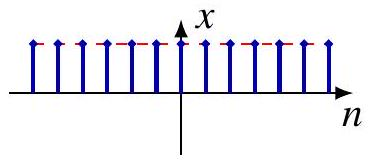
\includegraphics[keepaspectratio]{imglink/f0d10ac8-9b51-40af-8373-7a211a98e620-13_7.png}}

\(\phi_{N}^{0}[n]=\cos (0 \cdot n)=1\)

\pandocbounded{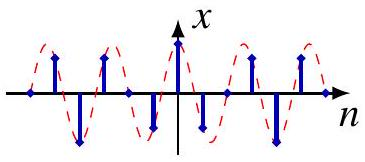
\includegraphics[keepaspectratio]{imglink/f0d10ac8-9b51-40af-8373-7a211a98e620-13_9.png}}

\(\phi_{N}^{3}[n]=\cos (3 \pi n / 4)\)

\pandocbounded{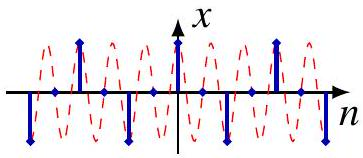
\includegraphics[keepaspectratio]{imglink/f0d10ac8-9b51-40af-8373-7a211a98e620-13_3.png}}

\(\phi_{N}^{6}[n]=\cos (3 \pi n / 2)\)
\end{column}

\begin{column}{0.34\linewidth}
\pandocbounded{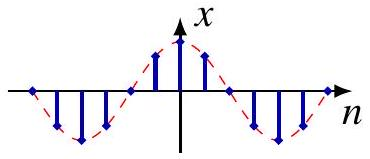
\includegraphics[keepaspectratio]{imglink/f0d10ac8-9b51-40af-8373-7a211a98e620-13_5.png}}

\(\phi_{N}^{1}[n]=\cos (\pi n / 4)\)

\pandocbounded{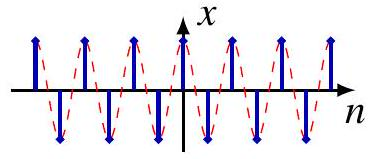
\includegraphics[keepaspectratio]{imglink/f0d10ac8-9b51-40af-8373-7a211a98e620-13_6.png}}

\(\phi_{N}^{4}[n]=\cos (\pi n)\)

\pandocbounded{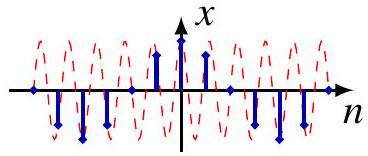
\includegraphics[keepaspectratio]{imglink/f0d10ac8-9b51-40af-8373-7a211a98e620-13_2.png}}

\(\phi_{N}^{7}[n]=\cos (7 \pi n / 4)\)
\end{column}

\begin{column}{0.33\linewidth}
\pandocbounded{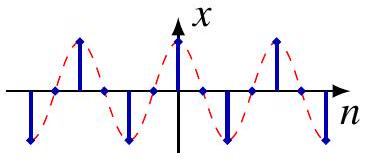
\includegraphics[keepaspectratio]{imglink/f0d10ac8-9b51-40af-8373-7a211a98e620-13_4.png}}

\(\phi_{N}^{2}[n]=\cos (\pi n / 2)\)

\pandocbounded{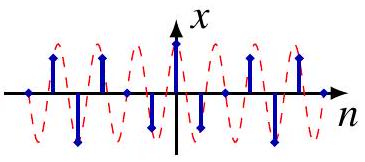
\includegraphics[keepaspectratio]{imglink/f0d10ac8-9b51-40af-8373-7a211a98e620-13_8.png}}

\(\phi_{N}^{5}[n]=\cos (5 \pi n / 4)\)

\pandocbounded{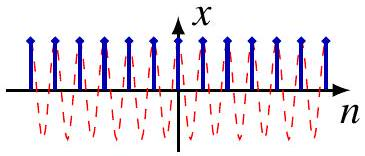
\includegraphics[keepaspectratio]{imglink/f0d10ac8-9b51-40af-8373-7a211a98e620-13.png}}

\(\phi_{N}^{8}[n]=\cos (2 \pi n)=1\)
\end{column}
\end{columns}
\end{frame}

\begin{frame}{离散时间频率}
\protect\phantomsection\label{ux79bbux6563ux65f6ux95f4ux9891ux7387}
\(N\) 周期信号的离散频率特性：

\begin{itemize}
\tightlist
\item
  \textbf{单位圆上的等间隔点}：频率分量均匀分布在复平面的单位圆上。
\item
  \textbf{低频靠近 \(1\)，高频靠近 \(-1\)}：

  \begin{itemize}
  \tightlist
  \item
    当 \(z = e^{j\omega} \approx 1\)（即
    \(\omega \approx 2k\pi\)）时，对应低频。
  \item
    当 \(z = e^{j\omega} \approx -1\)（即
    \(\omega \approx (2k+1)\pi\)）时，对应高频。
  \end{itemize}
\end{itemize}

\begin{columns}[T]
\begin{column}{0.5\linewidth}
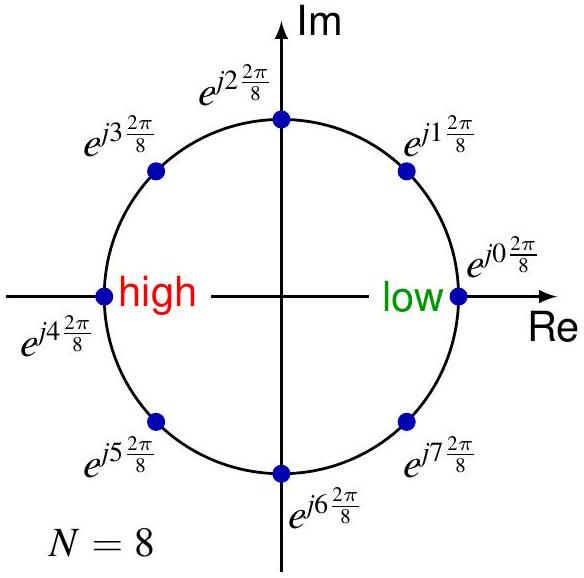
\includegraphics[width=0.6\linewidth,height=\textheight,keepaspectratio]{imglink/f0d10ac8-9b51-40af-8373-7a211a98e620-14.png}
\end{column}

\begin{column}{0.5\linewidth}
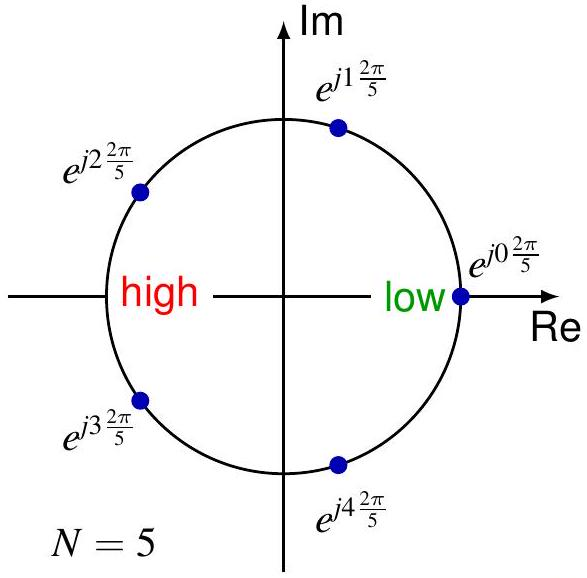
\includegraphics[width=0.6\linewidth,height=\textheight,keepaspectratio]{imglink/f0d10ac8-9b51-40af-8373-7a211a98e620-14_2.png}
\end{column}
\end{columns}
\end{frame}

\begin{frame}{理想频率选择性滤波器}
\protect\phantomsection\label{ux7406ux60f3ux9891ux7387ux9009ux62e9ux6027ux6ee4ux6ce2ux5668-1}
理想低通滤波器

\[
H\left(e^{j \omega}\right)= \begin{cases}1, & |\omega| \leq \omega_{c} \\ 0, & \omega_{c}<|\omega| \leq \pi\end{cases}
\]

\(\omega_{c}\) : 截止频率

\pandocbounded{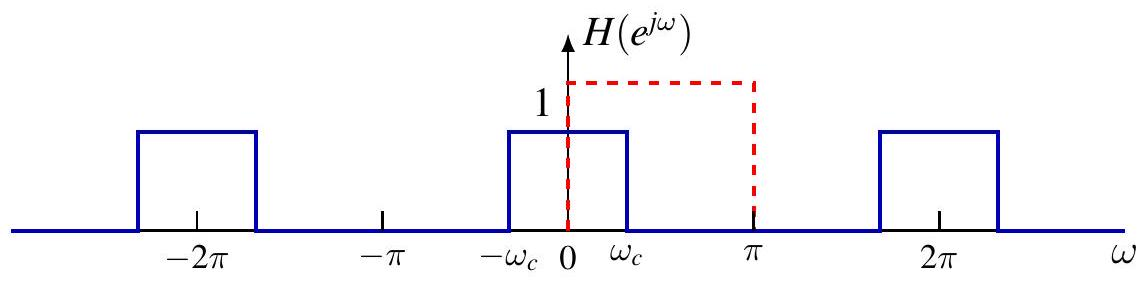
\includegraphics[keepaspectratio]{imglink/f0d10ac8-9b51-40af-8373-7a211a98e620-15.png}}
\end{frame}

\begin{frame}{理想频率选择性滤波器}
\protect\phantomsection\label{ux7406ux60f3ux9891ux7387ux9009ux62e9ux6027ux6ee4ux6ce2ux5668-2}
理想高通滤波器

\[
H\left(e^{j \omega}\right)= \begin{cases}1, & \omega_{c} \leq|\omega| \leq \pi \\ 0, & |\omega|<\left|\omega_{c}\right|\end{cases}
\]

\(\omega_{c}\) : 截止频率

\pandocbounded{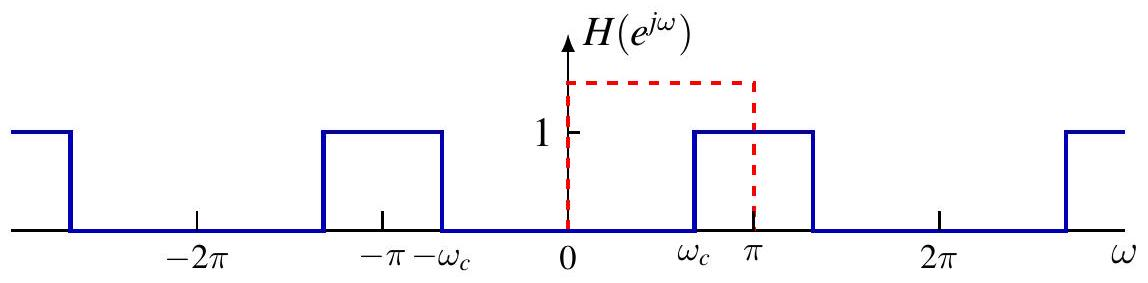
\includegraphics[keepaspectratio]{imglink/f0d10ac8-9b51-40af-8373-7a211a98e620-16.png}}
\end{frame}

\begin{frame}{理想频率选择性滤波器}
\protect\phantomsection\label{ux7406ux60f3ux9891ux7387ux9009ux62e9ux6027ux6ee4ux6ce2ux5668-3}
理想带通滤波器

\[
H\left(e^{j \omega}\right)= \begin{cases}1, & \omega_{c 1} \leq|\omega| \leq \omega_{c 2} \\ 0, & |\omega|<\omega_{c 1} \text { or } \omega_{c 2}<|\omega| \leq \pi\end{cases}
\]

\(\omega_{c 1}\) : 下截止频率， \(\omega_{c 2}\) : 上截止频率

\pandocbounded{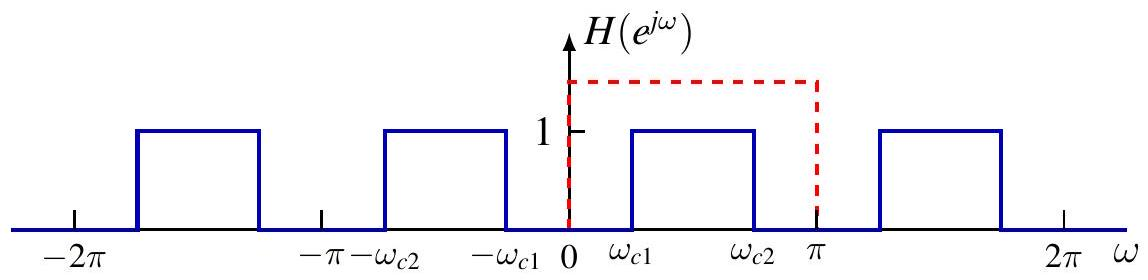
\includegraphics[keepaspectratio]{imglink/f0d10ac8-9b51-40af-8373-7a211a98e620-17.png}}
\end{frame}

\begin{frame}{一阶递归离散时间滤波器}
\protect\phantomsection\label{ux4e00ux9636ux9012ux5f52ux79bbux6563ux65f6ux95f4ux6ee4ux6ce2ux5668}
\[
y[n]-a y[n-1]=x[n]
\]

对于输入信号 \(x[n]=e^{j \omega n}\)，系统的输出为
\(y[n]=H\left(e^{j \omega}\right) e^{j \omega n}\)。

当 \(|a|<1\) 时，\textbf{频率响应}（Frequency response）有明确定义：

\[
H\left(e^{j \omega}\right)=\frac{1}{1-a e^{-j \omega}}, \quad|a|<1
\]

若将系数 \(a\) 表示为极坐标形式 \(a=|a| e^{j \phi}\)，则：

\textbf{幅度响应 (Magnitude Response):} \[
\left|H\left(e^{j \omega}\right)\right|=\frac{1}{\sqrt{1+|a|^{2}-2|a| \cos (\omega-\phi)}}
\]

\textbf{相位响应 (Phase Response):} \[
\arg H\left(e^{j \omega}\right)=\arctan \frac{-|a| \sin (\omega-\phi)}{1-|a| \cos (\omega-\phi)}
\]
\end{frame}

\begin{frame}{一阶递归离散时间滤波器}
\protect\phantomsection\label{ux4e00ux9636ux9012ux5f52ux79bbux6563ux65f6ux95f4ux6ee4ux6ce2ux5668-1}
\begin{columns}[T]
\begin{column}{0.5\linewidth}
对于 \(a>0\), 低通滤波器 (指数平滑)
\pandocbounded{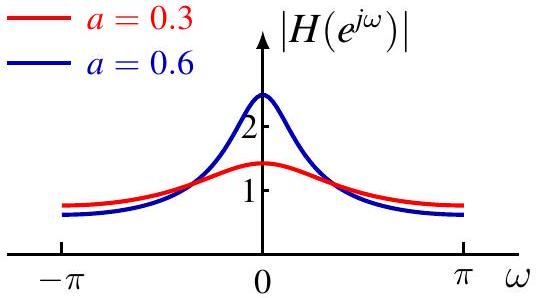
\includegraphics[keepaspectratio]{imglink/f0d10ac8-9b51-40af-8373-7a211a98e620-19.png}}

\pandocbounded{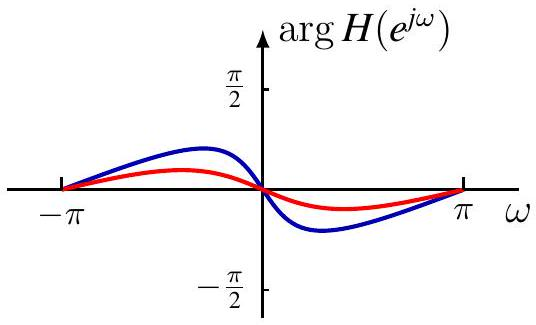
\includegraphics[keepaspectratio]{imglink/f0d10ac8-9b51-40af-8373-7a211a98e620-19_3.png}}
\end{column}

\begin{column}{0.5\linewidth}
对于 \(a<0\), 高通滤波器

\pandocbounded{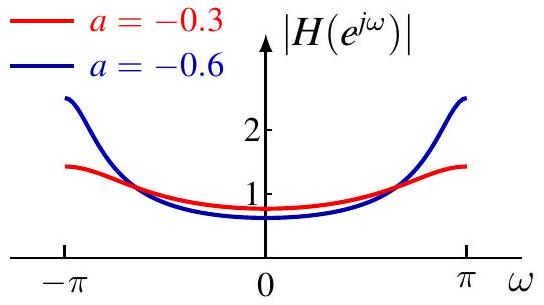
\includegraphics[keepaspectratio]{imglink/f0d10ac8-9b51-40af-8373-7a211a98e620-19_2.png}}

\pandocbounded{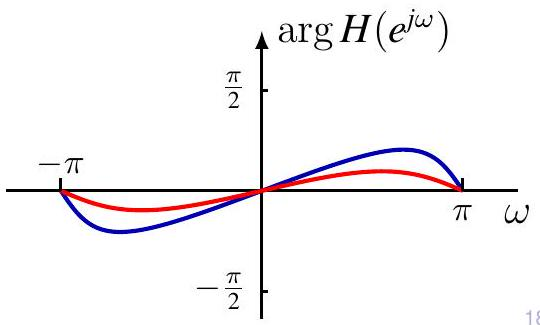
\includegraphics[keepaspectratio]{imglink/f0d10ac8-9b51-40af-8373-7a211a98e620-19_4.png}}
\end{column}
\end{columns}
\end{frame}

\begin{frame}{一阶递归离散时间滤波器}
\protect\phantomsection\label{ux4e00ux9636ux9012ux5f52ux79bbux6563ux65f6ux95f4ux6ee4ux6ce2ux5668-2}
\begin{columns}[T]
\begin{column}{0.5\linewidth}
\begin{block}{单位脉冲响应 (IIR 滤波器)}
\protect\phantomsection\label{ux5355ux4f4dux8109ux51b2ux54cdux5e94-iir-ux6ee4ux6ce2ux5668}
\[
\begin{gathered}
h[n]=a^{n} u[n] \\
H\left(e^{j \omega}\right)=\sum_{n=0}^{\infty}\left(a e^{-j \omega}\right)^{n}=\frac{1}{1-a e^{-j \omega}}
\end{gathered}
\]

为了保证级数\textbf{收敛}（Convergence），需要满足条件：\(|a|<1\)。
\end{block}

\begin{block}{阶跃响应 (Step Response)}
\protect\phantomsection\label{ux9636ux8dc3ux54cdux5e94-step-response}
\[
s[n]=(h * u)[n]=\frac{1-a^{n+1}}{1-a} u[n]
\]
\end{block}

\begin{block}{性能权衡 (Tradeoff)}
\protect\phantomsection\label{ux6027ux80fdux6743ux8861-tradeoff}
\begin{itemize}
\tightlist
\item
  \textbf{\(|a|\)
  较大时}：通带越窄（选择性更好），但响应速度越慢（时域拖尾更长）。
\item
  \textbf{\(|a|\) 较小时}：响应速度越快，但通带越宽（滤波效果较弱）。
\end{itemize}
\end{block}
\end{column}

\begin{column}{0.5\linewidth}
\pandocbounded{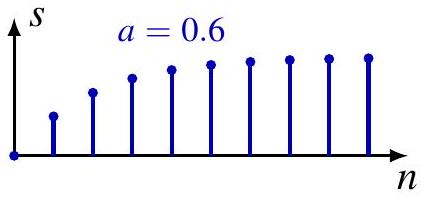
\includegraphics[keepaspectratio]{imglink/f0d10ac8-9b51-40af-8373-7a211a98e620-20_2.png}}

\pandocbounded{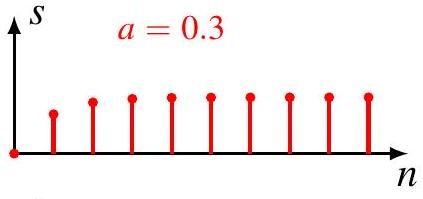
\includegraphics[keepaspectratio]{imglink/f0d10ac8-9b51-40af-8373-7a211a98e620-20_3.png}}

\pandocbounded{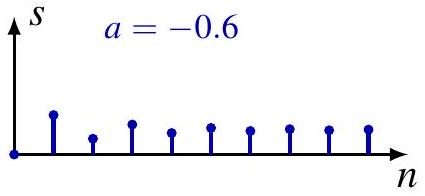
\includegraphics[keepaspectratio]{imglink/f0d10ac8-9b51-40af-8373-7a211a98e620-20.png}}

\pandocbounded{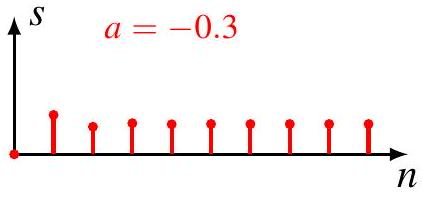
\includegraphics[keepaspectratio]{imglink/f0d10ac8-9b51-40af-8373-7a211a98e620-20_4.png}}
\end{column}
\end{columns}
\end{frame}

\begin{frame}{滑动平均作为低通滤波器}
\protect\phantomsection\label{ux6ed1ux52a8ux5e73ux5747ux4f5cux4e3aux4f4eux901aux6ee4ux6ce2ux5668}
\[
y[n]=\frac{1}{M_{1}+M_{2}+1} \sum_{k=-M_{1}}^{M_{2}} x[n-k]
\]

脉冲响应 (FIR 滤波器)

\[
h[n]=\frac{1}{M_{1}+M_{2}+1} \sum_{k=-M_{1}}^{M_{2}} \delta[n-k]
\]

频率响应

\[
H\left(e^{j \omega}\right)=\frac{1}{M_{1}+M_{2}+1} \sum_{k=-M_{1}}^{M_{2}} e^{-j k \omega}=\frac{e^{j \frac{M_{1}-M_{2}}{2} \omega}}{M_{1}+M_{2}+1} \frac{\sin \left(\frac{M_{1}+M_{2}+1}{2} \omega\right)}{\sin \frac{\omega}{2}}
\]
\end{frame}

\begin{frame}{滑动平均作为低通滤波器}
\protect\phantomsection\label{ux6ed1ux52a8ux5e73ux5747ux4f5cux4e3aux4f4eux901aux6ee4ux6ce2ux5668-1}
\(M_{1}=0, M_{2}=1\),

\[
\begin{aligned}
y[n] & =\frac{1}{2}(x[n]+x[n-1]) \\
h[n] & =\frac{1}{2}(\delta[n]+\delta[n-1]) \\
H\left(e^{j \omega}\right) & =e^{-j \frac{\omega}{2}} \cos \frac{\omega}{2}
\end{aligned}
\]

\pandocbounded{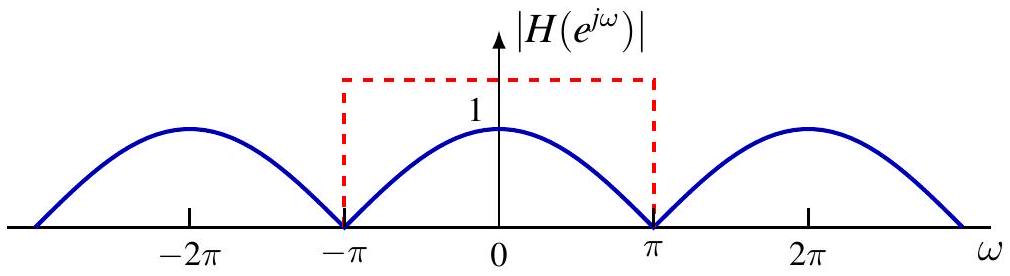
\includegraphics[keepaspectratio]{imglink/f0d10ac8-9b51-40af-8373-7a211a98e620-22.png}}

验证以下结论：

\begin{itemize}
\tightlist
\item
  若输入 \(x[n]=K e^{j 0 \cdot n}\)，则输出 \(y[n]=x[n]\)。
\item
  若输入 \(x[n]=K e^{j \pi n}=K(-1)^{n}\)，则输出 \(y[n]=0\)。
\end{itemize}
\end{frame}

\begin{frame}{滑动平均作为低通滤波器}
\protect\phantomsection\label{ux6ed1ux52a8ux5e73ux5747ux4f5cux4e3aux4f4eux901aux6ee4ux6ce2ux5668-2}
\(M_{1}=M_{2}=1\),

\[
\begin{aligned}
y[n] & =\frac{1}{3}(x[n+1]+x[n]+x[n-1]) \\
h[n] & =\frac{1}{3}(\delta[n+1]+\delta[n]+\delta[n-1]) \\
H\left(e^{j \omega}\right) & =\frac{\sin \left(\frac{3}{2} \omega\right)}{3 \sin \frac{\omega}{2}}=\frac{1}{3}+\frac{2}{3} \cos \omega
\end{aligned}
\]

\pandocbounded{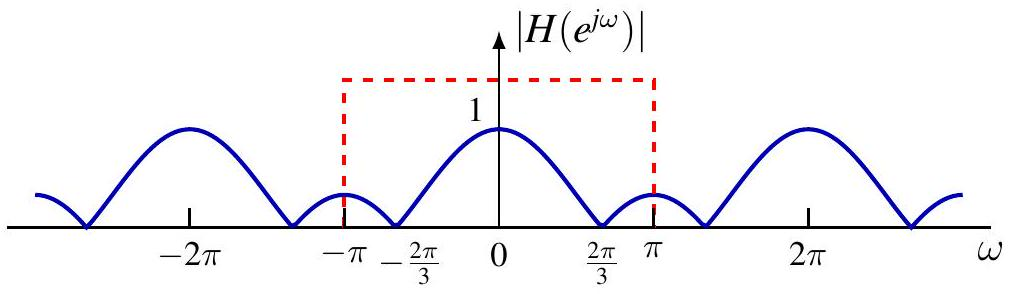
\includegraphics[keepaspectratio]{imglink/f0d10ac8-9b51-40af-8373-7a211a98e620-23.png}}
\end{frame}

\begin{frame}{滑动平均作为低通滤波器}
\protect\phantomsection\label{ux6ed1ux52a8ux5e73ux5747ux4f5cux4e3aux4f4eux901aux6ee4ux6ce2ux5668-3}
\[
H\left(e^{j \omega}\right)=\frac{e^{j \frac{M_{1}-M_{2}}{2} \omega}}{M_{1}+M_{2}+1} \frac{\sin \left(\frac{M_{1}+M_{2}+1}{2} \omega\right)}{\sin \frac{\omega}{2}}
\]

\[
M_{1}+M_{2}+1=11
\]

\begin{columns}[T]
\begin{column}{0.3\linewidth}
\end{column}

\begin{column}{0.4\linewidth}
\pandocbounded{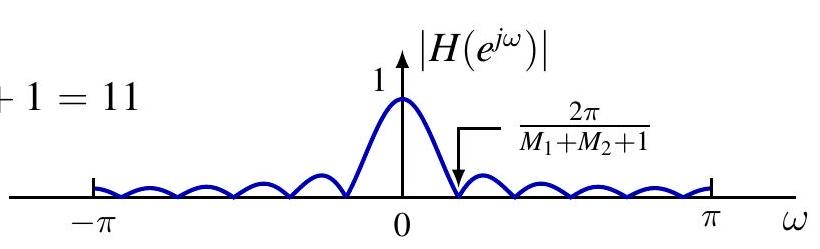
\includegraphics[keepaspectratio]{imglink/f0d10ac8-9b51-40af-8373-7a211a98e620-24_2.png}}
\end{column}

\begin{column}{0.3\linewidth}
\end{column}
\end{columns}

\[
M_{1}+M_{2}+1=41
\]

\begin{center}
\pandocbounded{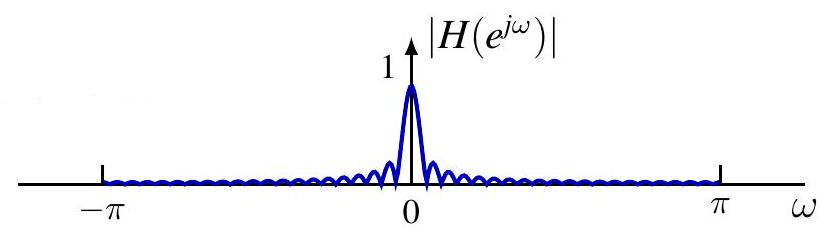
\includegraphics[keepaspectratio]{imglink/f0d10ac8-9b51-40af-8373-7a211a98e620-24.png}}
\end{center}

\(M_1 + M_2\) 越大，通带越窄，输出越平滑。
\end{frame}

\begin{frame}{滑动平均作为低通滤波器}
\protect\phantomsection\label{ux6ed1ux52a8ux5e73ux5747ux4f5cux4e3aux4f4eux901aux6ee4ux6ce2ux5668-4}
\begin{center}
\pandocbounded{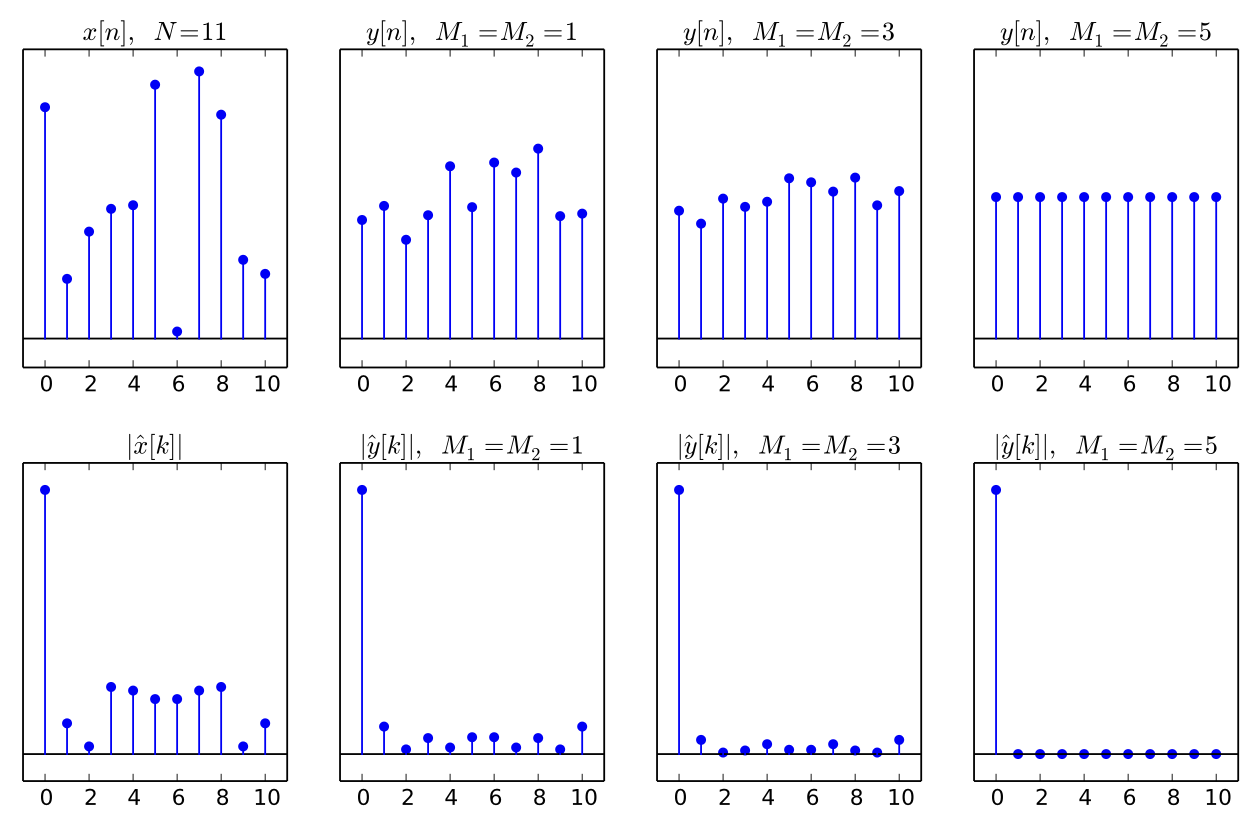
\includegraphics[keepaspectratio]{imglink/movingaveragelowfilter.png}}
\end{center}
\end{frame}

\begin{frame}{滑动平均作为低通滤波器}
\protect\phantomsection\label{ux6ed1ux52a8ux5e73ux5747ux4f5cux4e3aux4f4eux901aux6ee4ux6ce2ux5668-5}
\begin{block}{非因果系统 (Noncausal)}
\protect\phantomsection\label{ux975eux56e0ux679cux7cfbux7edf-noncausal}
\[
y_{1}[n]=\frac{1}{2 M+1} \sum_{k=-M}^{M} x[n-k]
\]
\end{block}

\begin{block}{因果系统 (Causal)}
\protect\phantomsection\label{ux56e0ux679cux7cfbux7edf-causal}
\[
y_{2}[n]=\frac{1}{2 M+1} \sum_{k=0}^{2 M} x[n-k]
\]

注：\(y_{2}=\tau_{M} y_{1}\)（即 \(y_2\) 是 \(y_1\) 延迟了 \(M\)
个样本的结果）。
\end{block}

\begin{block}{对于实时系统 (Real-time system)}
\protect\phantomsection\label{ux5bf9ux4e8eux5b9eux65f6ux7cfbux7edf-real-time-system}
\begin{itemize}
\tightlist
\item
  \textbf{非因果版本不可实现}：因为它需要利用``未来''的样本点。
\item
  \textbf{因果版本可实现}：仅利用当前及过去的样本点。
\item
  \textbf{性能权衡}：\(M\)
  越大，通带越窄，输出越平滑，但\textbf{延迟越长}，响应越\textbf{迟缓}。
\end{itemize}
\end{block}
\end{frame}

\begin{frame}{一阶差分作为高通滤波器}
\protect\phantomsection\label{ux4e00ux9636ux5deeux5206ux4f5cux4e3aux9ad8ux901aux6ee4ux6ce2ux5668}
缩放一阶差分（平减一阶差分）

\[
y[n]=\frac{1}{2}(x[n]-x[n-1])
\]

脉冲响应 (FIR滤波器)

\[
h[n]=\frac{1}{2}(\delta[n]-\delta[n-1])
\]

\begin{columns}[T]
\begin{column}{0.5\linewidth}
\begin{block}{频率响应 (Frequency Response)}
\protect\phantomsection\label{ux9891ux7387ux54cdux5e94-frequency-response}
\[
\begin{aligned}
H\left(e^{j \omega}\right) & =\frac{1}{2}\left(1-e^{-j \omega}\right)=j e^{-j \frac{\omega}{2}} \sin \frac{\omega}{2} \\
\left|H\left(e^{j \omega}\right)\right| & =\left|\sin \frac{\omega}{2}\right|
\end{aligned}
\]
\end{block}

\begin{block}{结论验证 (Verification)}
\protect\phantomsection\label{ux7ed3ux8bbaux9a8cux8bc1-verification}
\begin{itemize}
\tightlist
\item
  若输入 \(x[n]=K e^{j 0 \cdot n}\)（直流分量），则输出 \(y[n]=0\)。
\item
  若输入 \(x[n]=K e^{j \pi n}=K(-1)^{n}\)（最高频分量），则输出
  \(y[n]=x[n]\)。
\end{itemize}
\end{block}
\end{column}

\begin{column}{0.5\linewidth}
\pandocbounded{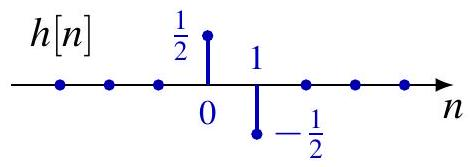
\includegraphics[keepaspectratio]{imglink/f0d10ac8-9b51-40af-8373-7a211a98e620-27.png}}

\pandocbounded{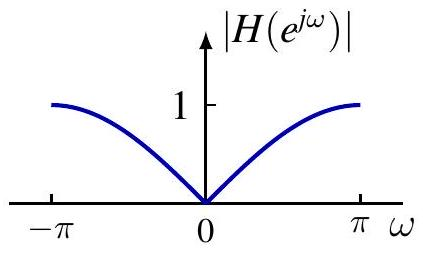
\includegraphics[keepaspectratio]{imglink/f0d10ac8-9b51-40af-8373-7a211a98e620-27_2.png}}
\end{column}
\end{columns}
\end{frame}

\begin{frame}{一阶差分用于边缘检测}
\protect\phantomsection\label{ux4e00ux9636ux5deeux5206ux7528ux4e8eux8fb9ux7f18ux68c0ux6d4b}
\begin{center}
\pandocbounded{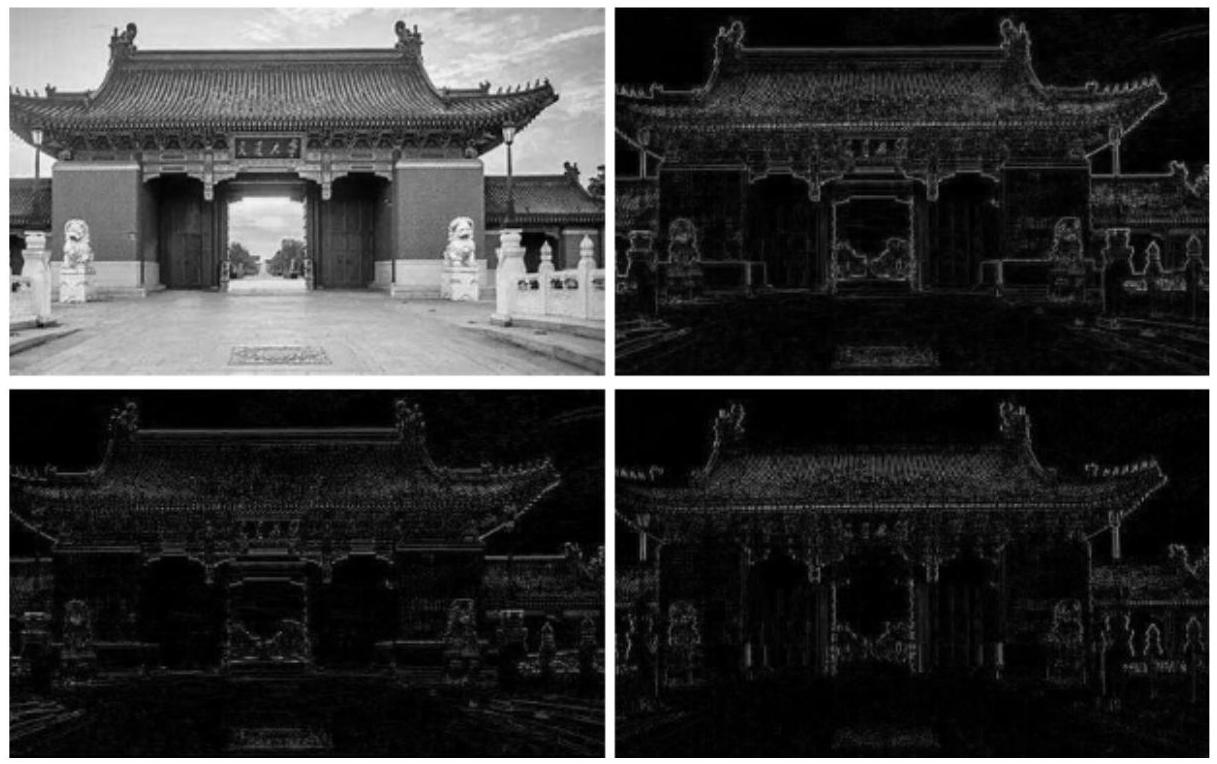
\includegraphics[keepaspectratio]{imglink/f0d10ac8-9b51-40af-8373-7a211a98e620-28.png}}
\end{center}
\end{frame}

\begin{frame}{作业}
\protect\phantomsection\label{ux4f5cux4e1a}
\end{frame}

\begin{frame}
第三章 周期信号的傅里叶级数表示 完
\end{frame}




\end{document}
